% Options for packages loaded elsewhere
% Options for packages loaded elsewhere
\PassOptionsToPackage{unicode}{hyperref}
\PassOptionsToPackage{hyphens}{url}
\PassOptionsToPackage{dvipsnames,svgnames,x11names}{xcolor}
%
\documentclass[
  11pt,
]{book}
\usepackage{xcolor}
\usepackage{amsmath,amssymb}
\setcounter{secnumdepth}{5}
\usepackage{iftex}
\ifPDFTeX
  \usepackage[T1]{fontenc}
  \usepackage[utf8]{inputenc}
  \usepackage{textcomp} % provide euro and other symbols
\else % if luatex or xetex
  \usepackage{unicode-math} % this also loads fontspec
  \defaultfontfeatures{Scale=MatchLowercase}
  \defaultfontfeatures[\rmfamily]{Ligatures=TeX,Scale=1}
\fi
\usepackage{lmodern}
\ifPDFTeX\else
  % xetex/luatex font selection
\fi
% Use upquote if available, for straight quotes in verbatim environments
\IfFileExists{upquote.sty}{\usepackage{upquote}}{}
\IfFileExists{microtype.sty}{% use microtype if available
  \usepackage[]{microtype}
  \UseMicrotypeSet[protrusion]{basicmath} % disable protrusion for tt fonts
}{}
\makeatletter
\@ifundefined{KOMAClassName}{% if non-KOMA class
  \IfFileExists{parskip.sty}{%
    \usepackage{parskip}
  }{% else
    \setlength{\parindent}{0pt}
    \setlength{\parskip}{6pt plus 2pt minus 1pt}}
}{% if KOMA class
  \KOMAoptions{parskip=half}}
\makeatother
% Make \paragraph and \subparagraph free-standing
\makeatletter
\ifx\paragraph\undefined\else
  \let\oldparagraph\paragraph
  \renewcommand{\paragraph}{
    \@ifstar
      \xxxParagraphStar
      \xxxParagraphNoStar
  }
  \newcommand{\xxxParagraphStar}[1]{\oldparagraph*{#1}\mbox{}}
  \newcommand{\xxxParagraphNoStar}[1]{\oldparagraph{#1}\mbox{}}
\fi
\ifx\subparagraph\undefined\else
  \let\oldsubparagraph\subparagraph
  \renewcommand{\subparagraph}{
    \@ifstar
      \xxxSubParagraphStar
      \xxxSubParagraphNoStar
  }
  \newcommand{\xxxSubParagraphStar}[1]{\oldsubparagraph*{#1}\mbox{}}
  \newcommand{\xxxSubParagraphNoStar}[1]{\oldsubparagraph{#1}\mbox{}}
\fi
\makeatother


\usepackage{longtable,booktabs,array}
\usepackage{calc} % for calculating minipage widths
% Correct order of tables after \paragraph or \subparagraph
\usepackage{etoolbox}
\makeatletter
\patchcmd\longtable{\par}{\if@noskipsec\mbox{}\fi\par}{}{}
\makeatother
% Allow footnotes in longtable head/foot
\IfFileExists{footnotehyper.sty}{\usepackage{footnotehyper}}{\usepackage{footnote}}
\makesavenoteenv{longtable}
\usepackage{graphicx}
\makeatletter
\newsavebox\pandoc@box
\newcommand*\pandocbounded[1]{% scales image to fit in text height/width
  \sbox\pandoc@box{#1}%
  \Gscale@div\@tempa{\textheight}{\dimexpr\ht\pandoc@box+\dp\pandoc@box\relax}%
  \Gscale@div\@tempb{\linewidth}{\wd\pandoc@box}%
  \ifdim\@tempb\p@<\@tempa\p@\let\@tempa\@tempb\fi% select the smaller of both
  \ifdim\@tempa\p@<\p@\scalebox{\@tempa}{\usebox\pandoc@box}%
  \else\usebox{\pandoc@box}%
  \fi%
}
% Set default figure placement to htbp
\def\fps@figure{htbp}
\makeatother


% definitions for citeproc citations
\NewDocumentCommand\citeproctext{}{}
\NewDocumentCommand\citeproc{mm}{%
  \begingroup\def\citeproctext{#2}\cite{#1}\endgroup}
\makeatletter
 % allow citations to break across lines
 \let\@cite@ofmt\@firstofone
 % avoid brackets around text for \cite:
 \def\@biblabel#1{}
 \def\@cite#1#2{{#1\if@tempswa , #2\fi}}
\makeatother
\newlength{\cslhangindent}
\setlength{\cslhangindent}{1.5em}
\newlength{\csllabelwidth}
\setlength{\csllabelwidth}{3em}
\newenvironment{CSLReferences}[2] % #1 hanging-indent, #2 entry-spacing
 {\begin{list}{}{%
  \setlength{\itemindent}{0pt}
  \setlength{\leftmargin}{0pt}
  \setlength{\parsep}{0pt}
  % turn on hanging indent if param 1 is 1
  \ifodd #1
   \setlength{\leftmargin}{\cslhangindent}
   \setlength{\itemindent}{-1\cslhangindent}
  \fi
  % set entry spacing
  \setlength{\itemsep}{#2\baselineskip}}}
 {\end{list}}
\usepackage{calc}
\newcommand{\CSLBlock}[1]{\hfill\break\parbox[t]{\linewidth}{\strut\ignorespaces#1\strut}}
\newcommand{\CSLLeftMargin}[1]{\parbox[t]{\csllabelwidth}{\strut#1\strut}}
\newcommand{\CSLRightInline}[1]{\parbox[t]{\linewidth - \csllabelwidth}{\strut#1\strut}}
\newcommand{\CSLIndent}[1]{\hspace{\cslhangindent}#1}



\setlength{\emergencystretch}{3em} % prevent overfull lines

\providecommand{\tightlist}{%
  \setlength{\itemsep}{0pt}\setlength{\parskip}{0pt}}



 


% --- Customised preamble.tex begins here ---
\usepackage[a4paper]{geometry}
\usepackage[british]{babel}
\frenchspacing
\tolerance=400
\emergencystretch=3em
\hyphenpenalty=20

\usepackage{microtype}
\microtypesetup{
  tracking   = true,
  protrusion = true,
  expansion  = true,
  factor     = 1100,
  stretch    = 15,
  shrink     = 15,
}

\let\oldtexttt\texttt
\renewcommand{\texttt}[1]{\oldtexttt{\small #1}}
\usepackage{etoolbox}
\AtBeginEnvironment{Highlighting}{\footnotesize}
\AtBeginEnvironment{verbatim}{\footnotesize}
\AtBeginEnvironment{Shaded}{\footnotesize}

% ——————————————————————————————————————————————
% Fontspec and typography
% ——————————————————————————————————————————————
\usepackage{fontspec}
\usepackage{amsmath}
\usepackage{luatexja}

% Serif body text → TeX Gyre Pagella (Palatino)
% \setmainfont[
%   UprightFont    = *-Regular,
%   ItalicFont     = *-Italic,
%   BoldFont       = *-Bold,
%   BoldItalicFont = *-BoldItalic,
%   Ligatures      = TeX,
%   Numbers        = {OldStyle, Proportional}
% ]{TeX Gyre Pagella}

\usepackage{unicode-math}
\setmainfont{STIX Two Text}
\setmathfont{STIX Two Math}
\usepackage{mhchem}  % Chemical formula support

% Sans‐serif headings → Fira Sans (with TeX discretionary ligatures)
\setsansfont[
  UprightFont    = *-Regular,
  ItalicFont     = *-Italic,
  BoldFont       = *-Bold,
  BoldItalicFont = *-BoldItalic,
  Ligatures      = {TeX, Common, Discretionary},
  Numbers        = {Proportional}
]{Fira Sans}

% Monospace Font
\setmonofont[Scale=0.89]{FiraCode Nerd Font}

% Math Font (compatible with Pagella)
% \setmathfont{TeX Gyre Pagella Math}

% Configure all section titles to use the sans font
\usepackage{sectsty}
\allsectionsfont{\sffamily}

% Logo and title customization
\usepackage{graphicx}
\usepackage{titling}

% Disable default title hooks
\pretitle{}
\posttitle{}

% Disable Pandoc’s own title machinery
\renewcommand{\title}[1]{}
\renewcommand{\author}[1]{}
\renewcommand{\date}[1]{}

% Custom title page layout
\renewcommand{\maketitle}{%
  \begin{titlepage}
    \centering
    % Logos at top
    
\includegraphics[height=3cm]{../Faculty_logo.png}\hspace{2cm}
    
\includegraphics[height=3cm]{../UWC_logo.png}\\[2em]

    % Title lines in large bold
    {\huge\bfseries
      BCB334 Biogeography \& Global Ecology Lecture Series, July 2025\\[0.5em]
      Biodiversity \& Conservation Biology Department\\[0.5em]
      University of the Western Cape\\[3em]
    }

    % Center vertically the descriptive paragraph
    \vfill
    {\large
      Author: Professor AJ Smit.\\[1em]
      This document contains transcripts from my online lectures prepared during the COVID-19 years of 2020 and 2021.\par
    }
    \vfill
  \end{titlepage}
}

% Auto-invoke title and ToC at start
\AtBeginDocument{%
  \maketitle
  \tableofcontents
  \newpage
}
\makeatletter
\@ifpackageloaded{tcolorbox}{}{\usepackage[skins,breakable]{tcolorbox}}
\@ifpackageloaded{fontawesome5}{}{\usepackage{fontawesome5}}
\definecolor{quarto-callout-color}{HTML}{909090}
\definecolor{quarto-callout-note-color}{HTML}{0758E5}
\definecolor{quarto-callout-important-color}{HTML}{CC1914}
\definecolor{quarto-callout-warning-color}{HTML}{EB9113}
\definecolor{quarto-callout-tip-color}{HTML}{00A047}
\definecolor{quarto-callout-caution-color}{HTML}{FC5300}
\definecolor{quarto-callout-color-frame}{HTML}{acacac}
\definecolor{quarto-callout-note-color-frame}{HTML}{4582ec}
\definecolor{quarto-callout-important-color-frame}{HTML}{d9534f}
\definecolor{quarto-callout-warning-color-frame}{HTML}{f0ad4e}
\definecolor{quarto-callout-tip-color-frame}{HTML}{02b875}
\definecolor{quarto-callout-caution-color-frame}{HTML}{fd7e14}
\makeatother
\makeatletter
\@ifpackageloaded{caption}{}{\usepackage{caption}}
\AtBeginDocument{%
\ifdefined\contentsname
  \renewcommand*\contentsname{Table of contents}
\else
  \newcommand\contentsname{Table of contents}
\fi
\ifdefined\listfigurename
  \renewcommand*\listfigurename{List of Figures}
\else
  \newcommand\listfigurename{List of Figures}
\fi
\ifdefined\listtablename
  \renewcommand*\listtablename{List of Tables}
\else
  \newcommand\listtablename{List of Tables}
\fi
\ifdefined\figurename
  \renewcommand*\figurename{Figure}
\else
  \newcommand\figurename{Figure}
\fi
\ifdefined\tablename
  \renewcommand*\tablename{Table}
\else
  \newcommand\tablename{Table}
\fi
}
\@ifpackageloaded{float}{}{\usepackage{float}}
\floatstyle{ruled}
\@ifundefined{c@chapter}{\newfloat{codelisting}{h}{lop}}{\newfloat{codelisting}{h}{lop}[chapter]}
\floatname{codelisting}{Listing}
\newcommand*\listoflistings{\listof{codelisting}{List of Listings}}
\makeatother
\makeatletter
\makeatother
\makeatletter
\@ifpackageloaded{caption}{}{\usepackage{caption}}
\@ifpackageloaded{subcaption}{}{\usepackage{subcaption}}
\makeatother
\usepackage{bookmark}
\IfFileExists{xurl.sty}{\usepackage{xurl}}{} % add URL line breaks if available
\urlstyle{same}
\hypersetup{
  pdfauthor={Smit, A. J.},
  colorlinks=true,
  linkcolor={purple},
  filecolor={blue},
  citecolor={blue},
  urlcolor={blue},
  pdfcreator={LaTeX via pandoc}}


\author{Smit, A. J.}
\date{}
\begin{document}
\frontmatter


\mainmatter
\makeatletter
\renewcommand{\chaptername}{Lecture}
\renewcommand{\@chapapp}{Lecture}
\makeatother


\includegraphics[width=\linewidth,height=3cm,keepaspectratio]{../Faculty_logo.png}

\includegraphics[width=\linewidth,height=4cm,keepaspectratio]{../UWC_logo.png}

\chapter*{Preface}\label{preface}
\addcontentsline{toc}{chapter}{Preface}

This book contains the transcripts from the BDC334 lectures that I gave
during the COVID-19 year of 2020. The lectures were recorded and made
available to students online, and the transcripts were created to
accompany those video recordings. The content of these lectures is still
relevant today (in fact, the content has not changed much), and I hope
that they will be useful for students studying macroecology.

The transcripts were created using the
\href{https://superwhisper.com}{SuperWhisper} AI tool, which uses a
combination of machine learning and natural language processing
techniques (GPT-4.1 + the Ulta voice model) to transcribe the audio
recordings into text. The transcripts were then edited for clarity and
accuracy. The prompt I used to convert the audio is:

\begin{verbatim}
GENERAL:
- Use British English consistently and religiously.
- Please transcribe the video or sound file, keeping more or
  less my mode and style of speaking intact. 
- The intention is to maintain a style of writing that
  closely mirrors my natural way of speaking.
- Apply corrections to ensure my grammar and language are
  clear and correct after translation to text. 
- Use proper paragraphs, and apply punctuation liberally.
- Apply strict fact-checking. Indicate, where necessary,
  where the factual material that I talk about is clearly
  incorrect. Insert a pointer such as 'attention' in square
  brackets next to the statement that has some doubt
  associated with it.
- The audience is the undergraduate university class who sits
  in my lectures. 
- The intended use of the material will be to serve as a
  faithful reproduction of my lecture content as presented in
  the voice or video material that I supply.
- Translate any numbers with units or math to LaTeX math and
  wrap the command in $ … $ for use in Quarto. E.g.,
  2,500–3,000 μmol m⁻² s⁻¹ becomes
  $\(2{,}500\text{--}3{,}000\;\mu\mathrm{mol}\,
  \mathrm{m}^{-2}\, \mathrm{s}^{-1}\)$.

NOTES ON FORMATTING:
- Please start with the highest-level heading (#) that has
  the name of the transcribed file, such as “# Lecture
  Transcript: Plant Stresses”, ommitting any reference to the
  module name or lecture number.
- Insert deeper level headings (## and ###) as necessary to
  add some structure to the textual content. 
- If you are able to reference the transcribed text to a
  slide number, please do so.
 
IMPORTANT:
- Don’t add any embellishments, such as acknowledging my
  request or conclusion statement. Simply return the
  transcribed text.
\end{verbatim}

\chapter{Background and Expectations}\label{background-and-expectations}

\chapter*{Lecture 1}\label{lecture-1}
\addcontentsline{toc}{chapter}{Lecture 1}

\section{The Core Material}\label{the-core-material}

Please consider the lecture transcripts in this book as the core
material for your BDC334 course --- an online version of this same
material is provided on my Tangled Bank website, together with
additional web pages pertaining to BDC334. Have a look there for further
information. Those materials provide supplementary information and
should be read alongside the content contained within this book.
Everything there is examinable.

On the Tangled Bank, you will also find links to the various practical
sessions (the Labs). In addition, some data necessary for completing the
various laboratory exercises can be downloaded from there. A range of
other information is available as well.

On the ``About'' page, on the left-hand side under the BDC334 website
link on Tangled Bank, you will find details about the lecture schedule,
when the practical sessions occur, and a collection of other necessary
information you will need throughout this module. I will also list the
dates and times of the two class tests that you are expected to complete
during the course of this module.

\section{The Importance of Reading in Scientific
Training}\label{the-importance-of-reading-in-scientific-training}

A point I want to emphasise --- perhaps at the risk of sounding
old-fashioned --- is the necessity of reading detailed, long-form
scientific literature. Many students, nowadays, prefer consuming
information in bite-sized chunks that fit onto a mobile phone screen;
however, scientific knowledge and argumentation require sustained
engagement with complete texts. This is the mode of teaching that
informed my own education 20 or 30 years ago, and it remains
indispensable for your intellectual development. The technical expertise
in this module is largely around matrix interpretation, not computation;
your focus should be on synthesising qualitative knowledge across
sources.

Your assessments will involve long-form, essay-type questions, not
superficial answers drawn from isolated papers. You will be expected to
draw upon and integrate your understanding from several readings with
the lecture material into a cohesive response. This kind of applied
knowledge is necessary, not just for in-person or remote assessments,
but also in professional scientific communication.

Therefore, online, alongside the lecture material and accompanying
slides, I'll be providing various papers for you to read. Direct links
to the papers are provided --- follow those links to download them. I
expect you to read and understand all these papers. If there's anything
you don't grasp, please discuss it with your classmates or arrange an
appointment with me --- either in a group of three, four, or more --- on
Monday afternoons, Wednesday mornings, or Thursday afternoons during the
practical sessions. You can schedule meetings with me then to discuss
such matters.

The following papers are \emph{expected} to be read as part of many of
the upcoming lectures. Please keep an eye out in the lectures for
specific mention of these papers and make sure that you read them well
in advance of attending my lectures. Everything in these papers is
examinable and you are expected to read all of it and know all of it.
The expected additional reading includes the following (their full
titles are in the References section at the end):

Week 1:

\begin{itemize}
\tightlist
\item
  Keith et al. (2012)
\item
  Shade et al. (2018)
\item
  McGill (2019)
\end{itemize}

Week 2:

\begin{itemize}
\tightlist
\item
  Nekola and White (1999)
\item
  Smit et al. (2017)
\item
  Tittensor et al. (2010)
\end{itemize}

Week 3:

\begin{itemize}
\tightlist
\item
  Shade et al. (2018)
\end{itemize}

Week 4:

\begin{itemize}
\tightlist
\item
  Chapin III et al. (2000)
\item
  Gotelli and Chao (2013)
\item
  Maxwell et al. (2016)
\item
  Tilman et al. (2017)
\end{itemize}

Week 5:

\begin{itemize}
\tightlist
\item
  Burger et al. (2012)
\item
  Costanza et al. (1997)
\item
  Costanza et al. (2014)
\end{itemize}

There are also several other papers that I mention throughout all the
lectures. These are intended to provide background information that will
assist you in understanding the lecture content a bit better. Unlike the
papers mentioned above, it is not expected that you read, know, and
fully understand them; however, they are important for providing
additional context that will facilitate your understanding of specific
issues raised in some of the labs and certain lectures.

\section{Developing Your Own Study Framework and Academic
Integrity}\label{developing-your-own-study-framework-and-academic-integrity}

If you feel, after reading these assigned papers, that your
comprehension is inadequate, take the initiative to seek further
information in the primary scientific literature. It is not sufficient
to rely solely on the specific documents I have distributed; critical
engagement with broader literature is a core expectation at university
level.

In terms of referencing, please note: websites are generally not
accepted as valid sources. Peer-reviewed publications, indicated in the
reference lists of your readings, are the standard. This is the academic
protocol you should follow---building up your knowledge from
scientifically credible sources.

Some of you have enquired about the need for textbooks. While textbooks
can be helpful, they are ultimately compilations of information
available in the primary literature. The expectation is that, as mature
university students, you will be able to navigate primary sources as
needed.

As always, if you have questions or are struggling with particular
concepts, you are welcome to reach out to me---on WhatsApp, by email, or
during Wednesday morning lectures.

\section{Labs}\label{labs}

During the course of this module, there will be four labs, or
practicals. These labs will take place on the fifth floor computer lab
of the Biodiversity and Conservation Biology Department building. It is
expected that you attend all of these practicals.

For those of you who have your own personal computers or laptops, please
bring them with you. It will probably help you a great deal if you get
the necessary software set up on your own computers. The demonstrator
and I will guide you through the installation processes and ensure that
you have the required software, R and RStudio, installed on your
laptops.

If you do not have a laptop, you are welcome to use the facilities in
the computer lab. All of the workstations there have the necessary
software installed.

During the first week, we will do some exercises in Excel. Thereafter,
in the following week, we will provide a brief introduction to the
software R, running within RStudio.

For those of you who are apprehensive about using scripting or coding
languages, please note it is a necessary component of modern ecological
research. So, the intention of these next few weeks is to give you a
brief, introductory background into scripting languages, with the aim of
solving some ecologically relevant problems.

Throughout all of these exercises, both myself and the demonstrator will
be available, walking around the floor to assist you with any questions
that you might have. Thank you.

\subsection{Lab 1}\label{lab-1}

This Lab accompanies the following lectures:

\begin{itemize}
\tightlist
\item
  Chapter~\ref{sec-lect5} on Multivariate Data and the rest of this
  page.
\end{itemize}

The data for this Lab pertains to the Doubs River (Verneaux 1973;
Borcard et al. 2011) study and some toy data, which may be found at the
links below:

\begin{itemize}
\tightlist
\item
  The environmental data --
  \href{../data/DoubsEnv.csv}{\texttt{DoubsEnv.csv}}
\item
  The species data -- \href{../data/DoubsSpe.csv}{\texttt{DoubsSpe.csv}}
\item
  The spatial data -- \href{../data/DoubsSpa.csv}{\texttt{DoubsSpa.csv}}
\item
  Example xyz data --
  \href{../data/Euclidean_distance_demo_data_xyz.csv}{\texttt{Euclidean\_distance\_demo\_data\_xyz.csv}}
\end{itemize}

\subsection{Lab 2}\label{lab-2}

Labs 2a and 2b accompany the following lecture:

\begin{itemize}
\tightlist
\item
  Chapter~\ref{sec-lect5} (in this book) on Multivariate Data and the
  rest of this page.
\end{itemize}

Lab 2b uses these data:

\begin{itemize}
\tightlist
\item
  Example xyz data --
  \href{../data/Euclidean_distance_demo_data_xyz.csv}{\texttt{Euclidean\_distance\_demo\_data\_xyz.csv}}
\item
  Example env data --
  \href{../data/Euclidean_distance_demo_data_env.csv}{\texttt{Euclidean\_distance\_demo\_data\_env.csv}}
\item
  The seaweed environmental data (Smit et al. 2017) --
  \href{../data/seaweed/SeaweedEnv.RData}{\texttt{SeaweedEnv.RData}}
\item
  The seaweed coastal sections (sites) --
  \href{../data/seaweed/SeaweedSites.csv}{\texttt{SeaweedSites.csv}}
\item
  The Doubs River environmental data --
  \href{../data/DoubsEnv.csv}{\texttt{DoubsEnv.csv}}
\end{itemize}

\subsection{Lab 3}\label{lab-3}

This Lab accompanies the following lecture:

\begin{itemize}
\tightlist
\item
  \href{Lec-04-biodiversity.html}{Lecture 4: Biodiversity Concepts}
\end{itemize}

The data for this Lab are the seaweed (Smit et al. 2017) as well as some
toy data at the links below:

\begin{itemize}
\tightlist
\item
  The seaweed species data --
  \href{../data/seaweed/SeaweedSpp.csv}{\texttt{SeaweedSpp.csv}}
\item
  The seaweed environmental data --
  \href{../data/seaweed/SeaweedEnv.csv}{\texttt{SeaweedEnv.csv}}
\item
  The seaweed coastal sections --
  \href{../data/seaweed/SeaweedSites.csv}{\texttt{SeaweedSites.csv}}
\item
  The fictitious light data
  \href{../data/light_levels.csv}{\texttt{light\_levels.csv}}
\end{itemize}

\subsection{Lab 4}\label{lab-4}

Finally, this Lab accompanies:

\begin{itemize}
\tightlist
\item
  \href{Lec-06-unified-ecology.html}{Lecture 6: Unified Ecology}
\end{itemize}

The data for this Lab include:

\begin{itemize}
\tightlist
\item
  The Barro Colorado Island Tree Counts data (Condit et al. 2002) --
  load \textbf{vegan} and load the data with \texttt{data(BCI)}
\item
  The Oribatid mite data (Borcard et al. 1992; Borcard and Legendre
  1994) -- load \textbf{vegan} and load the data with
  \texttt{data(mite)}
\item
  The seaweed species data (Smit et al. 2017) --
  \href{../data/seaweed/SeaweedSpp.csv}{\texttt{SeaweedSpp.csv}}
\item
  The Doubs River species data (Verneaux 1973; Borcard et al. 2011) --
  \href{../data/DoubsSpe.csv}{\texttt{DoubsSpe.csv}}
\end{itemize}

\section{Questions \& Answers}\label{questions-answers}

Before you approach me with questions about the coursework, I'd like you
to do one thing: explain your thought processes up to the point where
you get stuck. So, for example, if you have a question about some aspect
of, say for argument's sake, beta diversity, then before I answer your
question, I want you to explain what you've thought about beta diversity
thus far and where you become stuck --- where your thinking could not
proceed. Once you can demonstrate your reasoning process up until that
point, I'll be happy to take over from there. I do need some evidence
from you that you've honestly tried --- either individually or in
collaboration with others in the class --- to develop an explanation for
the area you're finding difficult.

Okay. Let's start with the lectures.

\chapter{Overview of Ecosystems}\label{overview-of-ecosystems}

\begin{tcolorbox}[enhanced jigsaw, colback=white, bottomrule=.15mm, opacitybacktitle=0.6, arc=.35mm, opacityback=0, left=2mm, coltitle=black, colframe=quarto-callout-note-color-frame, breakable, bottomtitle=1mm, toptitle=1mm, toprule=.15mm, titlerule=0mm, leftrule=.75mm, title=\textcolor{quarto-callout-note-color}{\faInfo}\hspace{0.5em}{BCB743}, colbacktitle=quarto-callout-note-color!10!white, rightrule=.15mm]

This material must be reviewed by BCB743 students in Week 1 of
Quantitative Ecology.

\end{tcolorbox}

\chapter*{Lecture 2a}\label{lecture-2a}
\addcontentsline{toc}{chapter}{Lecture 2a}

\section{Papers to Read}\label{papers-to-read}

The first very important paper that you need to read discusses the whole
concept of macroecology. The paper was written by Sally Keith and her
colleagues, and it was published in \(2012\). What is macroecology? It
deals with the development of the field over the past \(30\text{--}35\)
years or so, since the coining of the term by Brown and Maurer (1989).
The paper highlights the necessity of understanding the processes that
are linked to the development of structure in biodiversity across the
face of Earth. Additionally, it addresses the breaking down of barriers
that existed between ``old-fashioned'' population and community ecology,
moving instead towards a far more comprehensive and integrated view of
ecology. This integrated perspective brings together knowledge acquired
from a wide variety of new applications.

Please read that paper, as it is quite foundational to the development
of your understanding of the concept of macroecology.

The second foundational paper for this week is by Ashley Shade and
colleagues published in 2018. It is going to emerge several times during
the course of this module, such as in Lecture 3 and Lecture 5. This is
essentially a review detailing the core principles of macroecology. It
aims to unite ecological understanding across various scales, ranging
from the very small to the very large, and spanning local spatial
interactions through to global patterns.

Particularly notable within this paper are what can almost be called
`laws' of biodiversity. These are general patterns and principles that
recur consistently, whether in microbes like bacteria and archaea, or in
much larger organisms such as blue whales. The population dynamics that
apply to small organisms also scale to larger ones, reinforcing the
universality of certain ecological dynamics.

However, you must not study the material from this paper in isolation
from its broader context. The definitions and key ideas---some of which
I have highlighted for you---are crucial, but they must be considered
within the flow of the entire document.

\section{Introduction to Ecosystems}\label{introduction-to-ecosystems}

\begin{figure}[ht]
\centering
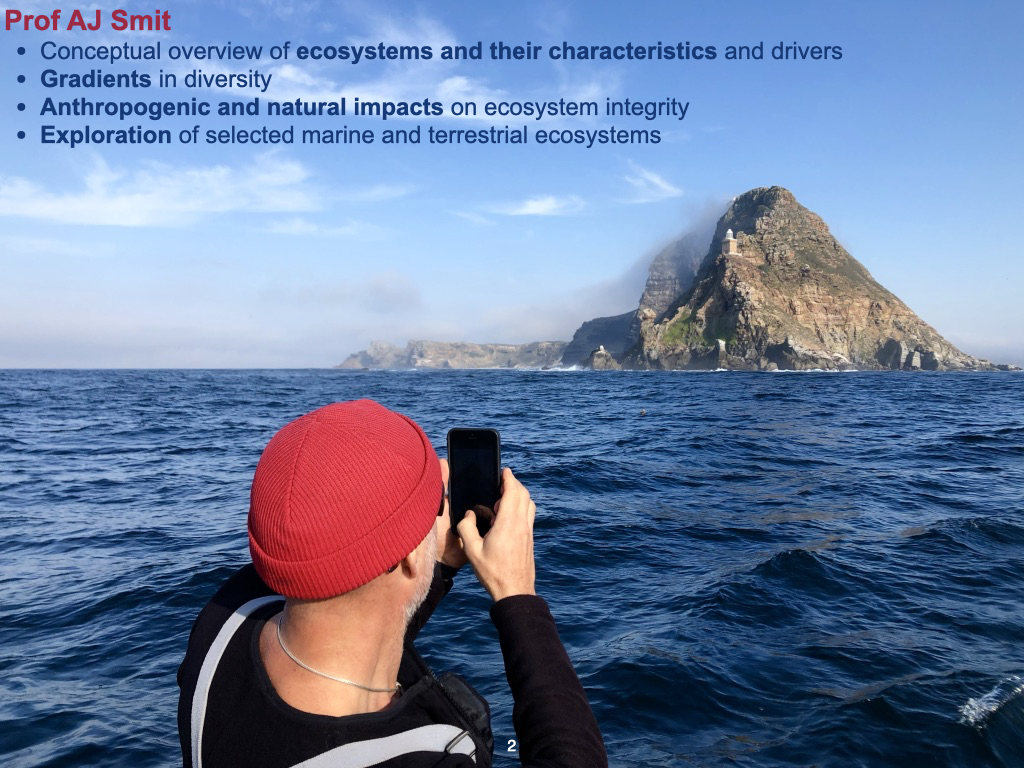
\includegraphics[width=0.8\linewidth]{../images/BDC334/BDC334-002.jpeg}
\caption*{Slide 2}
\end{figure}

So, we're going to look at a conceptual overview of what ecosystems are,
their characteristics, and what makes ecosystems work (Slide 2). An
ecosystem is easy to observe when you go out into nature; what you see
is, indeed, an ecosystem. However, they're present because something
explains their existence at a particular place and time. These are the
environmental factors that drive them, support their operation, and
allow them to function.

\section{Environmental Gradients and
Biodiversity}\label{environmental-gradients-and-biodiversity}

We'll discuss the broad concept of gradients in biodiversity, which is
important for you to consider. You need to think about all the gradients
in abiotic variables that exist across the surface of the planet. An
obvious example of a gradient is the one that exists from the tropical
regions at low latitudes to the high latitudes, the polar regions.

As we move from the tropical regions towards the polar regions, it
becomes progressively colder. The day length, or the ratio between day
and night, changes significantly, and the seasonal effect becomes more
pronounced. The amount of light decreases, and so on. There are many
different factors that vary along these large gradients from tropical to
polar regions.

There are also similarly strong gradients that exist on local scales.
For example, looking at Cape Point, there's a very strong gradient in
temperature as we move from the western side of Cape Point, around Cape
Point, and into False Bay; as you move, the temperatures become
increasingly warmer. That's a gradient that exists on a small spatial
scale, but you also have global scale gradients.

The intention of macroecology is to understand how ecosystems are
structured along these gradients.

\section{Ecosystem Structure and Human
Influences}\label{ecosystem-structure-and-human-influences}

We'll also discuss what it means for an ecosystem to have structure. As
we've just spoken about gradients, most of these are natural gradients.
However, there are also anthropogenic gradients --- human impacts or
factors. These are things that people do which cause ecosystems to
change, affecting how they function and how they're structured.

To demonstrate these various principles, we'll explore a selection of
the more interesting and important ecosystems on the planet, and I'll
leave it to you to decide which ones you find most interesting. You'll
have the opportunity to explore some of your own ecosystems, looking at
them in terms of both anthropogenic impacts and the natural influences
that make them different from other ecosystems. We'll investigate some
of the more important gradients responsible for structuring ecosystems
and examine their characteristics in terms of biodiversity, structure,
form, and so on.

\section{Course Structure: Professor
Boatwright}\label{course-structure-professor-boatwright}

\begin{figure}[ht]
\centering
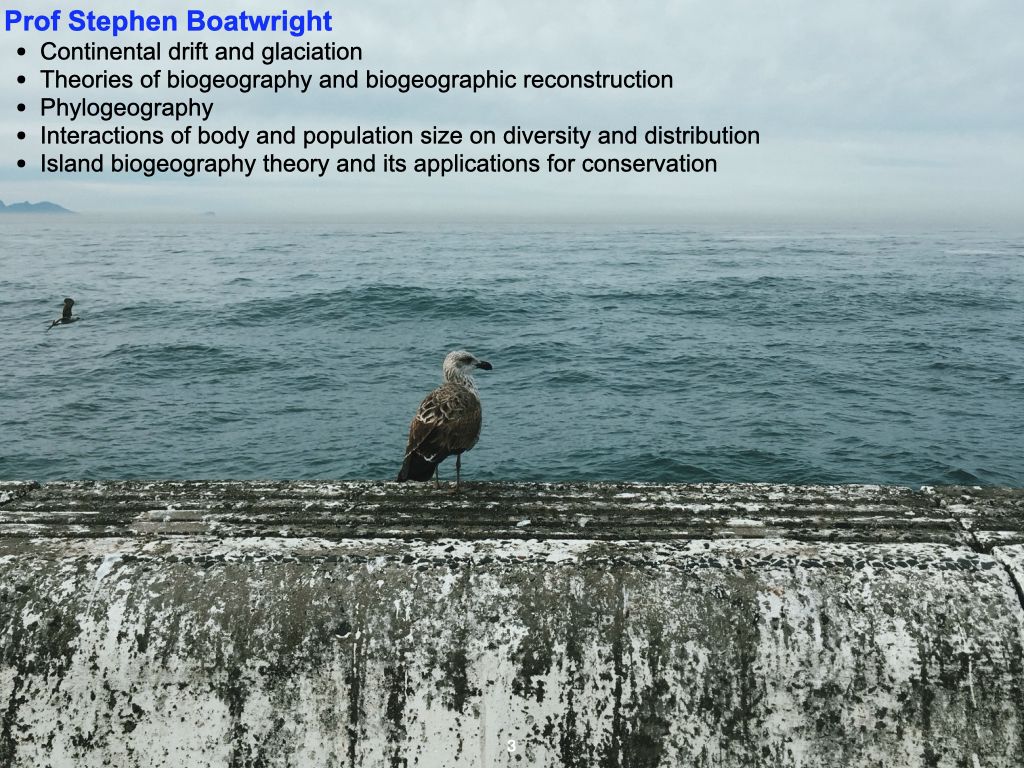
\includegraphics[width=0.8\linewidth]{../images/BDC334/BDC334-003.jpeg}
\caption*{Slide 3}
\end{figure}

Professor Boatwright will take over in the fourth term. He will cover
other aspects of macroecology and global ecology, including subjects
like continental drift and glaciation (Slide 3). This will involve
looking back into the palaeohistories of Earth, so his emphasis will be
more historical, whereas my emphasis will be on contemporary processes
and those we anticipate in the future. In fact, we can state with a
great deal of confidence --- up to perhaps about \(100\) years, possibly
\(150\) years --- what the future climate, temperature, and other
variables on Earth will likely be. Because ecosystems respond to changes
in these factors over such time scales, we can also infer the future
biogeography and macroecology of systems.

Professor Boatwright will also delve into phylogeography, which deals
with the genetic lineages of different forms of life across Earth's
surface, and how these are structured as a consequence of continental
drift and glaciation. He will further explore current patterns in body
size and population size as related to biodiversity and distribution.
Lastly, he will cover the theory of island biogeography.

\section{Gradients Beyond Earth}\label{gradients-beyond-earth}

\begin{figure}[ht]
\centering
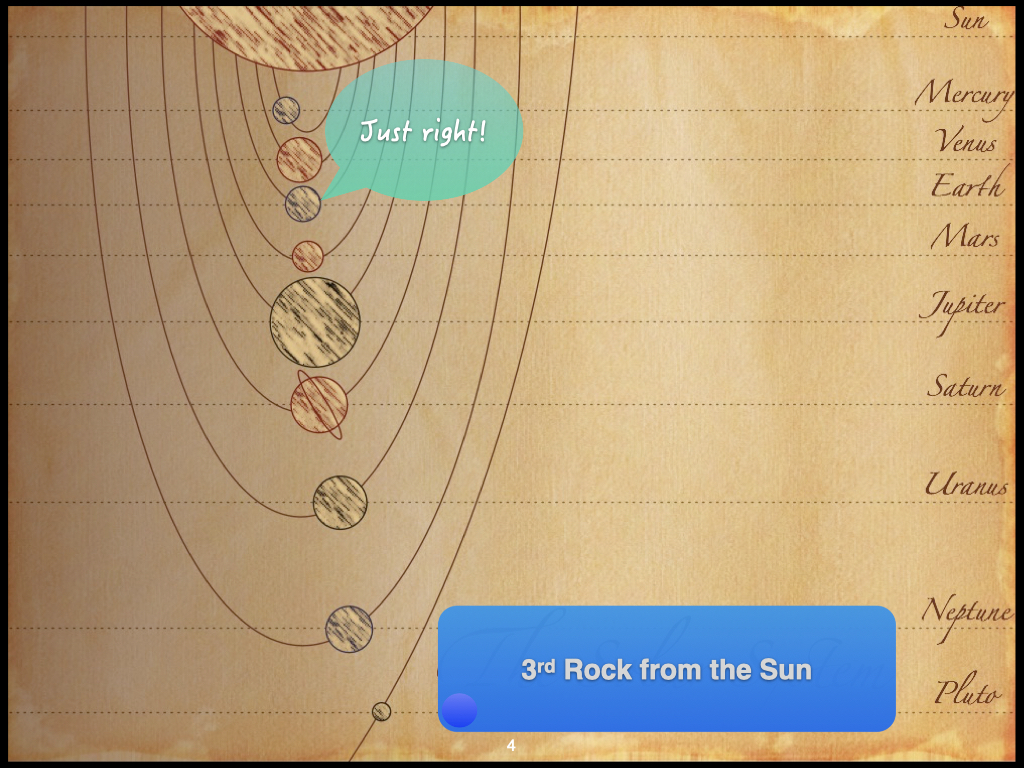
\includegraphics[width=0.8\linewidth]{../images/BDC334/BDC334-004.jpeg}
\caption*{Slide 4}
\end{figure}

Those gradients I mentioned also exist on much larger scales --- outside
of Earth itself (Slide 4). For instance, consider the arrangement of all
the various planets from Mercury, Venus, Earth, Mars, and so on. As you
move farther away from the Sun, it's not necessarily that it becomes
colder immediately, but the amount of heat available becomes less and
less. At a certain distance from the Sun, we find Earth, where the
conditions are just right for water to exist as a liquid, as ice, and as
vapour in clouds.

Go closer to the Sun and you come to Venus, which is the second planet
from the Sun. There, it's too warm and no water is available at all.
Move a little further away and you reach Mars, the fourth planet from
the Sun, where it's a bit too cold, so most of the available water
occurs as ice. Progress even further and, on the distant planets, even
some elements typically gaseous on Earth exist as ice. This gradient in
the solar system --- a function of distance from the Sun --- is what
creates Earth's unique set of conditions that permit life, as it depends
on the presence of liquid water, ice, and vapour.

\section{Outline of Topics for This
Module}\label{outline-of-topics-for-this-module}

\begin{figure}[ht]
\centering
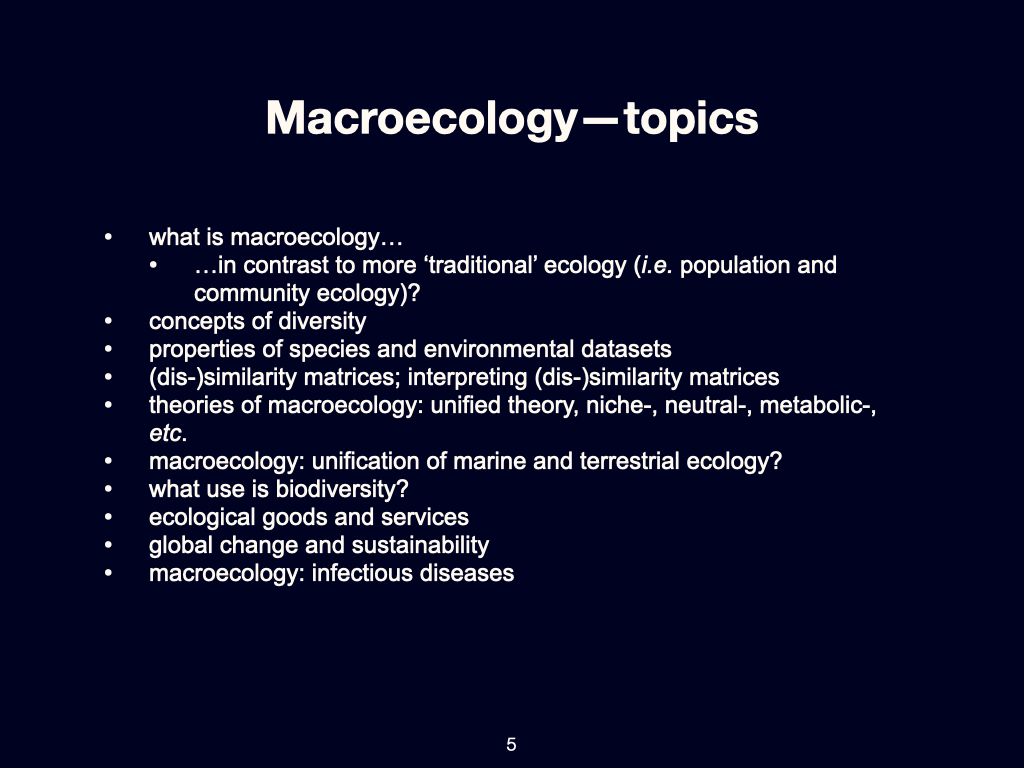
\includegraphics[width=0.8\linewidth]{../images/BDC334/BDC334-005.jpeg}
\caption*{Slide 5}
\end{figure}

In my section of the module, we will start by explaining what
macroecology is, contrasting it with more traditional approaches to
ecology (Slide 5). We will explore various concepts related to
diversity. Then, we will discuss how to do macroecology, which will
require us to examine some data and look at the properties of datasets
from which we can extract knowledge about how ecosystems are structured
in space and time, and how they function. To do this, we'll need to
understand some slightly mathematical concepts, including similarity and
dissimilarity matrices.

Later, we'll consider some unifying theories of macroecology. In recent
years, there has been a movement toward finding unifying explanations
for ecological patterns and processes on Earth. In the past, there were
collections of hypotheses for different situations, varying according to
organism size, the nature of the ecosystem, and so forth --- separate
theories for marine, aquatic, soil, terrestrial environments, etc. But
today, there is an interest in looking at all these aspects in an
integrated way.

Then, we will examine what biodiversity is, why it's important, and what
differentiates ecosystems with high biodiversity from those with reduced
diversity. We'll also look at the principles of biodiversity's value ---
the ``so what'' question --- by considering ecological goods and
services. What benefits do people derive from nature? Why does
biodiversity matter for us? Even if you do not live in a natural
ecological system --- because it's been transformed into, say, a
residential area --- you are still dependent on the wellbeing of natural
portions of Earth. If those landscapes lack biodiversity, people would
be far worse off.

\section{Looking into the Future and Broader
Applications}\label{looking-into-the-future-and-broader-applications}

We will then look to the future by considering global change and
sustainability. We will also see if we can find some parallels between
macroecology and infectious diseases, perhaps even try to understand
whether the COVID epidemic makes more sense given our knowledge of
macroecology.

\chapter*{Lecture 2b}\label{lecture-2b}
\addcontentsline{toc}{chapter}{Lecture 2b}

\section{Definition of Macroecology}\label{definition-of-macroecology}

\begin{figure}[ht]
\centering
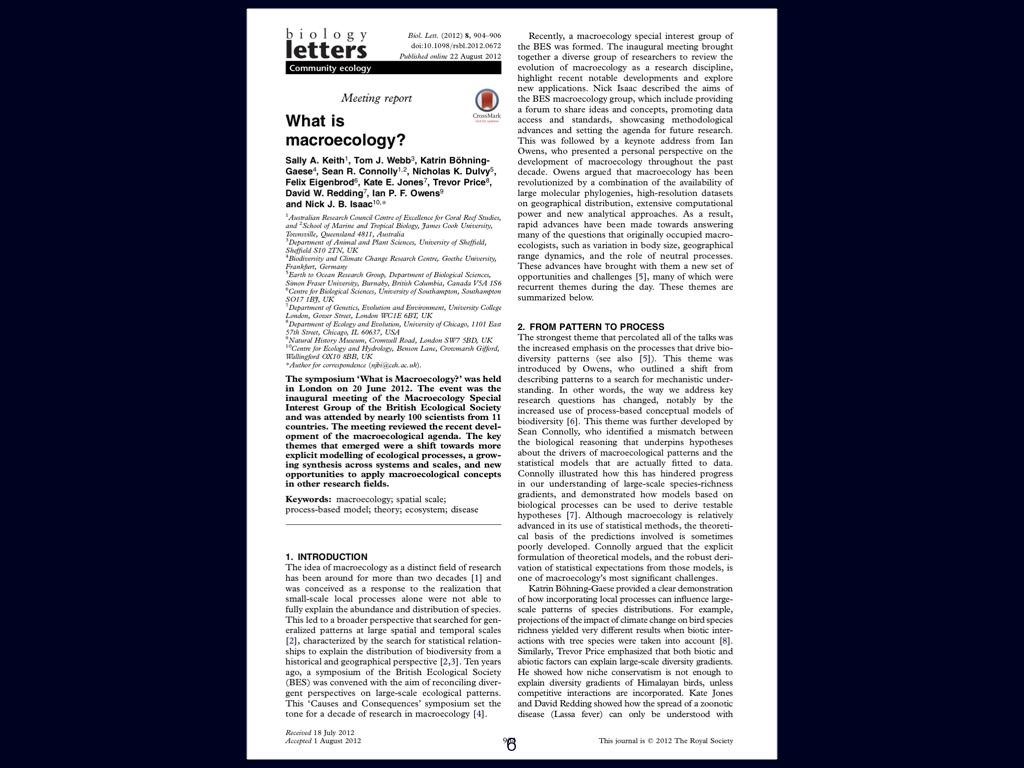
\includegraphics[width=0.8\linewidth]{../images/BDC334/BDC334-006.jpeg}
\caption*{Slide 6}
\end{figure}

\begin{figure}[ht]
\centering
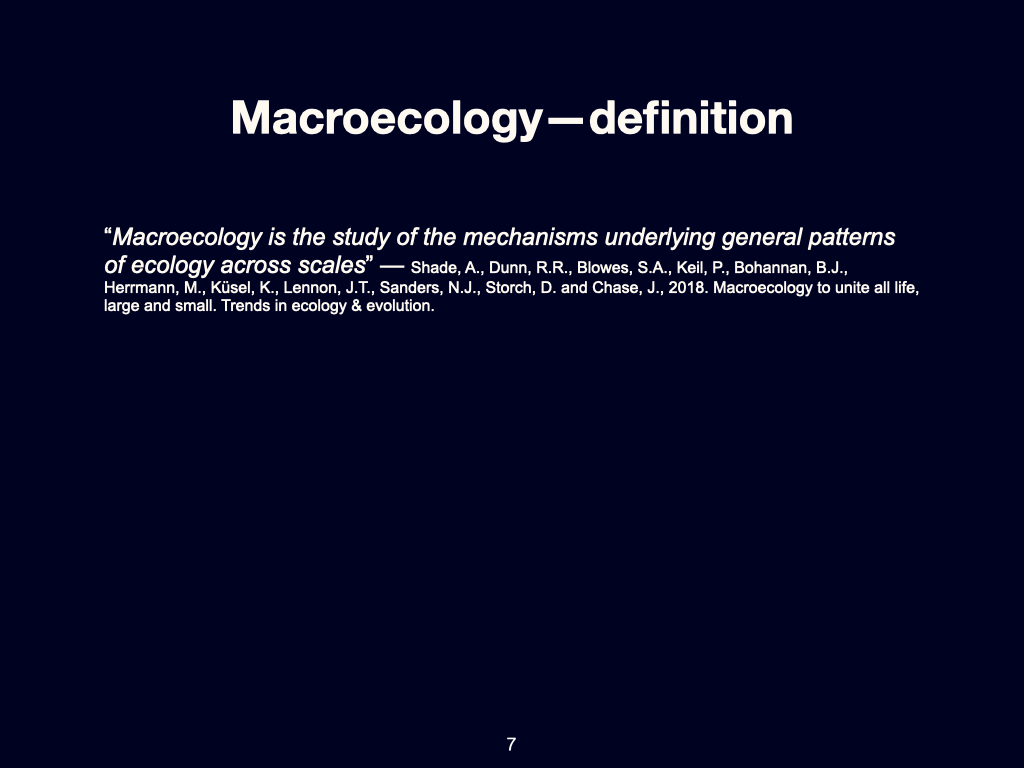
\includegraphics[width=0.8\linewidth]{../images/BDC334/BDC334-007.jpeg}
\caption*{Slide 7}
\end{figure}

I have already spoken a bit about this, but let me say a bit more. What
is macroecology (Slides 6-7)? If you were to summarise it in a sentence
or two, it is the study of the mechanisms underlying general patterns in
ecology, across scales. There are words there worth unpacking ---
`patterns' is probably one, and patterns in ecology across scales. The
two important ideas --- patterns and scales --- we'll be unpacking
further, if not today then in due course. I'll show you what
``patterns'' in ecological space can look like. But that's the essence
of macroecology.

Let's examine the definition in a little more detail.

\section{Traditional Approaches in
Ecology}\label{traditional-approaches-in-ecology}

\begin{figure}[ht]
\centering
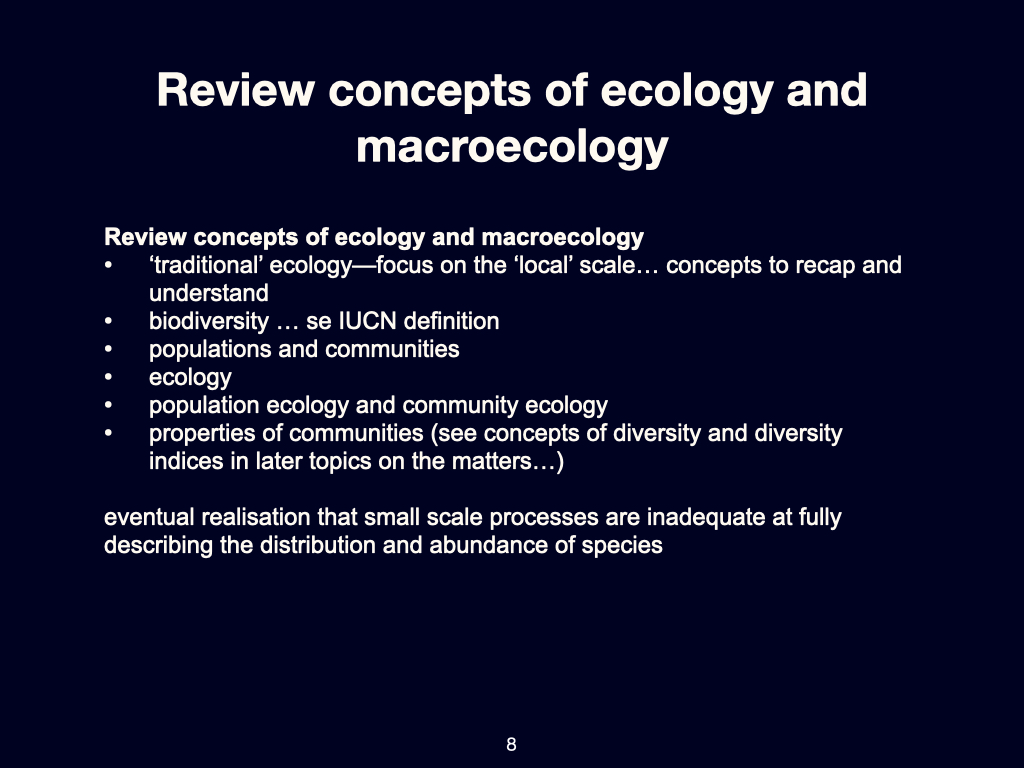
\includegraphics[width=0.8\linewidth]{../images/BDC334/BDC334-008.jpeg}
\caption*{Slide 8}
\end{figure}

To understand macroecology, you first need to understand how ecology has
traditionally been practised (Slide 8). Going back perhaps a hundred
years or more, even to Darwin's era, ecology was about observing and
investigating individual species. That is, the study of populations ---
a collection of individuals of the same species, occupying a specific
space and time. The focus was to examine the dynamics of a species
within a population: how it is affected by the environment, by other
species sharing the same space, and so on. Traditional ecology, then,
was very local in scale --- limited to what you could see, for instance,
standing at Cape Point and surveying the kelp forest before you. The
boundaries of that study would be as far as your eye could discern the
kelp --- very much a local scale.

But this ignores that kelp occurs not only at Cape Point, but also in
Norway, Iceland, and elsewhere worldwide. Macroecology would look at
kelp not only in South Africa, but also Norway, Iceland, the United
States, Canada, and everywhere kelp occurs. The aim is an integrated
understanding of the processes that make kelp forests work, regardless
of whether they are found in South Africa or New Zealand. Traditional
ecology, by contrast, kept its focus strictly local.

Now, due to advances in technology, data processing, and the sorts of
questions we're able to ask, the scope --- the scale --- of our enquiry
has greatly expanded. Today, macroecology can examine patterns at the
global level. Darwin embarked on a voyage round the world in the Beagle,
observing numerous locales --- it took him two, perhaps three years.
Today, in just \(24\) hours, we can obtain a `snapshot' of the entire
Earth and collect sufficient ecological data world-wide, something
previously unimaginable {[}attention: Darwin's ability to analyse global
ecology in a single synthesis was much more limited than described
here{]}. Thus, new technologies have altered our perspective.

\section{Biodiversity: Definitions and
Scales}\label{biodiversity-definitions-and-scales}

\begin{figure}[ht]
\centering
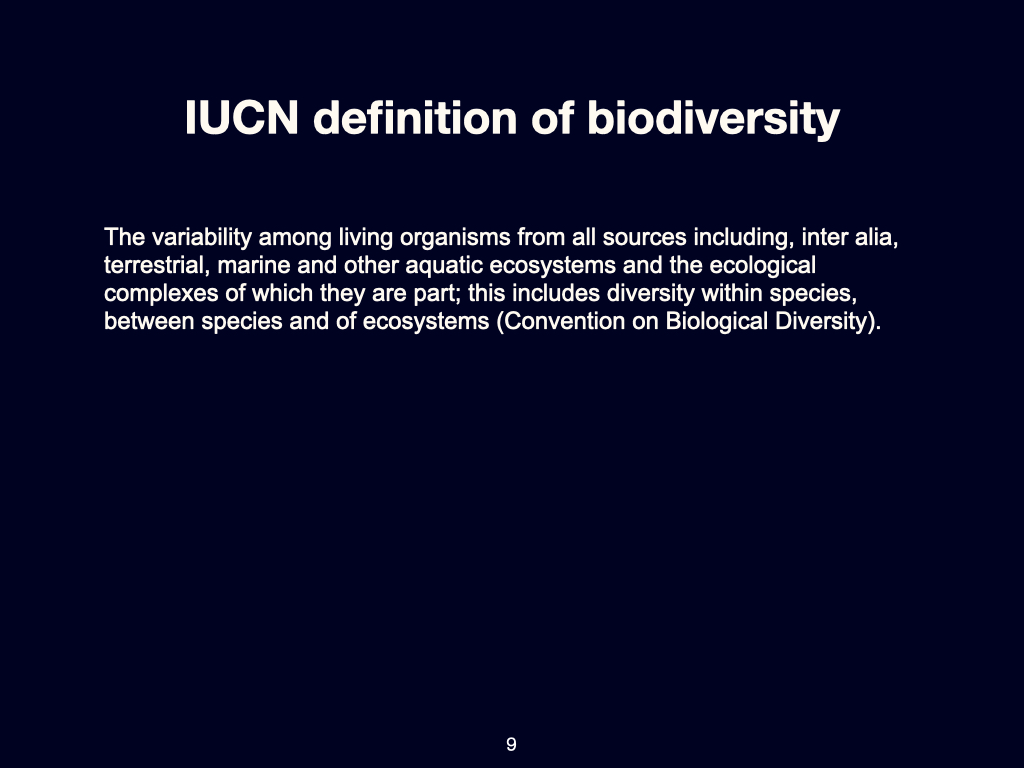
\includegraphics[width=0.8\linewidth]{../images/BDC334/BDC334-009.jpeg}
\caption*{Slide 9}
\end{figure}

Biodiversity is another key concept --- it appears throughout this
module, including in its very name. The traditional definition, as
described by the International Union for Conservation of Nature (IUCN;
Slide 9), defines biodiversity as ``\emph{the variability among living
organisms from all sources, including terrestrial, marine and other
aquatic ecosystems and the ecological complexes of which they are a
part. This includes diversity within species, between species, and of
ecosystems.}''

Again, the question of scale becomes evident --- diversity within
species, for example, means taking humans: within \emph{Homo sapiens}
there is great diversity, all the way down to genetic differences.
That's a scale we can go down to --- though Prof Boatwright will cover
genetics; I won't get into that aspect here.

Diversity also exists between species --- species occupying the same
ecosystem. In a kelp forest you might have \emph{Ecklonia maxima},
\emph{Laminaria pallida}, \emph{Macrocystis pyrifera}, various red
baits, fish, sharks, and so on --- all interacting within the kelp
forest. Then, there is diversity at the ecosystem level --- kelp forests
interact with pelagic ecosystems nearby, with the rocky shore, with
coastal dunes on the land, and so forth. Globally, a diversity of
ecosystems exists, each with its own species assemblages and modes of
environmental interaction.

So, biodiversity is essentially all life on Earth, at all the various
scales in which we observe it, and in all the different configurations,
forming habitats or ecosystems regardless of location --- from
\(11,000\,\mathrm{m}\) below the ocean surface to the summit of Mount
Everest.

\section{Populations, Communities, and the Move to
Macroecology}\label{populations-communities-and-the-move-to-macroecology}

So, we've mentioned populations (collections of one species) and
communities (collections of multiple species). Ecology studies the
processes by which species relate to their environment, to each other,
and how the environment influences both populations and communities.

Macroecology naturally starts from population and community ecology: it
makes sense to move from the local scale, to groups of communities, and
then ultimately to encompass the whole Earth, which is the domain of
global ecology and macroecology.

A proper understanding of the effects of scale, and of various scaling
processes and gradients --- as they occur from local to global levels
--- is absolutely crucial. This knowledge helps explain why certain
species exist in particular locales but not in others. For example, why
do kelp forests thrive in Cape Town, but not off Durban in
KwaZulu-Natal? It's because the environmental conditions differ: Cape
Town's seawater is much colder throughout the year, making it suitable
for kelp, while Durban's warmer temperatures exclude kelp from surviving
there.

Some organisms actually require kelp forests to survive or to reach
their full productivity --- certain species can only occur within kelp
forests. So, the presence of kelp creates an environment that supports
many other species. Thus, if kelp is absent (as off Durban), these
organisms are also absent.

In short, global ecology seeks to understand how variations in
temperature, light, soil characteristics, air quality, snow, rainfall,
drought, humidity --- all these environmental variables --- combine to
create a patchwork of suitable conditions for some species, but not
others. Ecology, and especially macroecology, attempts to find global
explanations for these broad patterns.

\section{Questions \& Answers}\label{questions-answers-1}

\begin{figure}[ht]
\centering
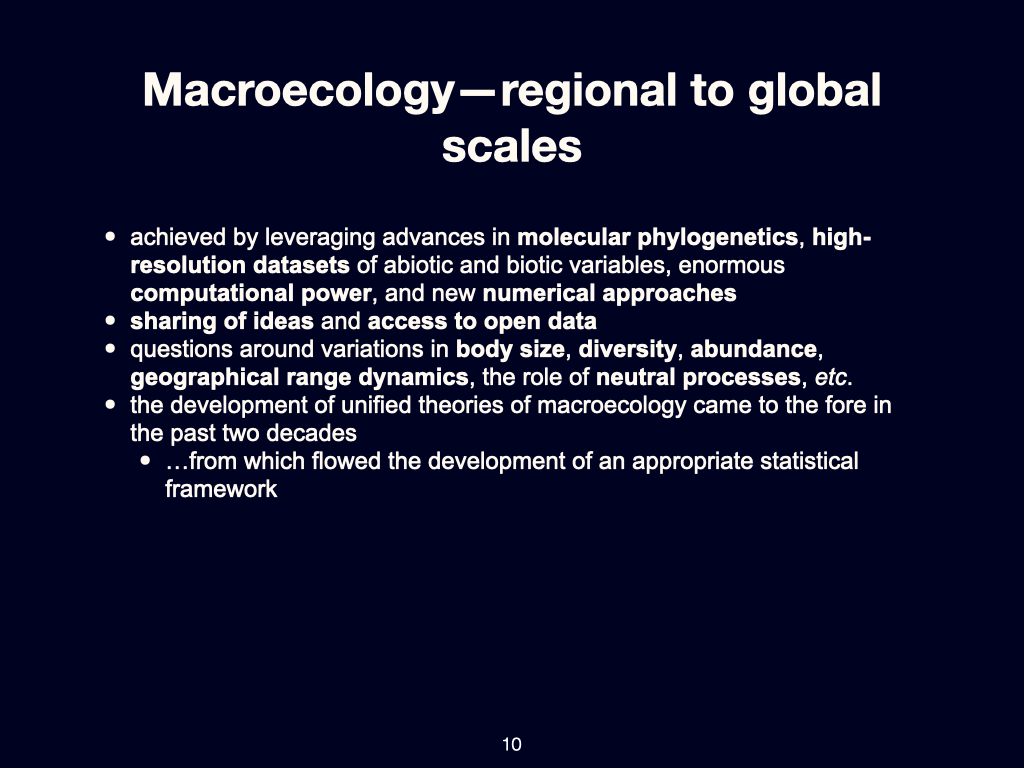
\includegraphics[width=0.8\linewidth]{../images/BDC334/BDC334-010.jpeg}
\caption*{Slide 10}
\end{figure}

A question arose: when referring to patterns and processes in
traditional ecology, is there such a thing as modern ecology? Yes, this
module is very much about modern ecology. Traditional ecological
approaches would focus on surveys at a local scale, such as conducting a
transect survey in a nearby nature reserve, limited by what can be
physically accessed.

Today, with computers and satellite remote sensing, we can examine
large-scale patterns --- across countries, continents, or even globally
--- often using satellite data (Slide 10). Not only can we synthesise
many small-scale surveys collected by different people over time, but we
can also employ advanced numerical analyses to make sense of very large
data sets --- ones so substantial, they can no longer fit within Excel.

Modern ecologists now collaborate across the globe, pool significant
data sets, and use advanced methods to reveal broad-scale patterns in
biodiversity, species composition, and ecological functioning. Whereas
traditional studies looked at the local, modern ecology can rigorously
address processes at global, continental, or deep historical time
scales.

\subsection{Example from South African Vegetation
Mapping}\label{example-from-south-african-vegetation-mapping}

For example, in the 1940s,
\href{https://en.wikipedia.org/wiki/John_Phillip_Harison_Acocks}{John
Acocks} (7 April 1911 -- 20 May 1979), attempted to classify all of
South Africa's vegetation. He travelled by train, classifying the
habitats he saw through the window, and his classification became known
as the \emph{Veld Types of South Africa}. Even this method was
constrained compared to the view we now have through remote sensing
satellites.

Now, we can stand ``\(80\,\mathrm{km}\)'' above the Earth and map entire
landscapes from above, unconstrained by natural or political boundaries.

\subsection{Broader Shifts in
Approach}\label{broader-shifts-in-approach}

Traditional ecological studies focused on what happens in places within
easy reach --- a single nature reserve, for example. Modern studies look
for patterns across nations or hemispheres, and also explore new levels
of taxonomic detail, such as genetic variation and subspecies.

`Scale' can refer both to spatial scale --- local to global --- as well
as temporal scale: considering recent changes versus millennia or longer
time spans. Modern approaches allow us to examine ecological phenomena
and biogeographic patterns at both these broader spatial and longer
temporal dimensions.

Collaboration is increasingly important. Where once ecological studies
might have one or two authors focused on a single location, it's now
common to find large teams of co-authors bringing together expertise and
data from multiple sites or even continents in pursuit of broader
ecological generalities.

\subsection{The Value of Global
Approaches}\label{the-value-of-global-approaches}

The aim of global ecology is to derive general ecological `laws' or
repeatable principles that apply across the full diversity of ecosystems
--- from Russian tundra to Amazonian rainforest to the Australian
outback. Though these systems may look entirely different, we seek to
identify commonalities in their fundamental processes.

Thirty years ago, when I was a student, almost all work was at a very
local scale and typically on one's nearest nature reserve. Today, with
advances in technology and computational power, questions can be more
complex and less parochial. The questions themselves have evolved and
broadened: ``What can South Africa's biodiversity teach Patagonian
ecologists?'' Global-scale studies provide answers of relevance far
beyond one region or ecosystem.

\subsection{Closing and Summary}\label{closing-and-summary}

If you have further questions --- about the module structure,
assessments, or the content of the introductory material --- please ask,
either now or later via the chat or WhatsApp group.

If there are no more questions, I'll post this video online for you to
access within the next half an hour or so. Thank you.

\chapter*{Lecture 2c}\label{lecture-2c}
\addcontentsline{toc}{chapter}{Lecture 2c}

\section{Revisiting Definitions and
Scales}\label{revisiting-definitions-and-scales}

Regional to global scales --- I've spoken about all of this already, so
I don't need to go into regional to global scales again. You'll
understand this in a little bit more detail once you read that paper
that I've given you. There are going to be two other papers now which
you're expected to read as well.

\section{Patterns and Processes}\label{patterns-and-processes}

\begin{figure}[ht]
\centering
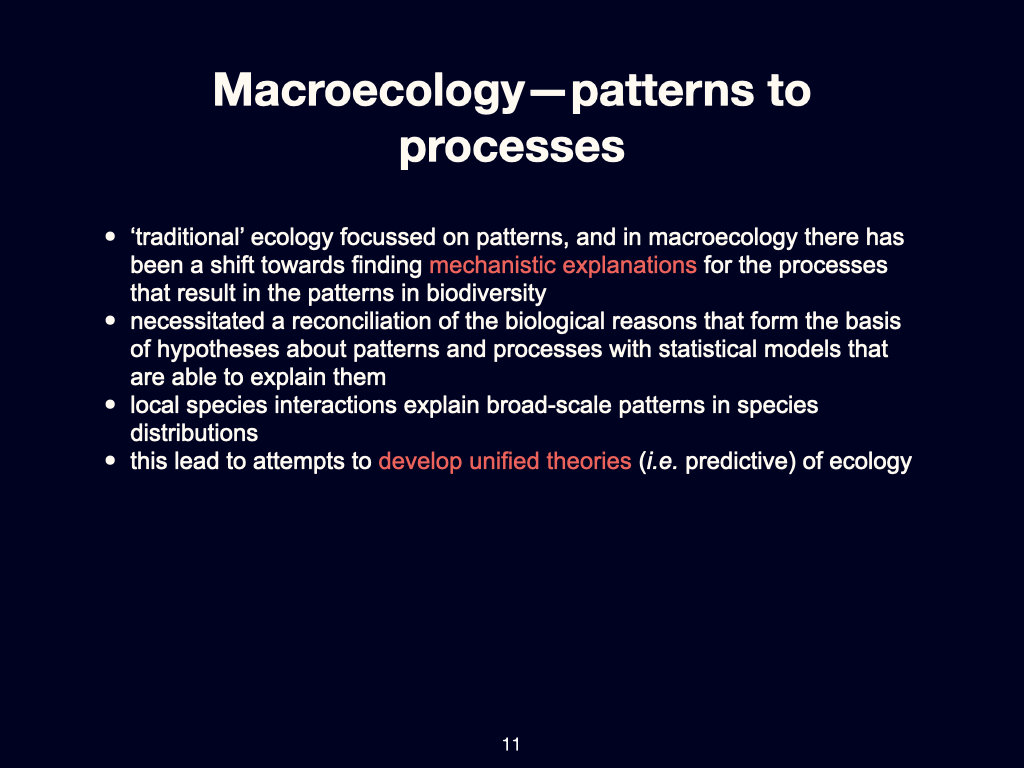
\includegraphics[width=0.8\linewidth]{../images/BDC334/BDC334-011.jpeg}
\caption*{Slide 11}
\end{figure}

Okay, patterns and processes (Slide 11). Traditional ecology essentially
focused on patterns. It looked at the world and observed that there is a
patchwork of different kinds of ecosystems, even on local scales and
then regional scales. It noted that this ecosystem often appears
different from the one next door, and described how it is different in
terms of species present there, and in terms of the structure of the
community. However, it didn't really attempt to explain the mechanism
that created those differences in the first place.

In contrast, macroecology tries to add a mechanistic explanation for why
and how things differ across the surface of Earth. To do this, we need
to start treating ecology as a proper science, not merely as a form of
natural history as it had been approached in the past. We need to ask
questions about nature, to form hypotheses about nature that can be
tested statistically, so that we can have a cause--effect explanation
for why things are the way they are, or how things came to be as we
observe them now.

This is, in fact, a very critical feature of modern-day ecology,
particularly in macroecology, but also in contemporary population and
community ecology at the local scale. We must ask testable hypotheses
about nature --- questions that we can actually go and test
experimentally. Experimental assessment, experimental science, is the
true test for whether something is so, or is not so. The necessity to
measure things, and the necessity to have a statistical model or
hypothesis, requires that we have data --- that we go out into the world
and measure things in specific ways, in order to have data that can be
tested in a hypothesis setting via statistical models.

This is a very key part of modern ecology, and it's only something that
has become feasible since about the 1970s. Before that, people did not
look at ecosystems with the intention of asking hypotheses of them. They
mostly described how things are, rather than why things became the way
we observe them to be now.

\section{Local Interactions to Global
Theories}\label{local-interactions-to-global-theories}

We're going to examine local species interactions all the way up to
global species distributions. Hence the necessity, once we have the
entire earth in view, to develop unified theories. There are, of course,
various applications.

\section{So What?}\label{so-what}

\begin{figure}[ht]
\centering
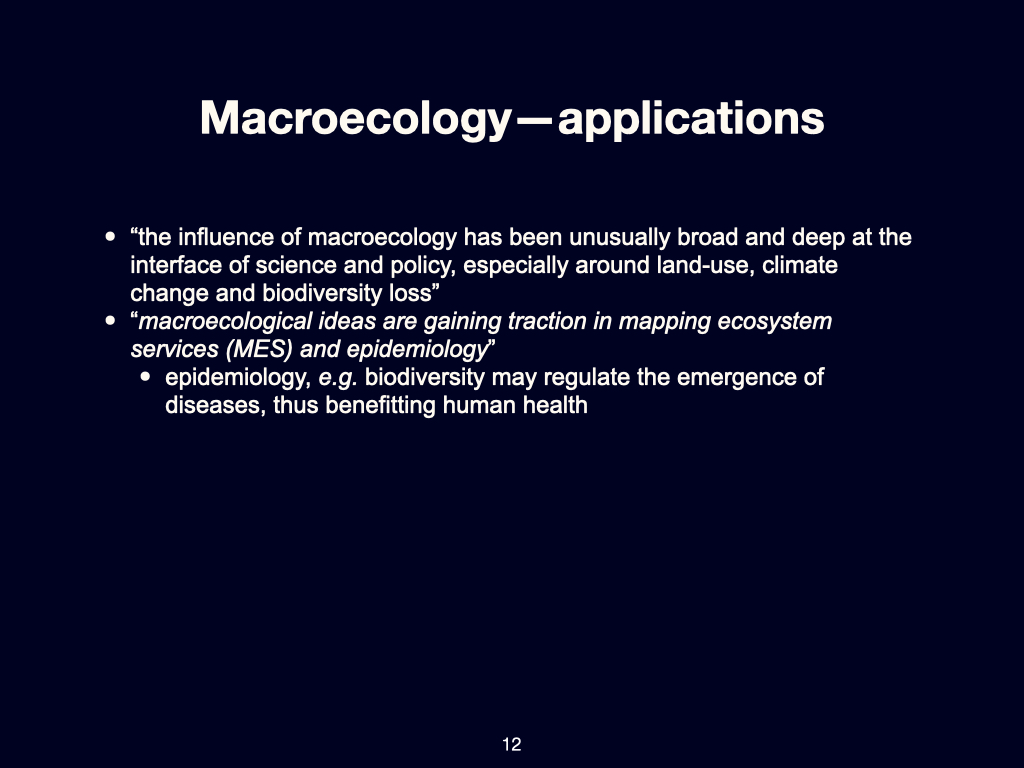
\includegraphics[width=0.8\linewidth]{../images/BDC334/BDC334-012.jpeg}
\caption*{Slide 12}
\end{figure}

Why do we want to do macroecology (Slide 12)? Because we want to create
something for policymakers to help them understand the world better; to
identify that certain regions of the world are of great importance, both
strategically and ecologically, and for the benefit of people. It may be
better not to have developments in such areas, or instead to conserve
portions of biodiversity, to plan land use accordingly, and to
understand what the future world is likely to be like as biodiversity is
lost to an ever-greater extent.

So, understanding macroecological processes influences the way that
policies unfold. One of the major visible policies in the world today is
the tendency for nations to move away from fossil fuels towards
renewable energy, because we know that fossil fuels cause climate
change, and we know that climate change is having an effect on species
globally. We want to minimise this effect, because if we do, the
consequences for people will also be reduced, since humans are so
strongly linked to the environment.

Additionally, explanations of epidemiology also become possible:
understanding the ways in which diseases spread and operate around the
world, their origins, and so forth. There are many reasons why
macroecology is interesting and important. For me, it is important
because people are making a living from the world around us, and we want
to ensure that the way people are making a living from the world today
will still be viable a century from now --- for your children, perhaps,
to make a similar kind of living from the world, if you indeed directly
rely on natural systems. Even if you don't directly depend on
ecosystems, you are indirectly supported by ecological goods and
services.

\section{Self-Study and Assignments}\label{self-study-and-assignments}

\begin{figure}[ht]
\centering
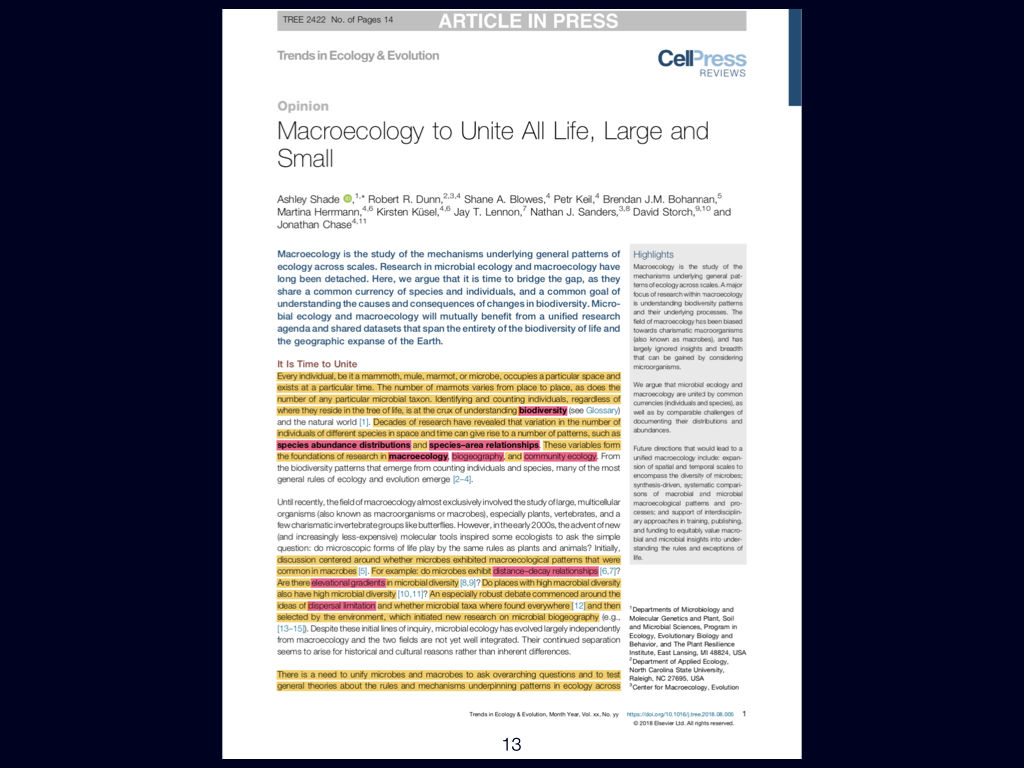
\includegraphics[width=0.8\linewidth]{../images/BDC334/BDC334-013.jpeg}
\caption*{Slide 13}
\end{figure}

\begin{figure}[ht]
\centering
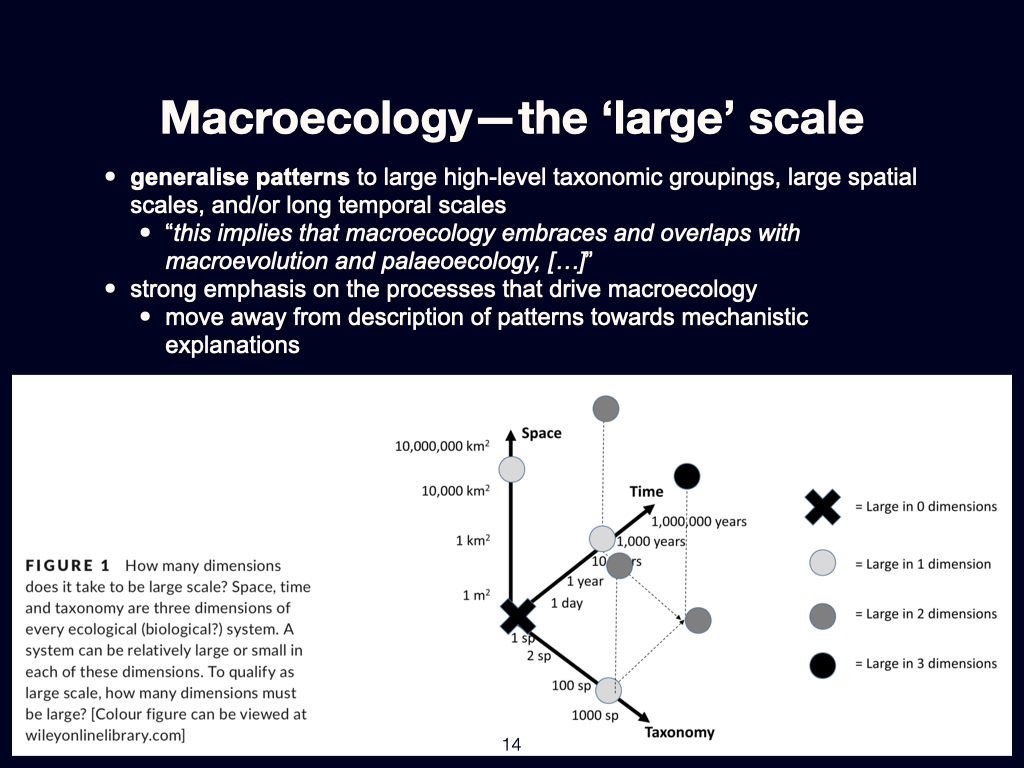
\includegraphics[width=0.8\linewidth]{../images/BDC334/BDC334-014.jpeg}
\caption*{Slide 14}
\end{figure}

Anyway, that brings me to the end of what I needed to say today. There
are two papers --- or rather, one paper and one additional paper (Slides
13-14). There's the one you saw before, and another one, which is also
available to download from Tangled Bank. I would like you to read them
both by the end of this week, so that by Friday afternoon, if you have
questions about them, you can ask me. I'll be available on Google Meet
if you make an appointment to see me in groups of more than three.

So that's your self-study. Your assignments will also require that you
understand these topics in quite a bit of detail.

\section{Looking Ahead}\label{looking-ahead}

During the next lecture, we shall move on to topic number two, and we're
going to look at some of the questions that we can ask within the
framework of macroecology.

\chapter{Ecological Gradients}\label{ecological-gradients}

\begin{tcolorbox}[enhanced jigsaw, colback=white, bottomrule=.15mm, opacitybacktitle=0.6, arc=.35mm, opacityback=0, left=2mm, coltitle=black, colframe=quarto-callout-note-color-frame, breakable, bottomtitle=1mm, toptitle=1mm, toprule=.15mm, titlerule=0mm, leftrule=.75mm, title=\textcolor{quarto-callout-note-color}{\faInfo}\hspace{0.5em}{BCB743}, colbacktitle=quarto-callout-note-color!10!white, rightrule=.15mm]

This material must be reviewed by BCB743 students in Week 1 of
Quantitative Ecology.

\end{tcolorbox}

\chapter*{Lecture 3a}\label{lecture-3a}
\addcontentsline{toc}{chapter}{Lecture 3a}

\section{Papers to Read}\label{papers-to-read-1}

The next paper you need to be familiar with addresses the `distance
decay' phenomenon. It is by Nekola and White (1999). This paper links
directly to concepts introduced in the previous Ashley Shade paper, but
here it is explored in greater detail.

The distance decay relationship fundamentally explains how ecological
similarity decreases with geographical or environmental distance. In my
view, gradients---particularly environmental gradients---are the major
structuring agents of life on Earth, and distance decay is the pattern
that emerges when we observe biodiversity at broad, often global,
scales.

Zooming in to finer spatial scales, randomness or stochasticity becomes
more influential, and the structure of beta diversity becomes more
complex. Specifically, the paper introduces concepts such as turnover
beta diversity and nestedness resultant beta diversity. If you find
these terms challenging or require deeper understanding, you should
consult foundational works by Whittaker and Baselga, who have written
extensively on these topics. Understanding both nestedness resultant and
turnover beta diversity is essential for your overall grasp of the
subject.

This paper by David Tilman (2017) explores global-scale environmental
gradients and their explanatory power in patterns of biodiversity. It
specifically delves into the mechanisms underlying global patterns,
focusing on the marine environment.

You are expected to understand the unimodal species distribution model,
as it underpins the interpretation of distance decay across
environmental gradients. While one group will further explore
terrestrial patterns of biodiversity as part of the wiki assignment,
this particular paper gives a clear overview for marine systems. Pay
special attention to the graphs presented, as these summarise the major
explanatory patterns in a digestible format.

\section{Macroecology and Environmental
Gradients}\label{macroecology-and-environmental-gradients}

\begin{figure}[ht]
\centering
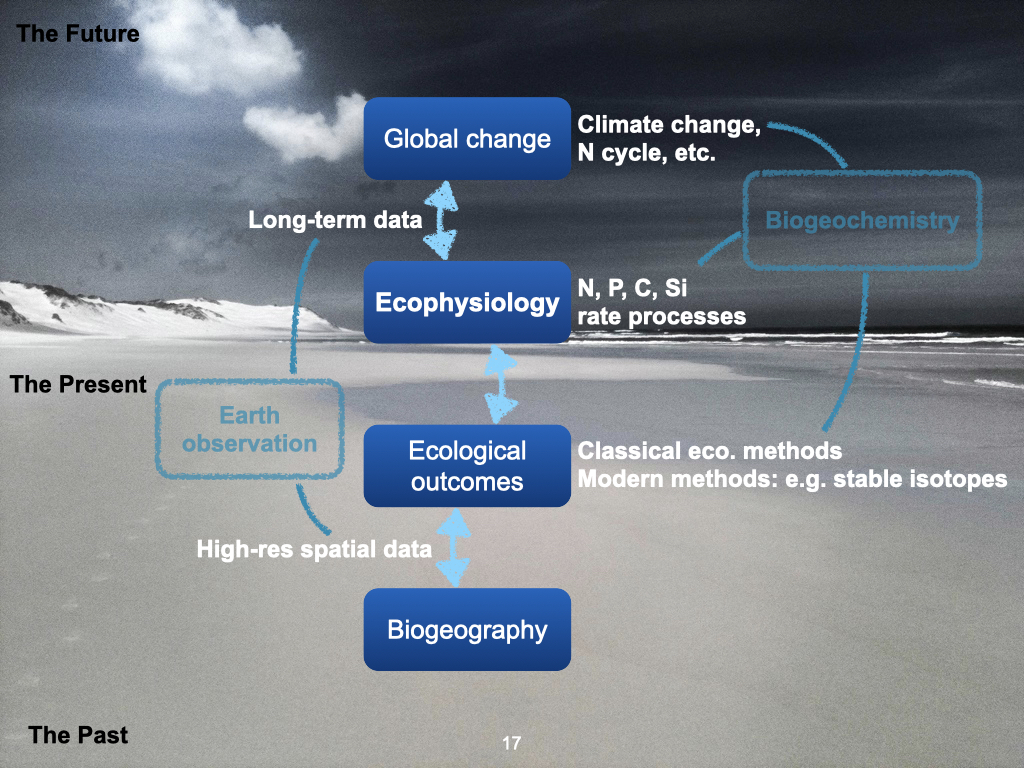
\includegraphics[width=0.8\linewidth]{../images/BDC334/BDC334-017.jpeg}
\caption*{Slide 17}
\end{figure}

We are starting with topic number two in biogeography and global
ecology. Today, our discussion focuses on the effect that gradients ---
specifically, environmental gradients --- have on the distribution of
life across the planet (Slide 17).

To remind you what macroecology is concerned with, we can use it to ask
almost any question about the biodiversity of life on Earth. More
specifically, we explore how biodiversity is arranged according to
geographical location. This pertains to differences between continents,
across continents, and indeed, across the entire Earth. Our scope is
broad: we consider patterns found on very small, local scales right here
around us, scaling up to global patterns that encompass the whole
planet.

Moreover, macroecology allows us to look deep into the past, using
palaeorecords to explore the distribution of plants, animals, and also
organisms that are neither plant nor animal. Equally, it grants us tools
to study what is happening right now, in the present day. Looking to the
future is also now possible due to technological advancements, such as
computational modelling and remote sensing.

For my particular section of the module, as I mentioned yesterday, we
are focusing mainly on contemporary processes. We will also look, albeit
briefly, at methodologies for measuring these distributions and at how
we establish the patterns of distribution for both plants, animals, and
other organisms globally.

\section{Drivers of Biogeographical
Patterns}\label{drivers-of-biogeographical-patterns}

Let's firstly examine the processes present around us that structure the
global distribution of life. The way we currently observe life arranged
at the global scale is termed `biogeography'.

Generally speaking, biogeography and the biodiversity patterns
associated with different continents and regions depend largely upon the
underlying geographical character of those regions. Climate is an
important factor here --- it has a substantial, direct influence on
these patterns.

However, it is crucial to appreciate that the deeper history, or
palaeohistory, of Earth also matters. The original evolution of life,
and, long ago, the manner in which today's continents were previously
joined into supercontinents --- initially Pangaea and, subsequently,
Gondwana --- are instrumental in explaining our current patterns. The
break-up of these supercontinents, driven by plate tectonics, has
critically shaped the biological structures we observe across the
planet's surface today.

\section{Remote Sensing and Modern
Observation}\label{remote-sensing-and-modern-observation}

These processes are not just theoretical; we can observe and quantify
them. We have access to high-resolution spatial data, much of it
obtained from satellites that orbit Earth daily. Since roughly \(1981\)
--- the beginning of what we call the satellite era --- we have been
able to compile global images of Earth's surface. This has enabled an
unprecedented understanding of patterns and processes relating to
terrestrial life.

Environmental differences across the Earth's surface produce varying
ecological structures and outcomes. These outcomes, meaning both the
structure and function of ecosystems, depend on --- and can be measured
across --- different places and environments on our planet.

\section{Classical and Modern Ecological
Methods}\label{classical-and-modern-ecological-methods}

Classical ecological approaches --- such as population and community
ecology --- have, for the last hundred years or so, helped elucidate how
such ecological patterns develop and persist. These approaches include
basic methods such as sampling using quadrats or transects, with
researchers counting the number of different species co-existing in
defined areas, and then tracking how these assemblages vary both
spatially and temporally.

You should recall from your earlier studies the relationship between
plants, animals, and their environment, particularly regarding how the
environment acts upon the physiology of specific organisms.

\section{Linking Environment, Physiology, and
Ecology}\label{linking-environment-physiology-and-ecology}

Furthermore, macroecological questions encompass the many rate processes
that move major nutrients --- such as nitrogen, phosphorus, and carbon
--- as well as both micronutrients and macronutrients, into and away
from plants and animals. These environmental influences on living
organisms can be measured in a field known as ecophysiology. This
discipline examines the rate processes affecting both plants and
animals: for plants, things like nutrient uptake, and for animals,
factors such as prey capture or their movement capabilities, as
discussed previously by Prof Maritz All these variables are studied
within ecophysiology.

Importantly, outcomes from ecophysiological processes can have broad
ecological consequences. That is, changes at the level of organismal
physiology often scale up to influence community structure and even
biogeographical patterns.

\section{Global Change: Past, Present, and
Future}\label{global-change-past-present-and-future}

Finally, we must recognise that the world, at all levels, is being
transformed by global changes, including shifts in climate, and in
nutrient cycles --- such as those for nitrogen and phosphorus. This
revisits topics from your Planetary Boundaries lectures in second year.
Global change will influence --- and in many cases, is already
influencing --- the outcomes of ecophysiological processes, which
translate upstream to affect ecological patterns and, eventually,
broad-scale biogeographical distributions.

To summarise, all these various processes --- ranging from global
change, through ecophysiology and ecological outcomes, to biogeography
--- occur across a huge variety of scales, both spatially (from the
entire Earth down to highly local settings) and temporally (from the
deep past, through the present, and projecting into the far future).

These are the foundational perspectives you should keep in mind as we
proceed.

\chapter*{Lecture 3b}\label{lecture-3b}
\addcontentsline{toc}{chapter}{Lecture 3b}

\section{Environmental Gradients}\label{environmental-gradients}

We have previously discussed gradients, particularly environmental
gradients. When I refer to gradients, I mean the changes in an
environmental variable, such as temperature or rainfall, as you move
from one place to another. For example, consider the temperature
difference between Johannesburg and Cape Town, or the rainfall
difference as you move from Durban to Cape Town. As you travel across
the land surface, you experience a gradient.

A prominent example is the rainfall gradient as one moves from east to
west across South Africa. KwaZulu-Natal, on the eastern side, is very
wet, with high rainfall and high humidity. However, as you move
westwards, into the Western Cape, the Northern Cape, and even further
towards Namibia, the environment becomes increasingly dry and
desert-like.

On the eastern side of the country, the climate is very wet, and thus we
find plants and animals that are adapted to, and require, very wet and
moist conditions --- examples include tropical or subtropical forests
and coastal forests. However, if you think back to the last time you
drove from Durban into the Northern Cape, you would have noticed how the
landscape became increasingly dry. As you continue across the landscape,
the vegetation also changes. It shifts towards types of vegetation that
are able to persist and thrive under quite dry conditions.

In the Northern Cape and further west towards the South African coast,
vegetation becomes increasingly sparse. There are fewer plants present
--- not necessarily fewer species, but rather, the individuals are far
more separated from each other in space. They are less dense, in other
words. This provides an example of a gradient related to rainfall, or
water availability.

\section{Environmental Gradients}\label{environmental-gradients-1}

Each different environmental variable can constitute a gradient.
Gradients occur for temperature, humidity, soil nutrients, soil
characteristics, cloud cover --- essentially, anything you can think of
regarding the environment. All these gradients operate across the
earth's surface.

Let us focus, for instance, on plant species. An individual species of
plant will often be well-adapted to a particular, relatively narrow,
range of environmental conditions --- such as temperature. Most
individuals of a given species tend to occur around a `sweet spot' where
conditions, such as temperature, are most comfortable for them.

To put this in more relatable terms, if you are in Cape Town on a sunny
summer's day, you will naturally gravitate towards the spot that is most
comfortable, perhaps choosing to sit in the shade rather than the direct
sun. Plants, of course, lack the ability to move from place to place as
we do. They are fixed in position, but over evolutionary timescales,
both plants and animals become most abundant where environmental
conditions are the most suitable for them.

\section{The Unimodal Response}\label{the-unimodal-response}

\begin{figure}[ht]
\centering
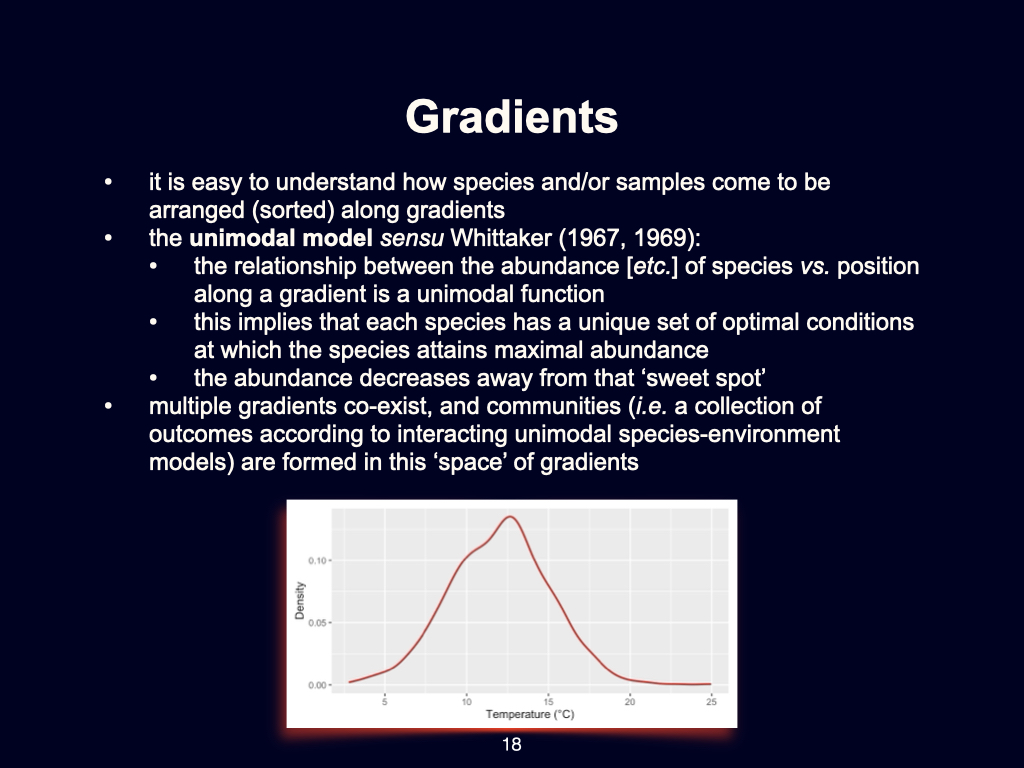
\includegraphics[width=0.8\linewidth]{../images/BDC334/BDC334-018.jpeg}
\caption*{Slide 18}
\end{figure}

Consider the example of a graph displaying the abundance of a particular
species in relation to temperature (Slide 18). For instance, the
majority of a species' individuals may be found where the temperature is
around \(12.5~^\circ\text{C}\), as that is the most suitable value for
them. As you move away from that optimal temperature, the abundance of
individuals decreases. This general pattern of abundance along an
environmental gradient is known as a `unimodal' species distribution.

You may read more about the origins of this concept in the work of Roger
Wittig {[}attention: likely incorrect, please verify author and
publication details{]} from 1967 or 1969, where this idea of the
unimodal species distribution was first discussed.

Of course, this applies only to one particular species. A different
species may have an optimal temperature around \(20~^\circ\text{C}\),
others at \(5~^\circ\text{C}\); some will prefer lower, some higher, and
so on. These preference curves exist for every single environmental
gradient and for all species present.

\section{Gradients Beyond
Temperature}\label{gradients-beyond-temperature}

It is important to recognise that this pattern is not restricted to
temperature. The same kind of unimodal distribution occurs for gradients
in humidity, water availability, soil type, nutrient concentration, and
other factors that have ecological or physiological consequences for
species.

When those factors operate simultaneously, they result in complex
patterns known as coenoclines.

\section{Coenoclines, Coenoplanes, and
Coenospaces}\label{coenoclines-coenoplanes-and-coenospaces}

\begin{figure}[ht]
\centering
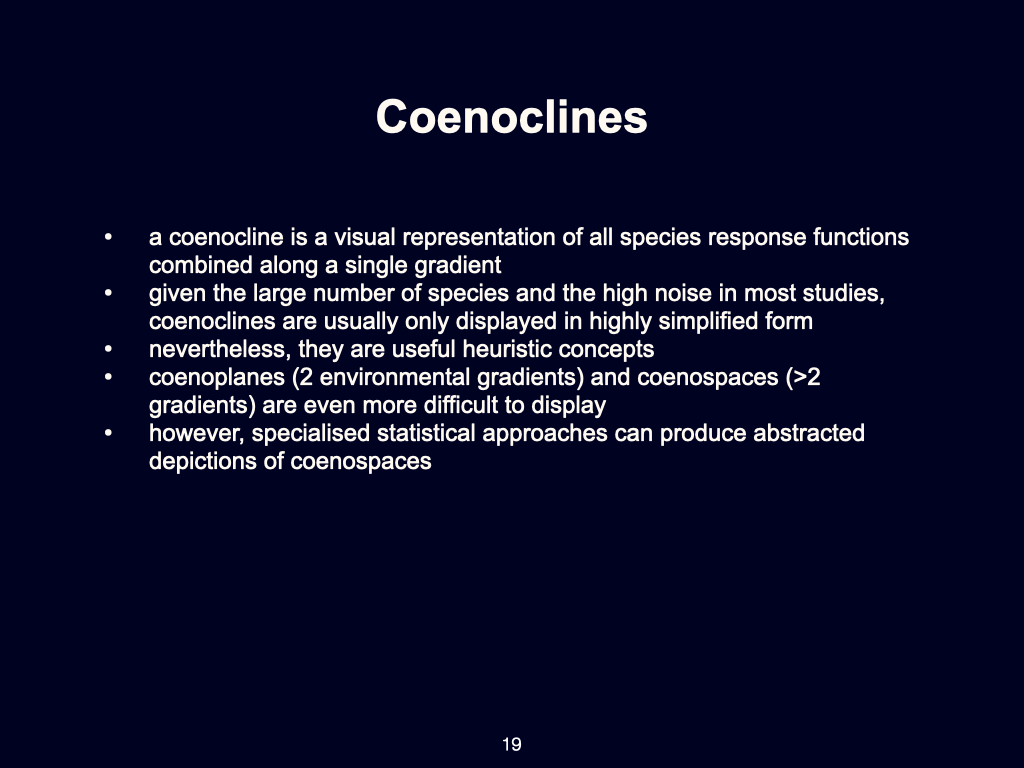
\includegraphics[width=0.8\linewidth]{../images/BDC334/BDC334-019.jpeg}
\caption*{Slide 19}
\end{figure}

\begin{figure}[ht]
\centering
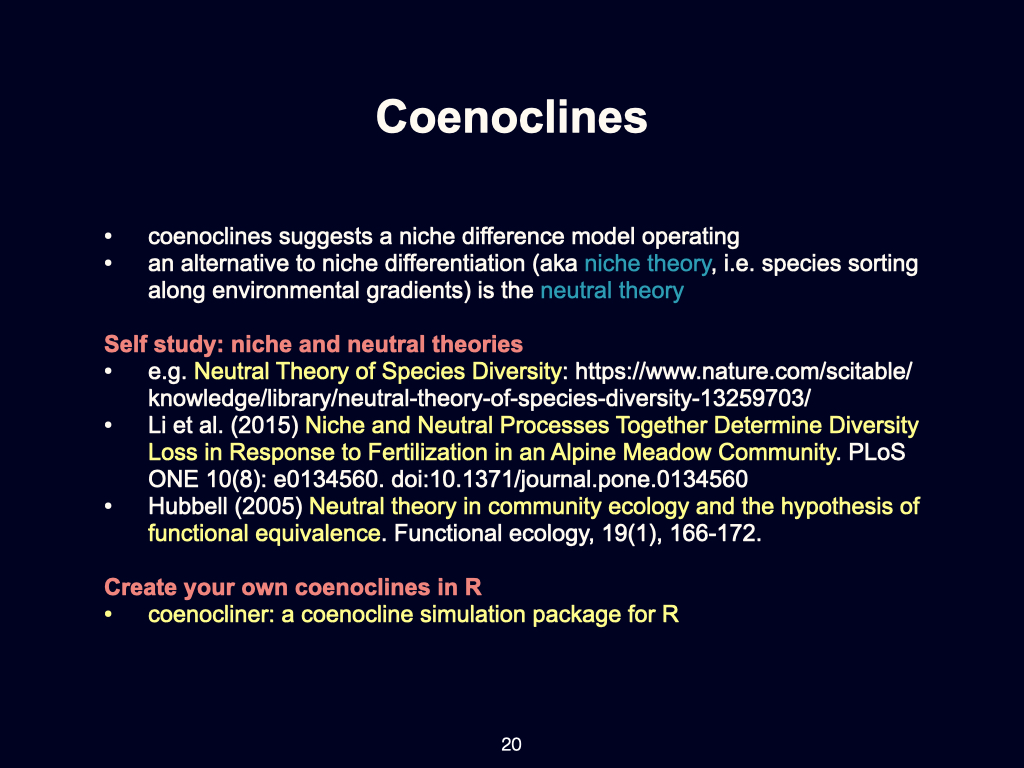
\includegraphics[width=0.8\linewidth]{../images/BDC334/BDC334-020.jpeg}
\caption*{Slide 20}
\end{figure}

A coenocline is essentially a more complex representation of species
distributions, where the response to every environmental variable and
every species on earth is superimposed to obtain a composite
visualisation (Slides 19-20). This is, as you can imagine, extremely
difficult to visualise directly, as it essentially combines all these
different gradients into one highly complex picture. A coenocline
represents the `sweet spot' or the shift in landscape associated with
changing environmental conditions and the location where particular
types of populations will peak in abundance.

Instead of just thinking of a gradient and a unimodal distribution for
one species, imagine a unimodal distribution for every species, across
every environmental condition that influences growth and fitness. When
you superimpose the outcomes, you produce what is called a coenocline.

If you examine two environmental dimensions together --- for example,
temperature and humidity --- this produces a two-dimensional plane
called a coenoplane. If you add additional variables, such as soil
characteristics, it becomes a multi-dimensional space called a
coenospace. A coenospace is, therefore, a multi-dimensional
representation of the best locations for collections of species given
all relevant environmental gradients.

This move from thinking about a single gradient to a complex coenocline
reflects a major step in understanding the ecology of species
distributions.

\section{Statistical Approaches}\label{statistical-approaches}

We have fairly specialised statistical methodologies for studying
coenoclines and related phenomena. We will touch briefly on some of
these in this module, though there may be challenges due to the need for
suitable computer lab access. Those of you progressing to honours will
take an entire module in Quantitative Ecology, which lasts six or seven
weeks and covers these statistical methods in greater depth ---
specifically targeting coenoclines, coenospaces, coenoplanes, and
associated analytical approaches.

\chapter*{Lecture 3c}\label{lecture-3c}
\addcontentsline{toc}{chapter}{Lecture 3c}

\section{The Earth System and Global
Change}\label{the-earth-system-and-global-change}

\begin{figure}[ht]
\centering
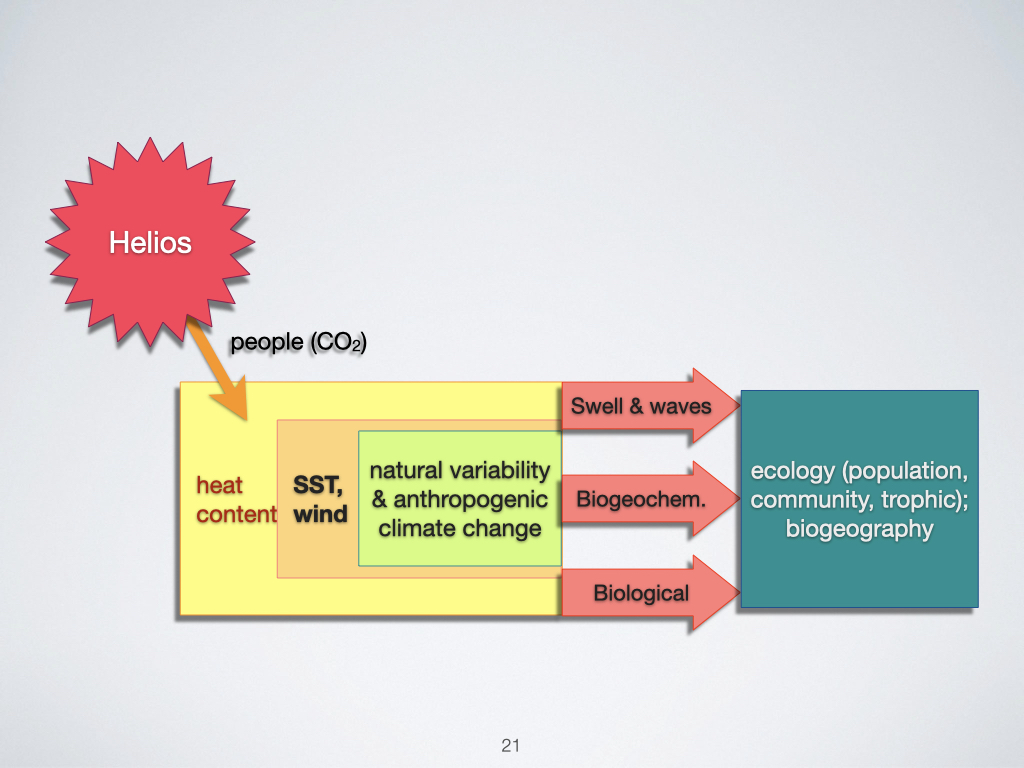
\includegraphics[width=0.8\linewidth]{../images/BDC334/BDC334-021.jpeg}
\caption*{Slide 21}
\end{figure}

Let us examine all the processes currently impacting Earth. In the age
we live in today, there is a particular need to be concerned with global
change, which encompasses a variety of components. The most obvious, and
certainly the most widely discussed in the popular media, is climate
change (Slide 21).

Climate change fundamentally arises due to the release of carbon dioxide
(\(\mathrm{CO}_2\)) into the atmosphere by human activity, particularly
through the burning of fossil fuels. This \(\mathrm{CO}_2\) does not
originate from the sun, but rather acts to trap the sun's energy within
our atmosphere, preventing it from escaping back into space. This
process leads to an accumulation of heat on Earth, which we observe as
an increase in the general heat content --- measured as a higher
temperature --- across the globe.

As more heat builds up, it causes changes in atmospheric pressure
systems. Regions warming up more than others develop areas of low
pressure, where air rises and circulates. As air rises, it contributes
to the formation of winds, and these changes in heat content are not
limited to the atmosphere alone. A significant proportion of this heat
is absorbed by the surface of the oceans, referred to as the sea surface
temperature (SST). As the ocean's surface absorbs this additional heat,
we see a rise in sea surface temperature.

\section{Atmospheric and Oceanic
Responses}\label{atmospheric-and-oceanic-responses}

One of the most measurable atmospheric responses to increased heat
content is an increase in global wind activity. Of course, the
real-world system is much more complex than this simple description, but
it provides a useful starting point. In the case of the ocean, the most
noticeable change is the rise in sea surface temperature. Both the
atmosphere and the oceans experience this rise in temperature, which
manifests as what we term anthropogenic climate change.

The implications of these temperature changes are profound. Many species
have evolved to thrive in relatively narrow environmental conditions ---
what we might refer to as ``sweet spots'' (not a technical term, so
don't use it when you communicate professionally). A particular plant,
for example, may be optimally adapted to the current temperature of Cape
Town. If Cape Town warms by \(2\,^\circ\mathrm{C}\), this plant finds
itself outside of its optimal range. At that point, it faces a choice:
it must either die out or, if its biological processes enable a
sufficiently rapid response, it can shift geographically to remain
within its preferred temperature range. This would require the plant to
``move'' towards the area where the climatic conditions mirror what used
to be present in Cape Town --- possibly to the west --- as the climate
envelope shifts.

So, climate change is already influencing the distribution of biota on
Earth. We must therefore be aware of climate change as a new, critical
process, and work to understand how it is likely to affect all aspects
of the environment --- particularly from both an ecophysiological and
ecological perspective. For marine systems, this includes not only
changes to swells and waves but also to the biogeochemistry of key
nutrients such as nitrogen, phosphorus, and carbon. Biological
interactions will change as well, exerting a profound influence on
population ecology, among other fields.

This means that all modern biologists must grapple with climate change
as an additional source of variation layered atop the myriad other
processes already operating within Earth's systems. Fully understanding
climate change --- and projecting its effects into the next \(100\) to
\(150\) years --- is critically important for anticipating how the
biogeography of the future world will differ from that of today.

\section{Regional Gradients: Focus on the
Ocean}\label{regional-gradients-focus-on-the-ocean}

\subsection{The Role of the Agulhas
Current}\label{the-role-of-the-agulhas-current}

\begin{figure}[ht]
\centering
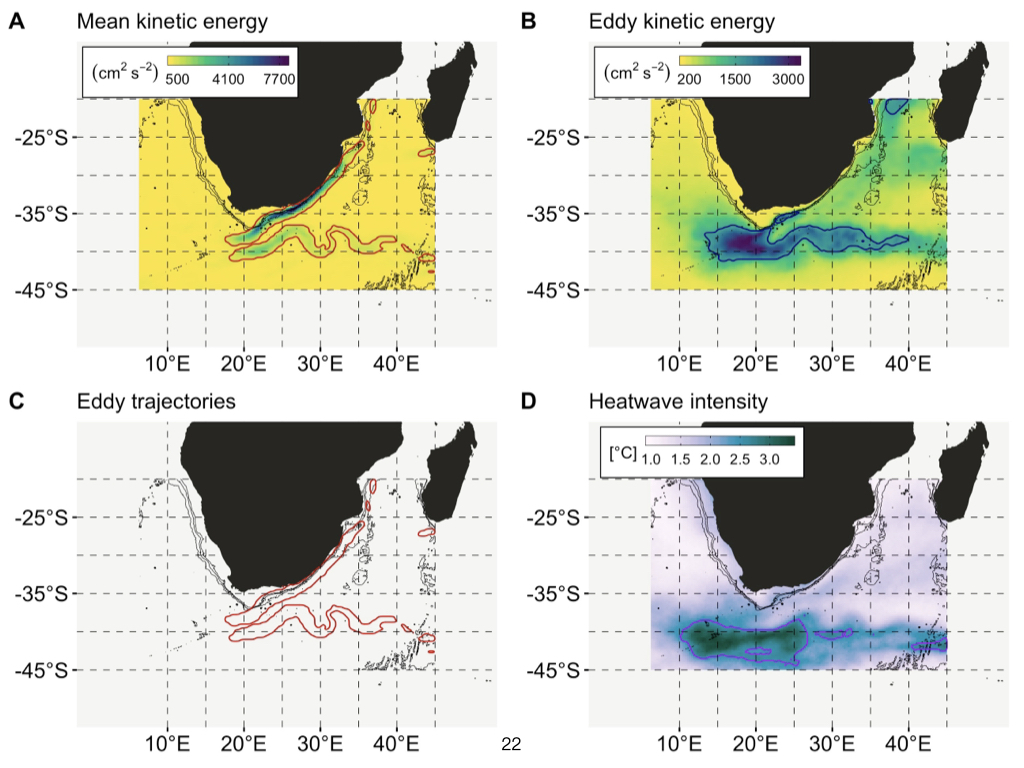
\includegraphics[width=0.8\linewidth]{../images/BDC334/BDC334-022.jpeg}
\caption*{Slide 22}
\end{figure}

Let me now focus more specifically on the ocean, as this is where much
of my research is conducted. One of the most influential systems
impacting South Africa --- as well as many other coastal regions
worldwide --- is the large ocean current running along our coast.
Although it appears snake-like on maps and diagrams, this is in fact the
Agulhas Current (Slide 22).

The Agulhas Current flows from the north, past South Africa's east
coast, moving southwards before looping back into the South Indian
Ocean. The water it transports from the north is warm, as it originates
close to the equator. Regions nearer the equator experience greater day
length and are closer to the sun, leading to higher heat absorption.
Therefore, both the ocean and the overlying atmosphere are warmer in
tropical regions.

This warm tropical water is carried southwards along the east coast of
South Africa, bringing it into regions that would otherwise be
significantly cooler. The presence of this warm water not only raises
the temperature of the overlying atmosphere, but also drives greater
rates of evaporation. As warm water evaporates, it injects moisture into
the atmosphere, which then becomes available for rainfall.

Within this system, the rising warm air over the ocean creates a
low-pressure area, while the relatively cooler land retains higher
pressure. This pressure differential drives winds from the ocean towards
the land, carrying with them moisture-laden air --- and, as a
consequence, there is considerable rainfall along South Africa's eastern
coastline.

If you recall the east-to-west rainfall gradient in South Africa ---
with KwaZulu-Natal in the east being particularly wet and moving towards
increasing aridity as you travel westward --- the Agulhas Current is
largely responsible. The abundance of moisture and rainfall along the
east coast owes much to the warmth of this current, which brings water
from the tropics and sustains the region's lush vegetation.

However, as you move away from the direct influence of the Agulhas
Current, further west towards central South Africa, the oceanic
influence diminishes. The water becomes colder, less moisture evaporates
from the surface, and significantly less rainfall occurs. This renders
the central and western regions of South Africa considerably drier and
more arid, with less vegetation and runoff.

\subsection{Western Boundary Currents around the
World}\label{western-boundary-currents-around-the-world}

This pattern is not unique to South Africa. Similar warm ocean currents
flow along the eastern margins of major continents and are collectively
known as western boundary currents. Examples include:

\begin{itemize}
\tightlist
\item
  The Brazil Current along the east coast of South America
\item
  The Gulf Stream along the east coast of North America
\item
  The Kuroshio Current off the east coast of Japan
\item
  The East Australian Current alongside eastern Australia
\end{itemize}

These currents, known as western boundary currents because they flow
along the western edge of their respective ocean basins, carry warm
water from the tropics into the mid-latitudes, depositing moisture-rich
air and promoting rainfall across large coastal regions.

As a general rule, continents influenced by these warm currents display
a moisture gradient from east to west. For example, in Brazil, the
region affected by the Brazil Current is warm and moist, but as one
travels westwards into the interior --- and especially into Chile and
Peru {[}attention: Chile and Peru are west of Brazil, but separated by
the Andes and not on the same cross-sectional gradient; this is an
oversimplification{]} --- the climate becomes progressively more arid.
Similar principles applies to North America and Australia.

\subsection{The Importance of Ocean Currents for Regional Climatic
Gradients}\label{the-importance-of-ocean-currents-for-regional-climatic-gradients}

Ocean currents play an absolutely critical role in establishing these
large-scale regional gradients, which then determine how vegetation and
associated biota are distributed. The moisture content of the
environment is the primary driver shaping these patterns, though other
factors become increasingly important as one moves further from the
influence of warm currents.

It is important to appreciate the significance of the Agulhas Current in
shaping South African climate and ecology. If you were to ``switch off''
the Agulhas Current and replace it with a cold current {[}attention: not
physically possible, but a useful thought experiment{]}, the entire east
of South Africa would resemble the arid, desert-like conditions
currently found along the west coast. Therefore, the ocean ---
specifically, these powerful currents --- is fundamental to the regional
climate patterns that support life as we know it on land.

If you wish to deepen your understanding, I suggest reading further
about the Agulhas Current and its effects. Its presence is precisely
what makes South Africa's eastern seaboard lush and habitable, in stark
contrast to the much drier west.

\chapter*{Lecture 3d}\label{lecture-3d}
\addcontentsline{toc}{chapter}{Lecture 3d}

\section{The Role of the Agulhas Current in Setting
Gradients}\label{the-role-of-the-agulhas-current-in-setting-gradients}

Another aspect that occurs due to the Agulhas Current is that, as the
current moves --- recall, as we travel from north to south, moving
progressively away from the tropical regions into the subtropics and
then into temperate regions --- evaporation happens along this journey.
The residual water in the ocean becomes increasingly cooler and cooler.
This cooling occurs because the heat that was originally in the ocean is
now being transferred into the atmosphere, warming the land adjacent to
it. Thus, as we head further south, the seawater temperature drops as
the heat from further north has dissipated and now resides in the
atmosphere and over the land.

\begin{figure}[ht]
\centering
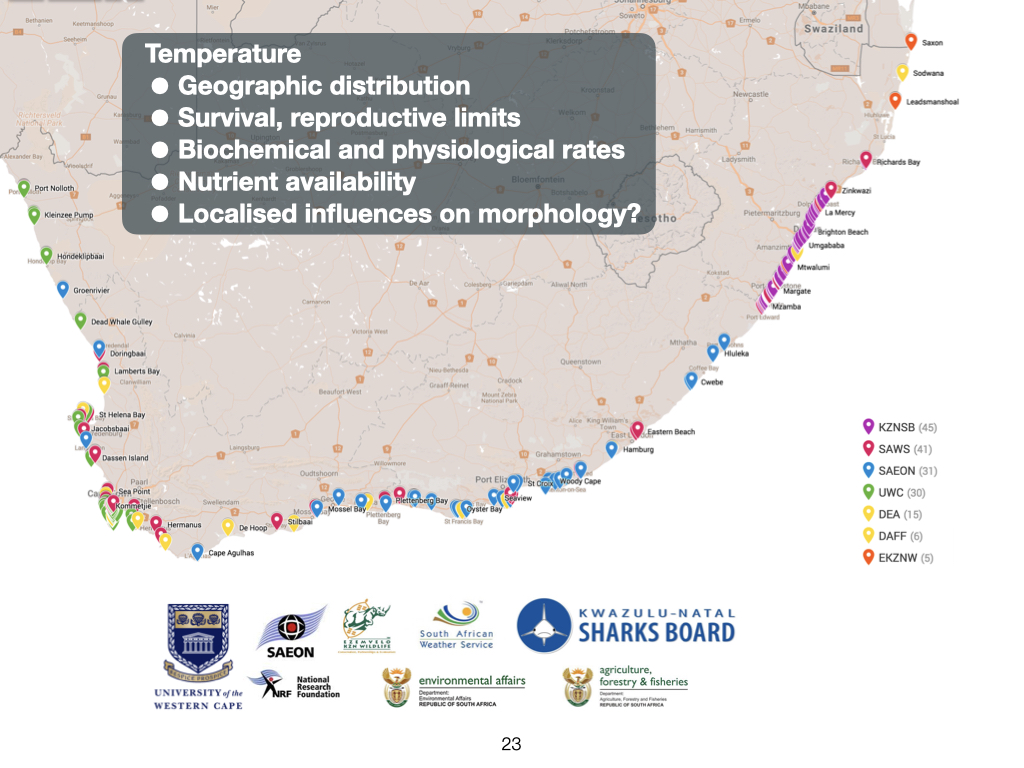
\includegraphics[width=0.8\linewidth]{../images/BDC334/BDC334-023.jpeg}
\caption*{Slide 23}
\end{figure}

Seawater in the southern regions is substantially colder compared to
somewhere like Durban (Slide 23). You can actually feel the difference.
By the time you reach Cape Town, the seawater is even colder, owing to
the presence of a different ocean current, which brings about a process
called upwelling rather than the warming effect of the Agulhas. So, in
addition to setting up a gradient over the land in terms of various
factors such as moisture, temperature, and erosion --- all processes
linked to rainfall --- the Agulhas Current also sets up a strong
temperature gradient along the coastline. At the northern border, north
of Sodwana Bay with Mozambique, sea temperatures are at their highest,
and as you progress down the coast, the temperature decreases
consistently, becoming coldest at Cape Town. Therefore, there is a
clear, almost linear, gradient in decreasing temperature from north to
south along the coast of South Africa. Again, this gradient is a direct
consequence of the Agulhas Current.

\section{Examples of Environmental Gradients in False
Bay}\label{examples-of-environmental-gradients-in-false-bay}

\begin{figure}[ht]
\centering
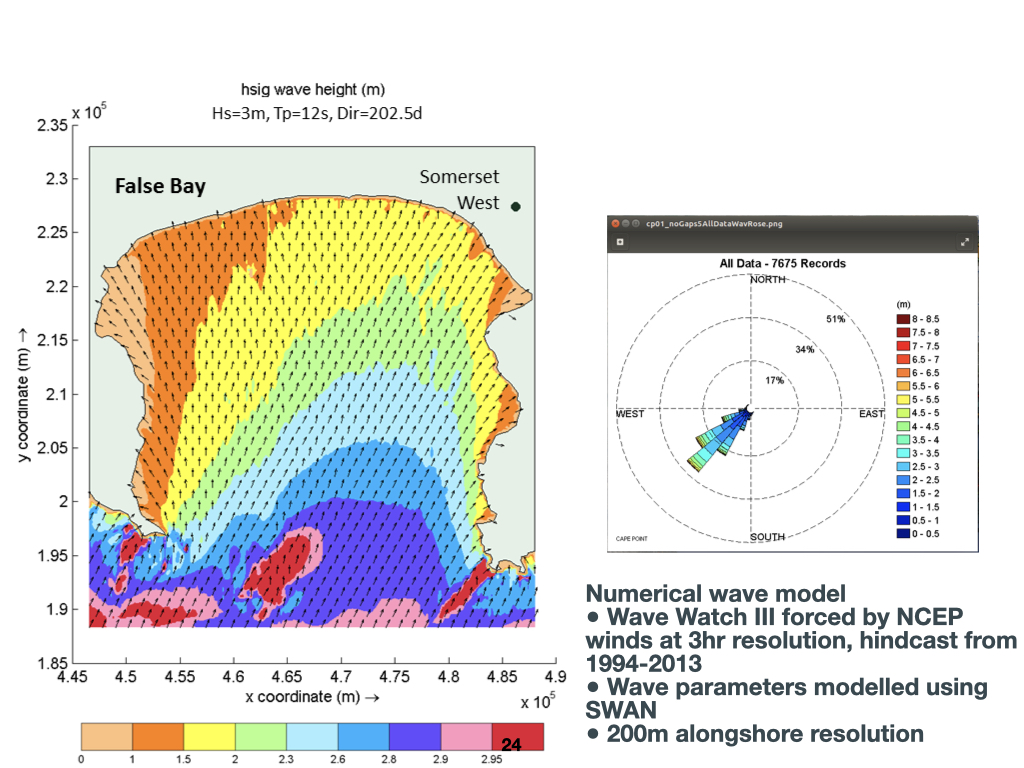
\includegraphics[width=0.8\linewidth]{../images/BDC334/BDC334-024.jpeg}
\caption*{Slide 24}
\end{figure}

Here is a figure illustrating waves --- this is False Bay (Slide 24).
This bay is where many of you find yourselves; Cape Town is in this
region. In the Southern Ocean, far south of South Africa, there are
strong prevailing winds that generate large swells, sometimes
originating \(1{,}000\)--\(2{,}000\) kilometres away. These waves
eventually propagate and arrive at the shores of False Bay as swells.

This is just one more example of a regionally important environmental
gradient. The spatial scale here is more restricted --- we are now
considering False Bay, which is about \(50\)--\(60\) kilometres across.
Even across such a small distance, you can observe a gradient: from the
sheltered western sides of False Bay, such as Muizenberg, which
experiences very low winds and small waves, moving south and east into
more exposed sections, the wave height increases substantially. Within
False Bay, there is a gradient in wave energy: lower in the west, higher
in the east, and peaking further south. On the other side of the Cape
Peninsula, exposed to the Atlantic, waves are higher still, as they
directly intercept swells from the South Atlantic Ocean.

Wave gradients, such as those found in False Bay, influence the
distribution of kelp and other marine organisms. Simultaneously, there
is a recognised temperature gradient across False Bay, as well as a
depth gradient: moving from the coastline towards central False Bay, the
water depth transitions from only \(1\)--\(3\) metres near the shore to
around \(70\) metres in the centre.

Remember from your BDC223 module: as we go deeper into the ocean, there
is a vertical light gradient --- the deeper you go, the less light is
available. Thus, environmental gradients exist at multiple dimensions:
horizontal gradients such as temperature, waves or salinity, and
vertical ones like light with depth.

\section{Gradients Across Scales: From Regional to
Global}\label{gradients-across-scales-from-regional-to-global}

These environmental gradients operate at multiple spatial scales ---
from gradients at the southern hemisphere or continental scale, to those
across a bay only a few dozen kilometres wide, right down to vertical
gradients in the ocean. On a planetary scale, gradients extend from the
tropics to the poles. All of these gradients, at every scale, are
responsible for allowing certain organisms to persist in particular
environments, while excluding others.

The work of ecologists, especially macroecologists, is to investigate
how these gradients structure the organisation of life across the
Earth's surface.

\section{Remote Sensing and Observing
Patterns}\label{remote-sensing-and-observing-patterns}

\begin{figure}[ht]
\centering
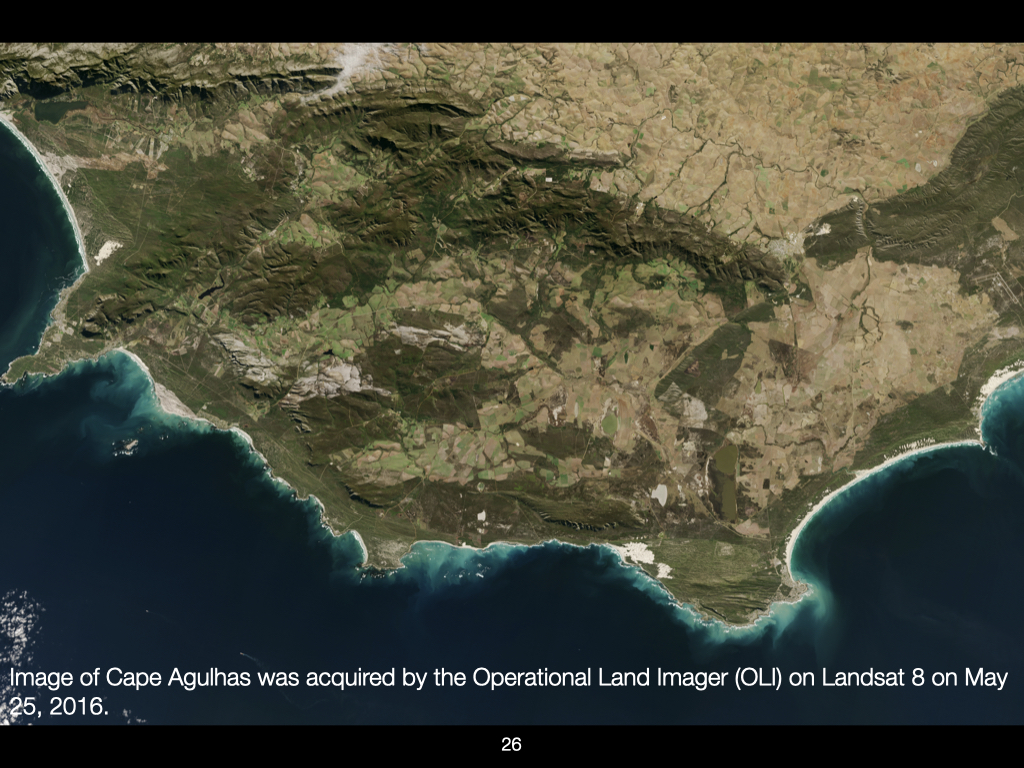
\includegraphics[width=0.8\linewidth]{../images/BDC334/BDC334-026.jpeg}
\caption*{Slide 26}
\end{figure}

Let us now look at an image of the Earth's surface. Ecology, in essence,
is the study of patterns. Here, you can observe a patchwork of different
colours --- dark green, brown, grey --- each representing distinct
surface properties or vegetation cover (Slide 26).

For instance, the regions with dark green typically indicate dense,
healthy vegetation --- vast patches of green associated with the Western
Cape. In other areas, browner patches mean the vegetation is more
scrubby, sparse, or replaced with barren sand.

Macroecologists would ask: why is this patch green and that patch brown,
sometimes only a few kilometres apart? Looking closely, greenness is
often associated with coastal zones, particularly along the Garden Route
and Western Cape. This is a function of atmospheric and oceanic
patterns, especially the influence of the Agulhas Current. However, in
some regions, especially inland, apparent greenness in satellite images
may be attributable to intensive farming and land transformation, rather
than natural processes. {[}attention: Not every green patch is natural
vegetation; some are vineyards, canola, or other agricultural fields.{]}

If you zoom in, you can see a clear patchwork reflective of agricultural
practices such as viticulture and other crops. Remaining tracts of
natural fynbos are also visible, structured according to elevation: lush
and green in valleys, but sparse and grey at higher altitudes ---
demonstrating how temperature and exposure control plant community
composition even at relatively small spatial scales.

\section{Using Temporal Data to Track Environmental
Change}\label{using-temporal-data-to-track-environmental-change}

Satellite data have been available daily since 1981. Comparing
present-day maps to those from one decade ago, or two decades ago,
reveals changes in landscape patterns. These shifts are mostly
consequences of anthropogenic environmental modification: farming,
deforestation, urbanisation, and fire. In some places, you can also
observe temporary or seasonal phenomena like snow cover.

\section{Integrating Multiple Types of Environmental
Information}\label{integrating-multiple-types-of-environmental-information}

From a single remote sensing image, you can extract vast quantities of
information --- vegetation type, land use, altitude and topography,
river catchments, coastal processes, and more. For example, wave action
stirs up sand in the water, which appears milky blue or white from
space, especially where long sandy beaches are present. Rocky areas have
less suspended sediment, and thus appear darker in satellite imagery.
Visible drainage lines indicate the position of rivers and the amount of
water they transport.

At even finer scales, satellite imagery can be used to monitor fire
scars and the impact of wildfire, as fires appear starkly in the
imagery.

\section{Biological Productivity and the Agulhas
Bank}\label{biological-productivity-and-the-agulhas-bank}

\begin{figure}[ht]
\centering
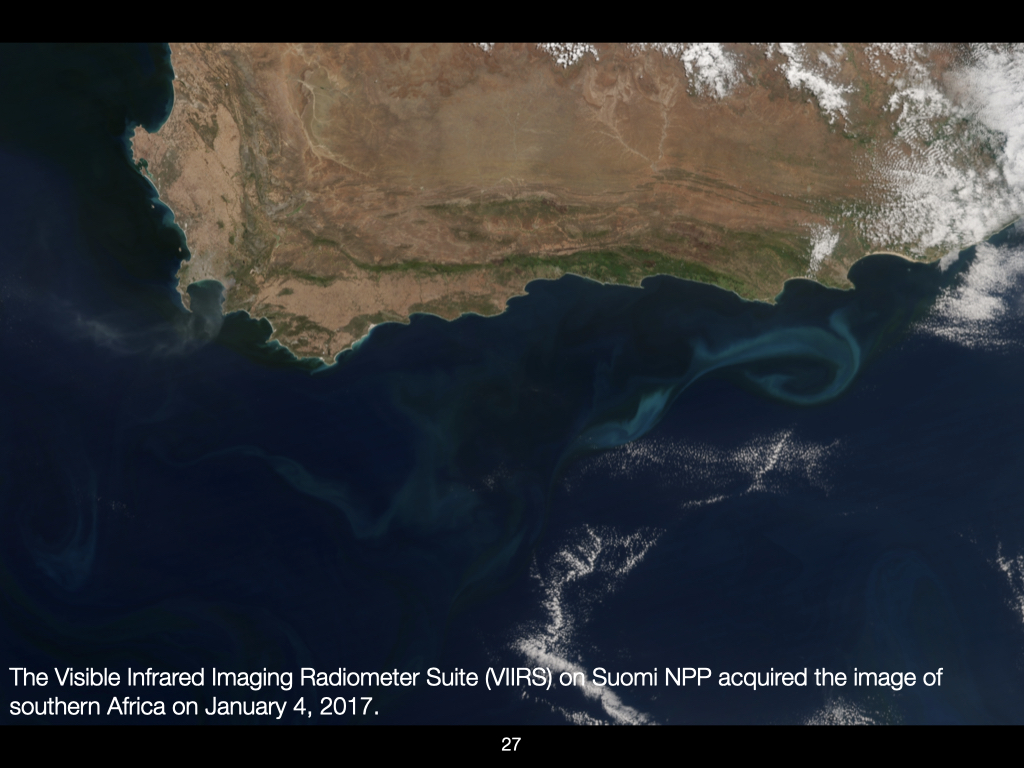
\includegraphics[width=0.8\linewidth]{../images/BDC334/BDC334-027.jpeg}
\caption*{Slide 27}
\end{figure}

Here's another satellite image of South Africa. Again, there's False
Bay, and some white regions here are clouds, but look at these pale blue
swirls in the ocean --- these are areas of phytoplankton bloom.
Interestingly, these blooms are restricted in location due to the
dynamics of the Agulhas Current. Phytoplankton that drift into the
Agulhas Current quickly get swept away, so their retention above the
Agulhas Bank (Slide 27) --- a region extending up to \(200\) kilometres
offshore but with a maximum depth of about \(150\) metres --- is
especially significant for local productivity.

\section{Infrared Imagery and Vegetation
Detection}\label{infrared-imagery-and-vegetation-detection}

\begin{figure}[ht]
\centering
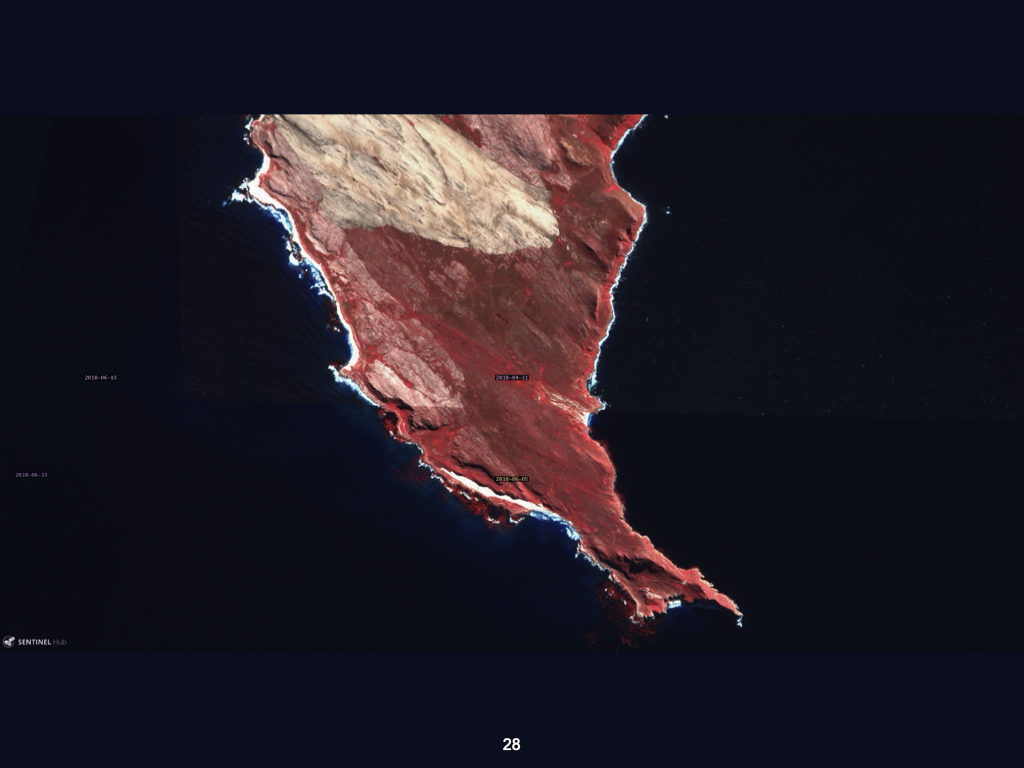
\includegraphics[width=0.8\linewidth]{../images/BDC334/BDC334-028.jpeg}
\caption*{Slide 28}
\end{figure}

Here, in an infrared image of the tip of the Cape Peninsula (Slide 28),
you can clearly distinguish natural vegetation, which appears in red,
from exposed bedrock and sand, which appear white. Off the coast, red
patches indicate the presence of kelp beds and kelp forests, which are
so large and dense they can be detected from space.

\section{The Macroecologist's
Challenge}\label{the-macroecologists-challenge}

All of this information --- vegetation types, land use, altitudinal
patterns, wave exposure, kelp forests, riverine systems, and even the
presence of fire --- can now be accessed and analysed by
macroecologists. Our task in this module is to understand how to use
such data, and thereby to interpret how the physical environment
structures patterns of life at a range of scales.

\section{Assignment Instructions}\label{assignment-instructions}

\begin{figure}[ht]
\centering
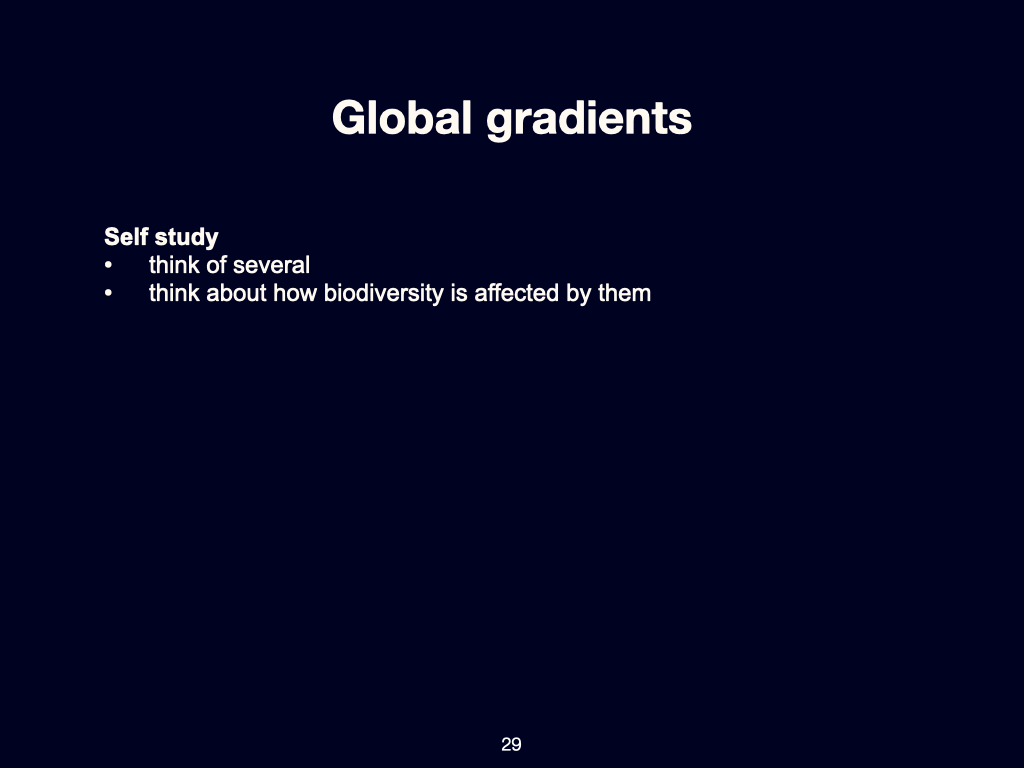
\includegraphics[width=0.8\linewidth]{../images/BDC334/BDC334-029.jpeg}
\caption*{Slide 29}
\end{figure}

To conclude, as a preparation for an upcoming assignment, I would like
you to select two or three examples of environmental gradients you can
identify --- some operating at local, others at regional, and others at
global scales (Slide 29). Prepare an essay, according to the specific
guidelines I'll provide shortly, in which you explain in detail how
these gradients are capable of structuring biodiversity.

\chapter{Biodiversity Concepts}\label{biodiversity-concepts}

\begin{tcolorbox}[enhanced jigsaw, colback=white, bottomrule=.15mm, opacitybacktitle=0.6, arc=.35mm, opacityback=0, left=2mm, coltitle=black, colframe=quarto-callout-note-color-frame, breakable, bottomtitle=1mm, toptitle=1mm, toprule=.15mm, titlerule=0mm, leftrule=.75mm, title=\textcolor{quarto-callout-note-color}{\faInfo}\hspace{0.5em}{BCB743}, colbacktitle=quarto-callout-note-color!10!white, rightrule=.15mm]

This material must be reviewed by BCB743 students in Week 1 of
Quantitative Ecology.

\end{tcolorbox}

\begin{tcolorbox}[enhanced jigsaw, colback=white, bottomrule=.15mm, opacitybacktitle=0.6, arc=.35mm, opacityback=0, left=2mm, coltitle=black, colframe=quarto-callout-note-color-frame, breakable, bottomtitle=1mm, toptitle=1mm, toprule=.15mm, titlerule=0mm, leftrule=.75mm, title=\textcolor{quarto-callout-note-color}{\faInfo}\hspace{0.5em}{Also see:}, colbacktitle=quarto-callout-note-color!10!white, rightrule=.15mm]

It is important that you accompany your reading of this chapter with the
material presented in \href{Lab-03-biodiversity.html}{Lab 3} and the
online content on \href{Lec-04-biodiversity.html}{Tangled Bank}.

\end{tcolorbox}

\chapter*{Lecture 4a}\label{lecture-4a}
\addcontentsline{toc}{chapter}{Lecture 4a}

\section{Introduction to
Biodiversity}\label{introduction-to-biodiversity}

Today, we'll be discussing the various concepts of biodiversity. This
concerns how we quantify diversity, both in terms of which species are
present and the proportions of those species existing within a
particular habitat, environment, or ecosystem. The key concepts to focus
on include alpha, beta, and gamma diversity --- those are the three
Greek-lettered types.

At its most basic, we use what are called univariate measures. That is,
all the variety of plants, animals, and things that are neither plant
nor animal can be condensed into a single measurement --- one variable.
That's essentially what ``univariate'' means: one variable.

\section{Univariate Indices and
Overview}\label{univariate-indices-and-overview}

To make this clearer, let's consider the UWC Nature Reserve --- you know
where it is. It contains a wide array of plants and animals, but all of
that complexity can be reduced to a single measurement for alpha, beta,
or gamma diversity.

Focusing specifically on alpha and gamma diversity, the univariate
measurements commonly used are the Shannon and Simpson indices. These
are the two most typical ways you'll see alpha and gamma diversity
quantified, and I'll give more detail shortly on what those indices are
and how they're applied.

\section{Alpha Diversity}\label{alpha-diversity}

\subsection{What is Alpha Diversity?}\label{what-is-alpha-diversity}

\begin{figure}[ht]
\centering
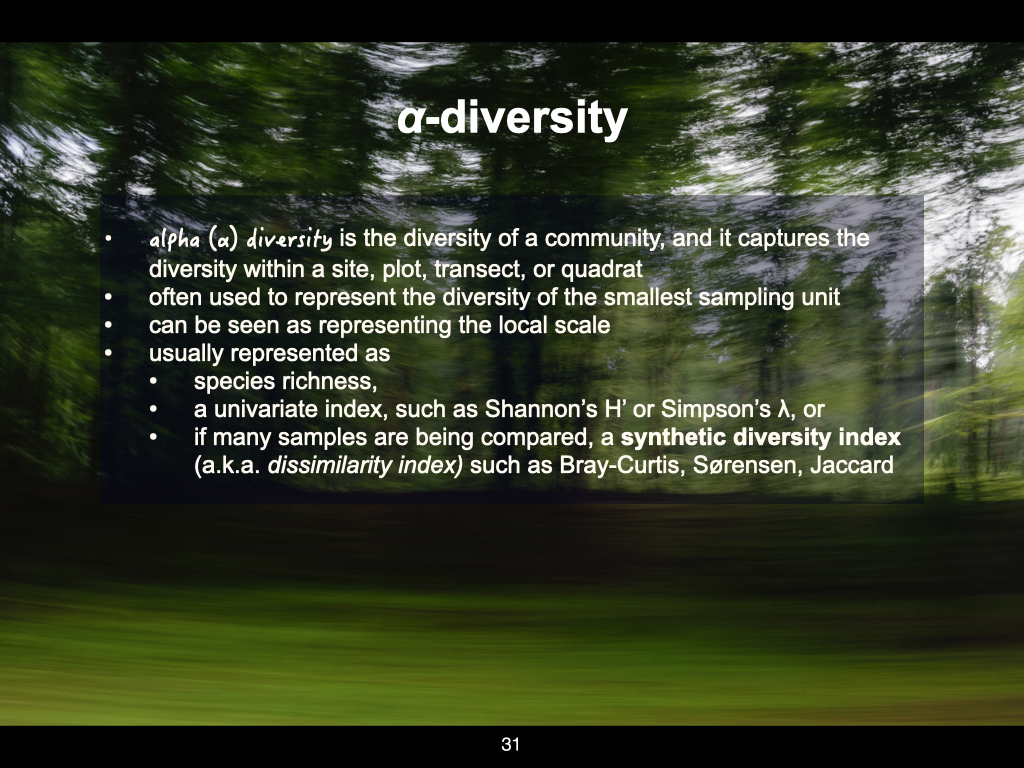
\includegraphics[width=0.8\linewidth]{../images/BDC334/BDC334-031.jpeg}
\caption*{Slide 31}
\end{figure}

Let's look first in more detail at alpha diversity (Slide 31). Alpha
diversity is the diversity of a community, plot, habitat, or ecosystem
at the smallest scale at which we measure. Returning to the UWC Nature
Reserve example, if we wish to know what plants and animals are present,
the standard approach in ecology is to lay down various transects or
plots --- also called quadrats --- across the area.

Quadrats are simply small subsections or representations, essentially
samples, of a much larger environment. We use a sufficiently large
number of quadrats to try to capture the full range of biodiversity in a
given place. Alpha diversity, therefore, accounts for diversity at this
very local, smallest scale.

\subsection{How Do We Measure Alpha
Diversity?}\label{how-do-we-measure-alpha-diversity}

For example, if you place a single quadrat within the entire UWC Nature
Reserve, that quadrat forms the basis for measuring or representing
alpha diversity. Alpha diversity is essentially biodiversity at the
local scale, and there are three principal ways to express it:

\begin{enumerate}
\def\labelenumi{\arabic{enumi}.}
\item
  \textbf{Species Richness:}\\
  The simplest measure is just counting the number of species present.
  For example, ``There are \(15\) species of plants and \(12\) species
  of vertebrates'' within the UWC Nature Reserve. At the smallest scale,
  this involves counting the number of plant and animal species within a
  single quadrat.
\item
  \textbf{Indices (Shannon and Simpson's):}\\
  You can also use indices, such as the Shannon or Simpson index. These
  take into account not only the number of species (species richness)
  but also the abundance or ``how much'' of each species is present in
  your quadrat.
\item
  \textbf{Dissimilarity Indices:}\\
  A more complex way involves looking at all the quadrats placed within
  an area at once, quantifying differences between them. While species
  richness or the univariate indices often focus on the individual
  quadrat, you can compare every quadrat pairwise with every other to
  create a dissimilarity index. Common dissimilarity indices include
  Bray--Curtis similarity, Sørensen dissimilarity, and Jaccard
  dissimilarity.
\end{enumerate}

Bear in mind, I'll touch more on dissimilarity indices in another
lecture. But for now, recognise that the synthetic diversity indices
mean comparing every quadrat with every other, using a variety of
metrics. Besides Bray--Curtis, Sørensen, or Jaccard, there are at least
another \(21\) such metrics or more.

\subsection{Interpreting Diversity
Metrics}\label{interpreting-diversity-metrics}

It's rather like measuring distance with a ruler. The ruler might be
marked in centimetres, and in the same way, indices such as
Bray--Curtis, Sørensen, Simpson, or Shannon are the ``rulers'' you use
for biodiversity. The actual value you get is measured in units of that
respective index, indicating biodiversity in quantifiable terms.

\section{Beta Diversity}\label{beta-diversity}

\begin{figure}[ht]
\centering
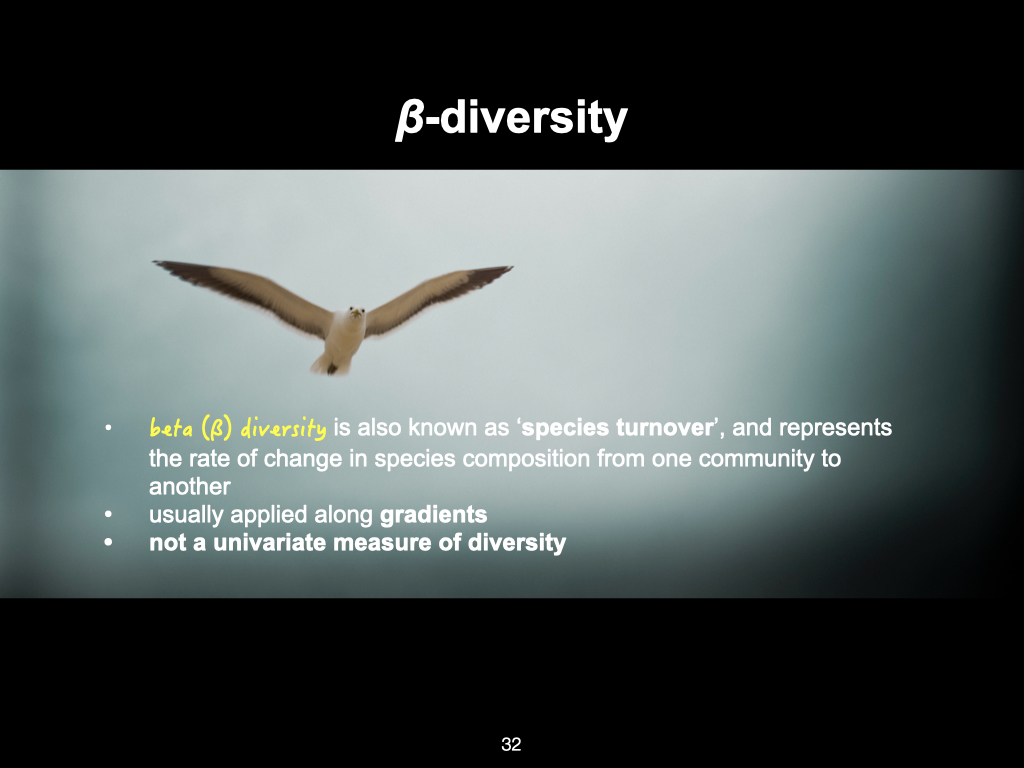
\includegraphics[width=0.8\linewidth]{../images/BDC334/BDC334-032.jpeg}
\caption*{Slide 32}
\end{figure}

\subsection{What is Beta Diversity?}\label{what-is-beta-diversity}

Beta diversity, by contrast, is sometimes referred to as ``species
turnover.'' It measures how different each quadrat placed within a
habitat is from every other quadrat --- essentially, the variation from
place to place across the landscape (Slide 32). In this way, it
quantifies heterogeneity --- how communities differ from spot to spot.

\subsection{Beta Diversity Along
Gradients}\label{beta-diversity-along-gradients}

To make this real, recall the example from last week: the temperature
gradient along the east coast of South Africa. As you move from Sodwana
Bay southwards, the temperature changes gradually. The further you go,
the more the temperature differs from your starting point. As this
physical variable changes, so too does the potential for different types
of plants and animals to exist. Thus, species composition shifts along
the gradient.

Beta diversity works particularly well in these scenarios, where we
measure community structure along environmental gradients. There is a
paper I've uploaded to Econva (and another associated one), which
provides visual explanations for how environmental gradients influence
beta diversity. Please make sure to look at those.

\subsection{Summary on Beta Diversity}\label{summary-on-beta-diversity}

Beta diversity is the second major measurement of biodiversity, highly
useful for examining how quickly communities change along gradients. As
the environment changes --- temperature, rainfall, soil type, etc. ---
so too does the composition of plants and animals, and beta diversity
allows us to quantify that change across the landscape.

\chapter*{Lecture 4b}\label{lecture-4b}
\addcontentsline{toc}{chapter}{Lecture 4b}

\section{Gamma Diversity: The Largest
Scale}\label{gamma-diversity-the-largest-scale}

\begin{figure}[ht]
\centering
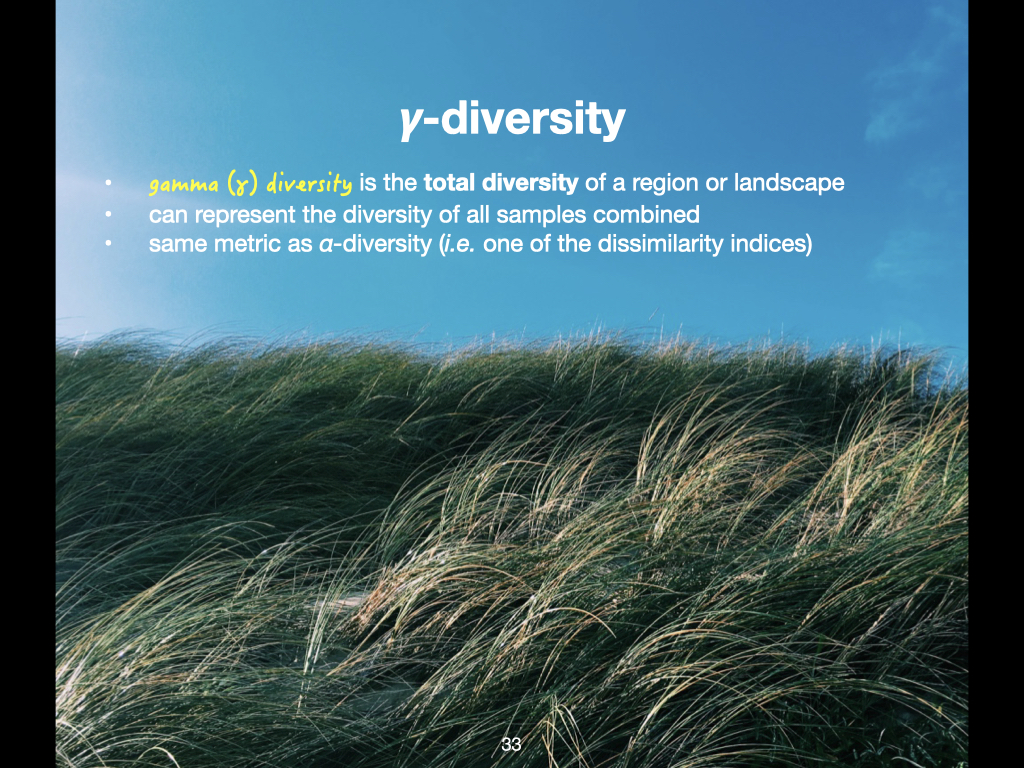
\includegraphics[width=0.8\linewidth]{../images/BDC334/BDC334-033.jpeg}
\caption*{Slide 33}
\end{figure}

At the very largest scale, the total amount of biodiversity is generally
called gamma diversity (Slide 33). If we go back to our example of the
UWC Nature Reserve, let us say we place one quadrat, and within that
single quadrat, we find seven species of plants and two species of
vertebrates. The total diversity for that quadrat would then be seven.

However, if we place multiple quadrats throughout the UWC Nature
Reserve, with each new quadrat, we are likely to encounter new species.
The more quadrats we place, the more species we will count, because
species are distributed across the landscape. Thus, gamma diversity
examines the diversity of the entire UWC Nature Reserve, and states that
there are, for example, 23 species of plants and seven species of
vertebrates across the whole reserve.

Gamma diversity can also be considered at even greater scales. It can
scale up to the entire planet, to all of Earth, at which point we might
say that the Earth has \(X\) million species of organisms. So, the
entire Earth represents the largest possible scale at which we can
account for the total number of living organisms, or species of living
organisms, present on the planet.

\section{Local and Regional Scales}\label{local-and-regional-scales}

At smaller scales, a continent could be considered a sampling unit. As
an example, Africa might have \(X\) hundred thousand species of
organisms, and South America another \(X\) hundred thousand, depending
on definitions and available data. In this context, the ``local'' scale
could be a country, so if we look at species within South Africa, for
example, that could be defined as alpha diversity.

Alpha diversity and gamma diversity are both measures that can, in
principle, apply to a very localised area. The largest possible extent
of that localised environment, such as the outer boundaries of the UWC
Nature Reserve, would count as gamma diversity for that smaller study.
If the study is instead concerned with the whole planet, then the entire
Earth is gamma diversity, and the continent, country, or region becomes
the scale for measuring alpha diversity.

\section{Defining the Scales: Researcher's
Perspective}\label{defining-the-scales-researchers-perspective}

Whether we use alpha or gamma diversity depends very much on the
research question. These terms are not fixed; as an investigator, it is
up to you to define the minimum and maximum extents of your study. For
example, if you are interested in the flora of the Western Cape, you
would draw a boundary around the Western Cape and define your gamma
diversity as all the species observed within those boundaries.

For alpha diversity in this context, you might look at the number of
species present in Belleville, in Rondebosch, in Worcester, and so forth
--- each a different locality within your region of study. Hence, the
use of alpha and gamma diversity depends entirely upon your definition
and the scale at which your research is taking place. The concept is
flexible, and is relative to the extent of your particular study ---
what is ``gamma diversity'' for one study may be ``alpha diversity'' for
a larger study, and so forth.

\section{Species Richness}\label{species-richness}

\begin{figure}[ht]
\centering
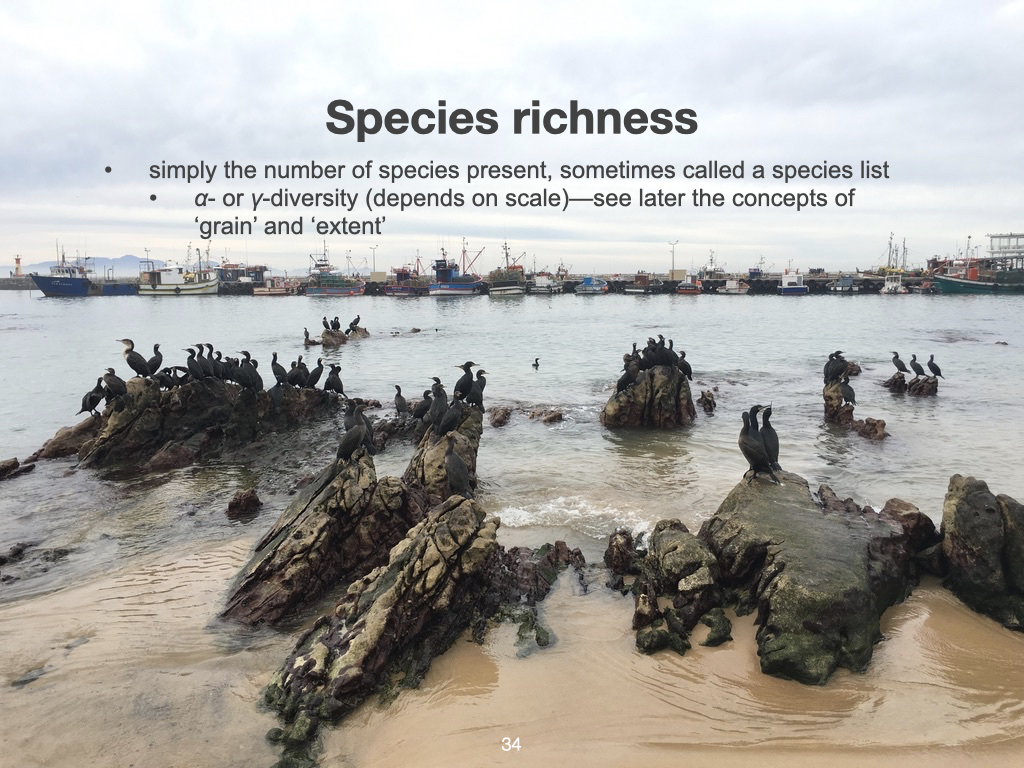
\includegraphics[width=0.8\linewidth]{../images/BDC334/BDC334-034.jpeg}
\caption*{Slide 34}
\end{figure}

Species richness is a term that brings us back to both alpha and gamma
diversity (Slide 34). As I have mentioned before, species richness is
simply the number of different species present. Measured at a small,
highly localised scale, species richness gives alpha diversity. Measured
across the full extent of your study region, species richness provides
gamma diversity. Both are ultimately just a count of how many species
are present.

\begin{figure}[ht]
\centering
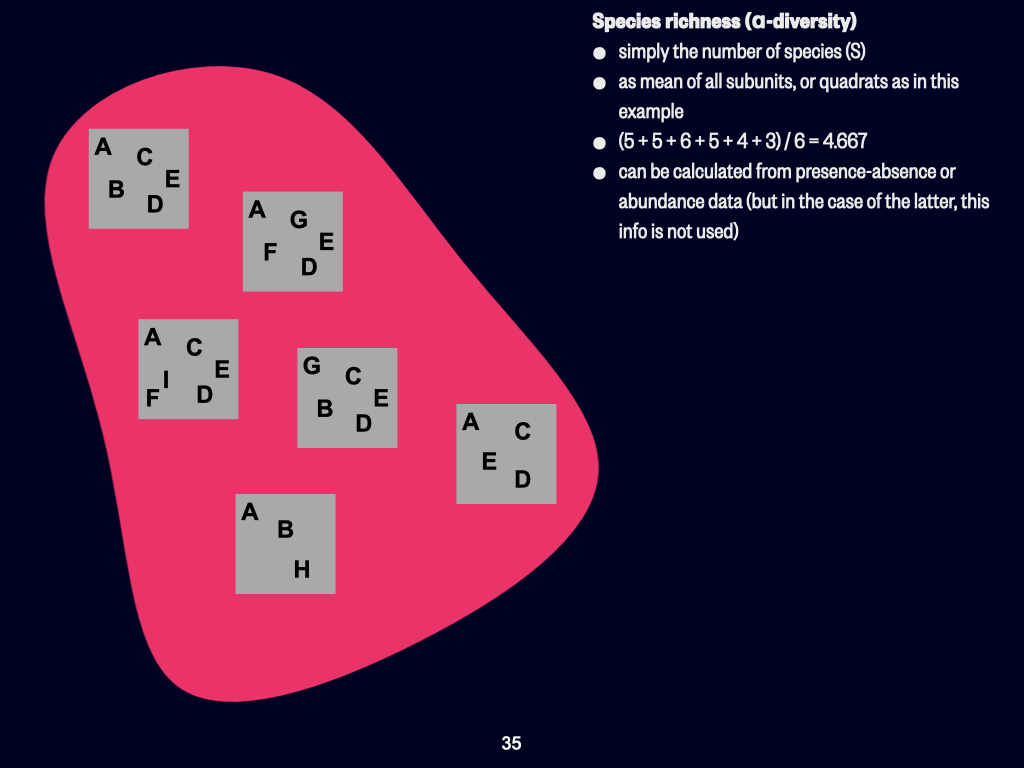
\includegraphics[width=0.8\linewidth]{../images/BDC334/BDC334-035.jpeg}
\caption*{Slide 35}
\end{figure}

Imagine a pink area, representing your total study habitat --- this is
your study area (Slide 35). You cannot count every single organism
within this space, so you sample by placing quadrats (the grey squares),
each representing a subset of the biodiversity present. If you deploy
enough quadrats, your sampling will hopefully capture every species
present in your study area.

For each quadrat, you tally up the number of different species present.
For example, one quadrat might contain five species. Another might
contain three. Some quadrats share species, others have unique species.
Suppose you have six quadrats, and their species richness values are
\(5\), \(5\), \(6\), \(5\), \(4\), and \(3\). To calculate the average
species richness for the landscape, you simply find the mean:

\[
\frac{5 + 5 + 6 + 5 + 4 + 3}{6} = 4.667
\]

\begin{figure}[ht]
\centering
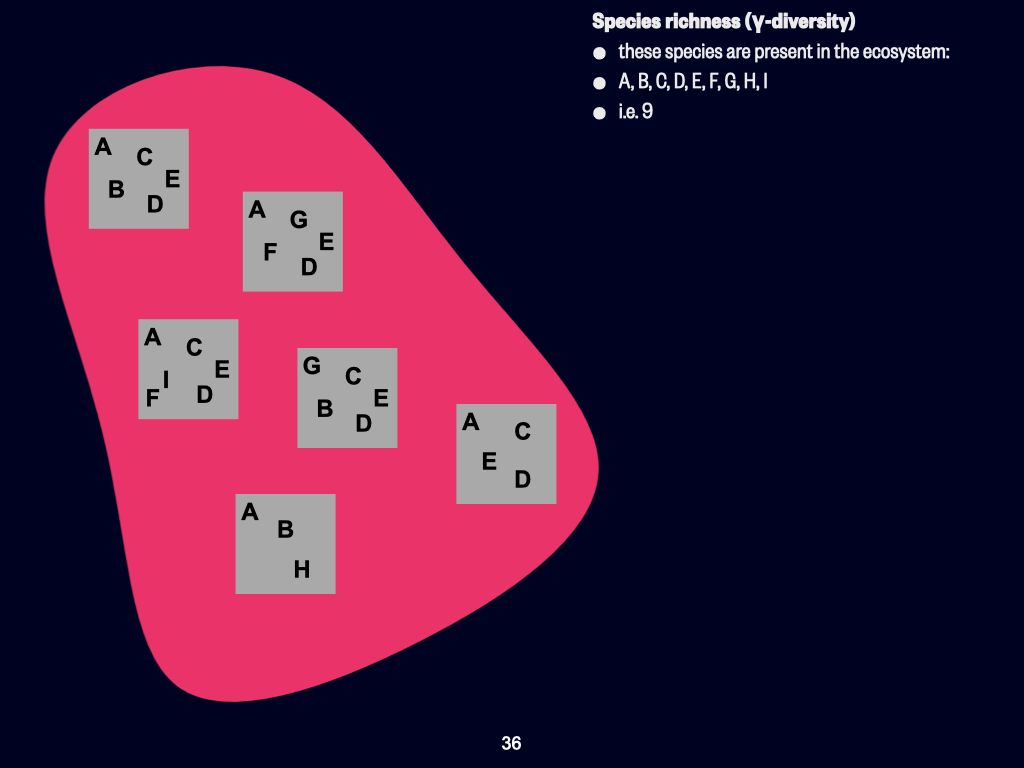
\includegraphics[width=0.8\linewidth]{../images/BDC334/BDC334-036.jpeg}
\caption*{Slide 36}
\end{figure}

This is your average species richness. At the largest scale, you simply
count the unique species present across all quadrats. If, collectively,
across all quadrats, there are nine unique species, then the gamma
diversity for that region is \(9\) (Slide 36).

\section{Beta Diversity: Measuring
Variation}\label{beta-diversity-measuring-variation}

\begin{figure}[ht]
\centering
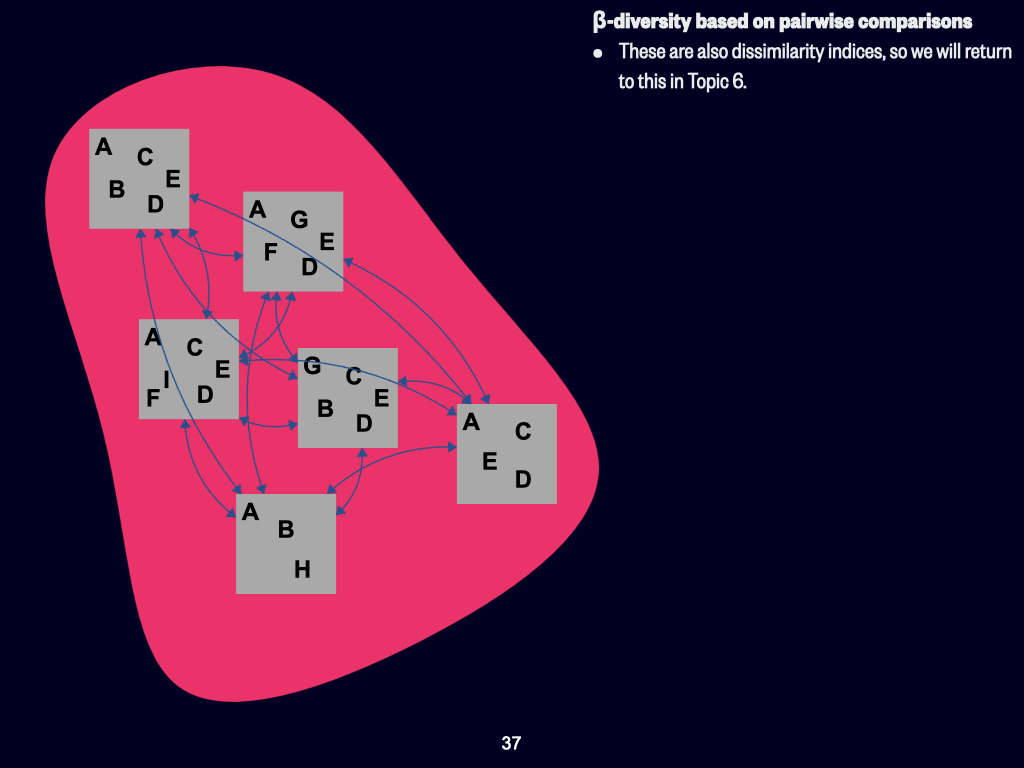
\includegraphics[width=0.8\linewidth]{../images/BDC334/BDC334-037.jpeg}
\caption*{Slide 37}
\end{figure}

Now let us move to beta diversity (Slide 37). Beta diversity focuses on
how different each quadrat is from every other quadrat; it measures
turnover in species composition. For instance, if one quadrat contains
species A, D, B, C, and E, and the quadrat next to it contains A, D, F,
G, and E, you see that they share two species (A and D), but differ by
three species each. Similarly, quadrats below or adjacent to one another
can be compared in the same way.

To calculate beta diversity, you must compare every quadrat to every
other quadrat --- that is, for every possible pair of quadrats, you
calculate the number of shared and unique species. This results in a
table of dissimilarity values (a dissimilarity index), where each value
shows how different one quadrat is from another.

We will discuss dissimilarity indices and how to interpret them in
detail in a later section of the course, where I shall provide some
pre-calculated examples for you to practise with.

The important point is that the landscape is almost never perfectly
homogeneous. For example, perhaps most quadrats have species A (present
in five quadrats) but not all. Species B might be present in three
quadrats, not everywhere else, and so on. In general, almost every
quadrat will be at least slightly different from the next. Beta
diversity captures the amount of this variation, or heterogeneity, in
your study landscape.

\begin{figure}[ht]
\centering
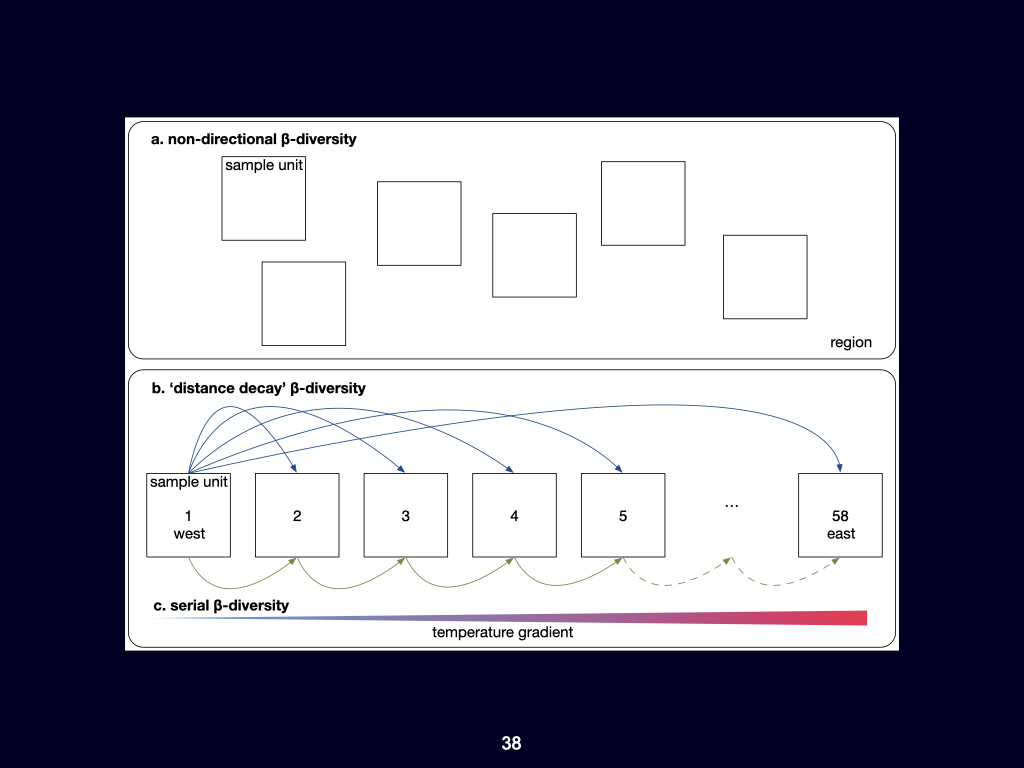
\includegraphics[width=0.8\linewidth]{../images/BDC334/BDC334-038.jpeg}
\caption*{Slide 38}
\end{figure}

Okay, continuing with our example of beta diversity, there are two
different ways in which we can approach beta diversity (Slide 38). One
is, as shown in the top panel --- Slide 38 (a) --- we assume that there
is no spatial relationship between one sampling unit and the next. So,
they are unordered across the landscape. This is the typical inference
we can make about biodiversity: we compare every unit to every other
unit. This is similar to the previous illustration in the earlier slide
we saw.

However, if we take a more structured approach to how we measure beta
diversity across the landscape --- looking at the bottom panel, panels
(b) and (c) --- we see that the sampling units are arranged in a logical
order. In this example, they are spatially arranged in increasing
distance from the west of the country.

This is the example of the seaweed data in Smit et al.~(2017): site
number one (sampling unit one) is in the west, and we move all the way
to sampling unit number 58, which is situated far to the east.

Now, if we take one sampling unit --- for instance, sampling unit number
one in the west --- and use that as the reference unit (it remains
constant, fixed in the west), we can then compare it to sampling unit
number two, next to it. We'll see that the difference in biodiversity
between one and two is going to be quite slight, because the spatial
distance between those two units is only about \(50\mathrm{km}\) or so.

If we compare sampling unit number three to sampling unit number one,
the spatial distance increases to about \(100;\mathrm{km}\), so there's
a slight increase in the beta diversity between those two pairs of
sites. Next, we compare site number five, which is about
\(200;\mathrm{km}\) further to the east, to site number one. In this
case, the change in dissimilarity between one and five is a bit greater.

So, the larger the distance becomes between a pair of sites, the greater
the change in the underlying environmental variables due to the
environmental gradient along the coast. Consequently, the species
dissimilarity also increases. The greater the distance between a pair of
sites, the more dissimilar they become.

By the time we reach section number 58, far to the east, the distance
between sites one and 58 is about \(2{,}700\) to
\(2{,}800 \mathrm{km}\). The environmental conditions in the subtropical
northeastern part of South Africa are very different from the cold
temperate conditions in the western part of the country. Consequently,
the species diversity is also vastly different. Virtually no species are
in common between sites one and 58. In contrast, when comparing sections
one and two, or sections one and three, because they are closer
together, the environments are more similar, and more species will be in
common.

This approach, which I've just explained, is called distance-decay beta
diversity.

Serial beta diversity takes another approach --- shown in portion (c) of
the figure. In this approach, we compare section one with section two:
the difference in beta diversity is slight. Then section two to section
three --- again, a slight difference. Section three to section four ---
still very small.

If we take the cumulative dissimilarities between every consecutive pair
of sites in the sequence from west to east, we find that the overall
beta diversity is the same as the difference between site one and site
58. So, the sum of consecutive pairwise comparisons adds up
(more-or-less) to the total beta diversity measured across the entire
distance between sites one and 58.

\section{Heterogeneity and
Homogeneity}\label{heterogeneity-and-homogeneity}

Heterogeneity refers to variability or difference --- if a landscape is
highly heterogeneous, it features a high amount of variation from place
to place. The opposite is homogeneity, where conditions or communities
are uniform throughout the study area. Very few natural landscapes are
perfectly homogeneous; most exhibit moderate heterogeneity, which can be
measured and interpreted via beta diversity.

\section{Summary: Distinguishing Alpha, Beta, and Gamma
Diversity}\label{summary-distinguishing-alpha-beta-and-gamma-diversity}

In summary, you should remember the distinctions among alpha, beta, and
gamma diversity:

\begin{itemize}
\tightlist
\item
  \textbf{Alpha diversity} is typically measured at the smallest
  sampling unit within your study area.
\item
  \textbf{Gamma diversity} is the total number of unique species present
  within your whole study area or landscape.
\item
  \textbf{Beta diversity} is the amount of variation or difference in
  species composition among the various sampling units (quadrats) within
  the landscape.
\end{itemize}

Defining these scales and diversity measures is essential for meaningful
biodiversity studies, and the way you decide to structure them will
depend upon your research aims and the boundaries you set for your
particular study.

\chapter*{Lecture 4c}\label{lecture-4c}
\addcontentsline{toc}{chapter}{Lecture 4c}

\section{Introduction to Selecting Diversity
Measurements}\label{introduction-to-selecting-diversity-measurements}

\begin{figure}[ht]
\centering
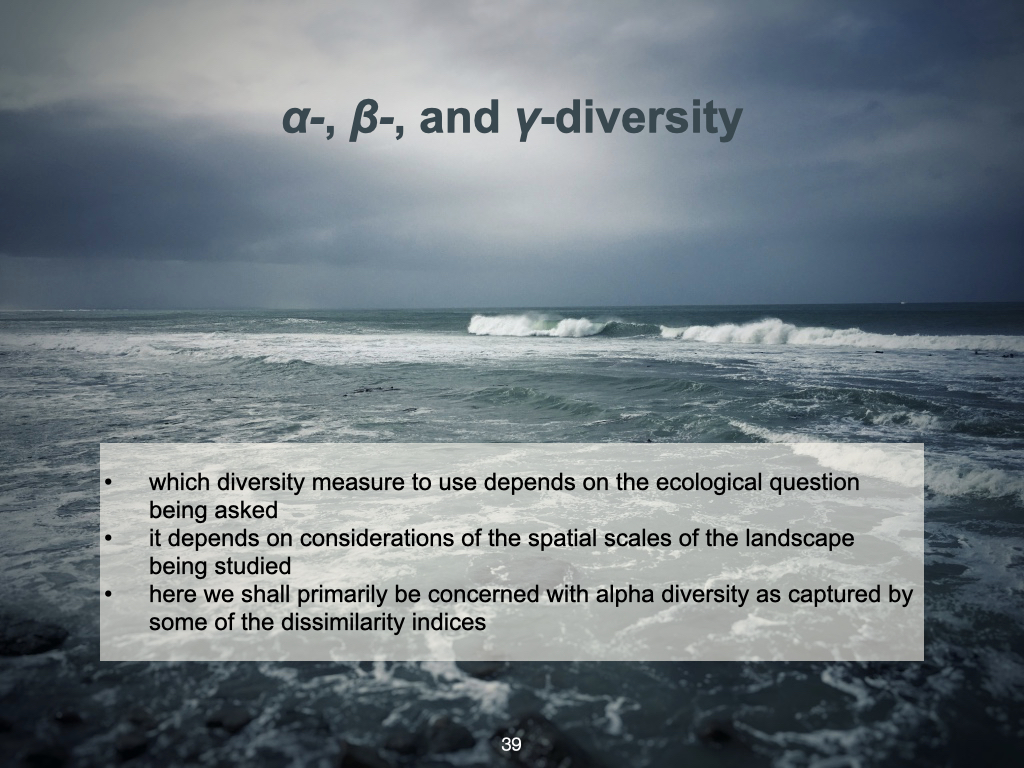
\includegraphics[width=0.8\linewidth]{../images/BDC334/BDC334-039.jpeg}
\caption*{Slide 39}
\end{figure}

Which of these various different measurements of diversity we use, is
going to depend on your specific question (Slide 39). As you are
ecologists, or training to become ecologists, it is up to you to decide
what the question is that you wish to ask about the landscape you want
to study. One day, when you are professional ecologists, you will decide
which landscape to study, for what reason, what the total extent will
be, and whether a small \(2\;\mathrm{m} \times 2\;\mathrm{m}\) quadrat,
or a smaller \(30\;\mathrm{cm} \times 30\;\mathrm{cm}\) quadrat, would
be more appropriate for your sampling.

You will define the scales at which you apply the terms alpha, beta, and
gamma diversity, as well as the amount of variation within the total
landscape --- the area for which you calculate gamma diversity. The
variation within that landscape is beta diversity, but again, the choice
of spatial scale and focus is dependent on you, as researchers.

So, in designing any particular research project, there are many
questions around spatial scales that you must consider as part of the
experimental design process. This will result in the structure within
which you sample the environment --- a structured way to obtain the data
you need to make a proper assessment of ecological diversity.

\section{Overview of Diversity
Indices}\label{overview-of-diversity-indices}

\begin{figure}[ht]
\centering
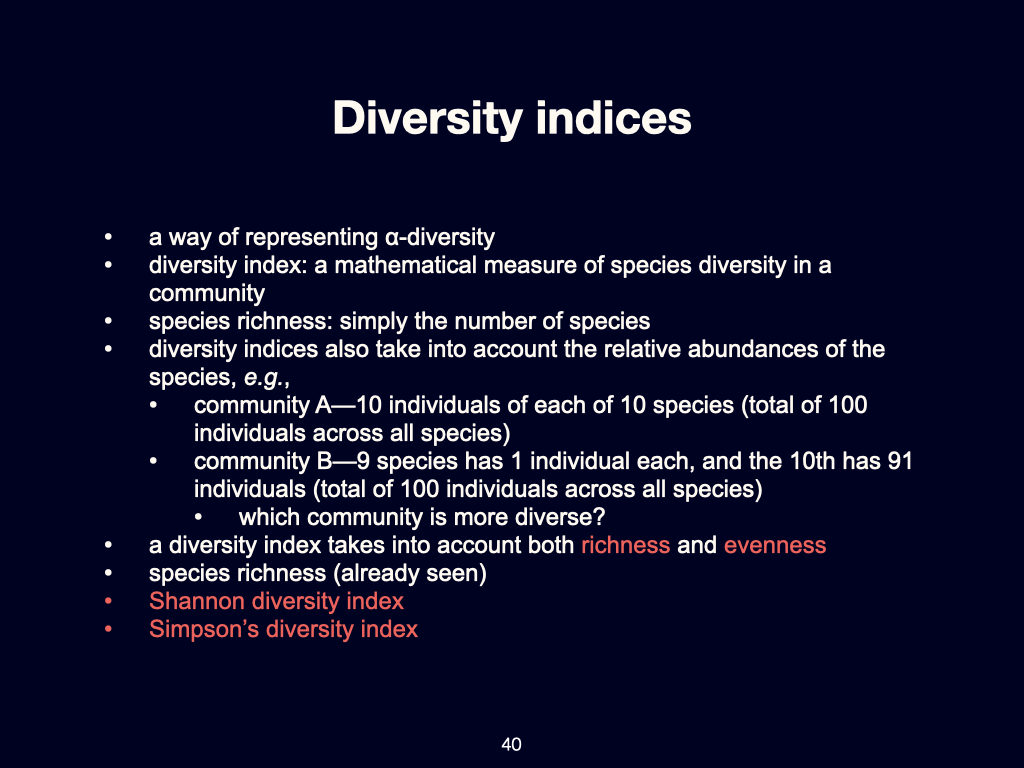
\includegraphics[width=0.8\linewidth]{../images/BDC334/BDC334-040.jpeg}
\caption*{Slide 40}
\end{figure}

The diversity indices, as I have mentioned before, are simply ways of
representing species diversity (Slide 40). Let us return to alpha
diversity as an example. The simplest way to measure alpha diversity is
to calculate species richness --- that is, to record how many species
are present within a small sampling unit.

However, landscapes are not only defined by a simple list of species. Of
course, it is important whether a species is present or absent, but
another essential consideration is how much of each species is present
in the sample. For example, consider two communities, two different
habitats. Both have 10 species present, so in terms of species richness,
both community A and community B are equal: \(10\) and \(10\).

But in community A, there are \(10\) individuals of every species --- an
even distribution. In community B, there is only \(1\) individual of
each species from \(1\) to \(9\), but species \(10\) has \(91\)
individuals present. So, although both communities have identical lists
of species, they differ substantially in terms of the abundances of
those species.

This is where diversity indices for alpha diversity become important.
These indices take into account both the number of species (species
richness) and the relative abundance, or number of individuals, of each
species. The two most common ways we represent or express diversity as a
function of species richness and abundance are through diversity
indices: the Shannon diversity index and the Simpson's diversity index.
Each of these has a particular equation to calculate their values, but
the software we use typically performs the computation for you.

\section{Calculating Diversity
Indices}\label{calculating-diversity-indices}

Some of the exercises that you will tackle later will require you to
calculate these indices by hand. Unfortunately, this year, due to the
lockdown and not being able to use the university's computer labs, you
will need to perform these calculations manually. In every other year,
you would have used standard software for these.

I shall give you, as an exercise later in the week, some sets of
diversity data and ask you to calculate these indices yourselves, by
hand.

\begin{figure}[ht]
\centering
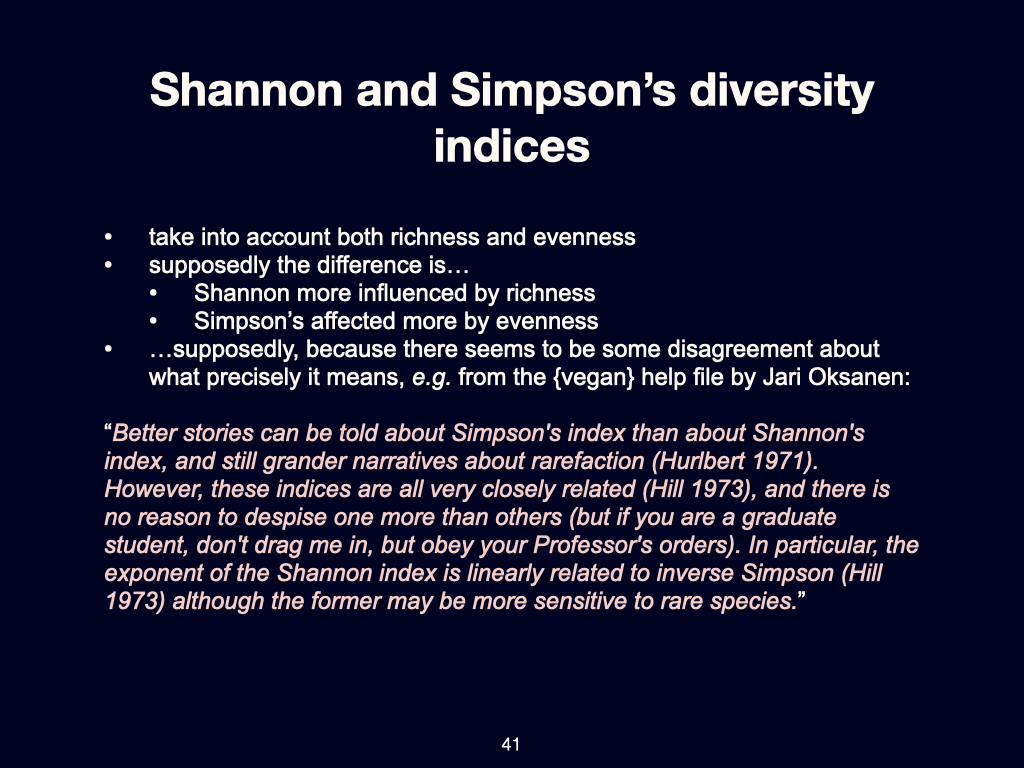
\includegraphics[width=0.8\linewidth]{../images/BDC334/BDC334-041.jpeg}
\caption*{Slide 41}
\end{figure}

Now, the two indices --- Shannon's and Simpson's --- differ slightly,
although there is ongoing debate about precisely how much they differ
and in what aspect (Slide 41). Many people say that Shannon's diversity
index favours species richness. That is, it puts more emphasis on
place-to-place differences that result from the number of species
present. Simpson's index, by contrast, is said to be more important in
contexts where the number of individuals per species varies greatly
across the landscape.

But as I noted, there is much debate as to which index is preferable.
There is even a slide, or paragraph from the software we use, which
states: ``Better stories can be told about Simpson's index than about
Shannon's index, and still grander narratives about rarefaction.''
(Rarefaction is yet another way of considering species diversity.)
However, all these indices are closely related, and there is no reason
to prefer or despise one over the others. The same paragraph, however,
gives a word of advice: ``If you are a graduate student, do not drag me
in, but obey your professor's order.'' So, at the end of the day ---
whether you use Simpson's or Shannon --- much will depend on the
preferences of your future supervisors. Everyone has their own opinions.
In my personal view, it makes little difference; they are, in fact,
linearly related to one another. Still, please do listen to what your
supervisor says.

\section{Structure of Diversity Data}\label{structure-of-diversity-data}

\begin{figure}[ht]
\centering
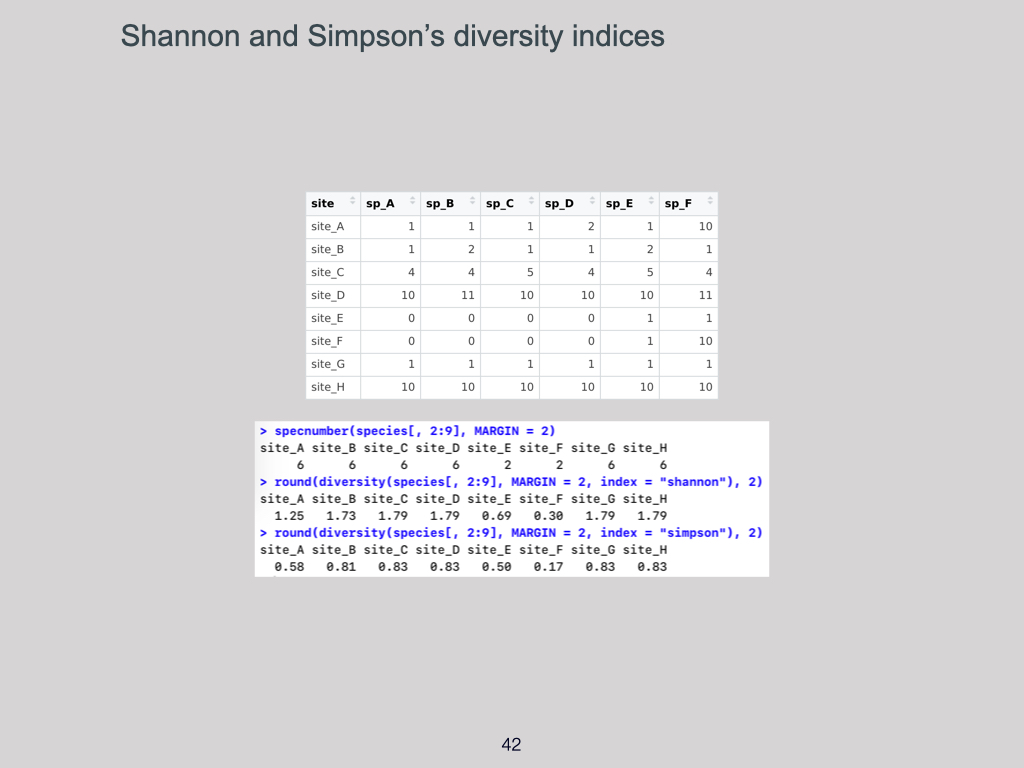
\includegraphics[width=0.8\linewidth]{../images/BDC334/BDC334-042.jpeg}
\caption*{Slide 42}
\end{figure}

Let us return to the matter of how these indices are calculated. The
essential thing to learn now is how your data should be structured when
entering it into the computer for analysis.

Typically, we enter all the various places (the sites or quadrats) along
the rows, and the species --- by name --- along the columns (Slide 42).
The numbers in the table represent the abundance: for example, species A
at site A, there is one; species B at site C, there are four; species B
at site D, there are eleven; and so on.

Species richness is easy to calculate using this structure: for any
site, simply count how many columns (species) contain a positive number.
For instance, site A might have six species present (species richness =
\(6\)), as might site B. Importantly, the abundance --- that is, the
actual number of individuals per species --- is not considered when
calculating species richness.

But the Shannon-Wiener index does take these abundances into account, as
does the Simpson's index. For example, the Simpson's index emphasises
sites with higher evenness of abundance between species: if, for an
area, only two species are present and the others have zero, you will
get a low Simpson's diversity value. Conversely, if the abundances are
more evenly distributed among species, the Simpson index value is
higher.

Evenness refers to how similar the abundances of the different species
are: a site where all species are represented by roughly equal numbers
of individuals has high evenness; a site where one species dominates and
the rest are rare has low evenness.

Please familiarise yourselves with the process of working out these
indices using sample tables. I will provide some examples for you to
work through. Normally, we would use software --- ``R'' in our case ---
to calculate these indices, but for now, manual calculation will
suffice. If you go on to Honours next year, you will have the
opportunity to catch up with the R software then.

\section{Application to South Africa: Example Using Simpson's
Index}\label{application-to-south-africa-example-using-simpsons-index}

\begin{figure}[ht]
\centering
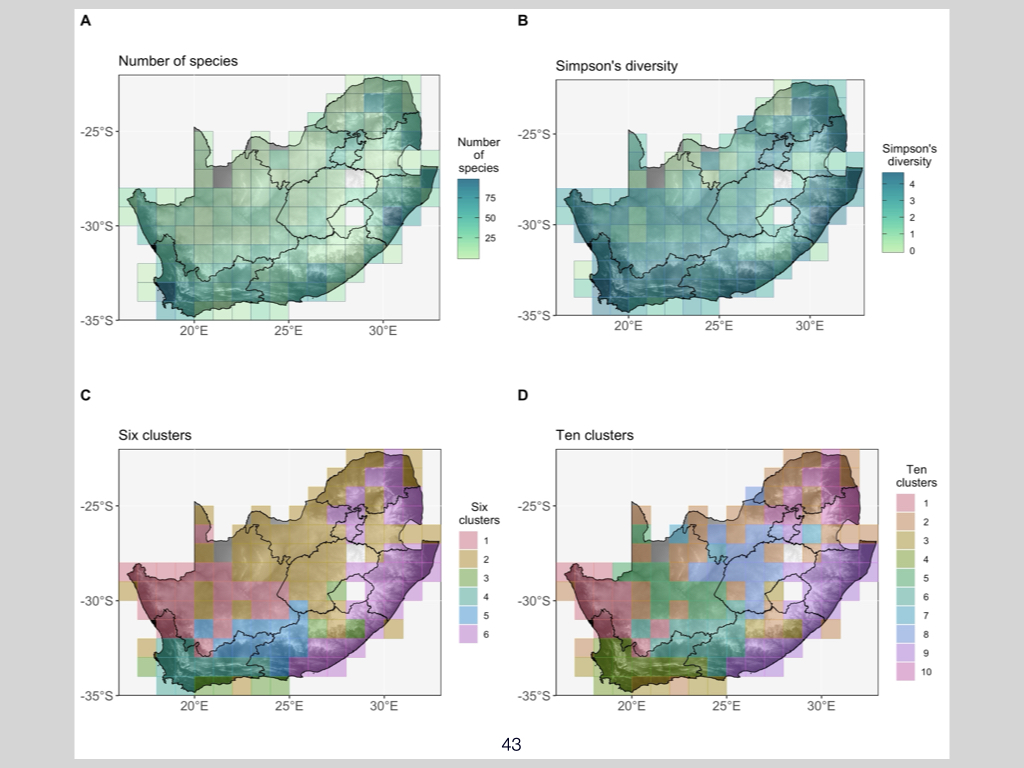
\includegraphics[width=0.8\linewidth]{../images/BDC334/BDC334-043.jpeg}
\caption*{Slide 43}
\end{figure}

Here is an example where I have applied Simpson's diversity index to
various places in South Africa (Slide 43). If South Africa represents
the area for which we define gamma diversity, then each square or
quadrant on the map represents an area where we calculate alpha
diversity.

The number of crickets present per area has been plotted across South
Africa, and you can see that dartker colours indicate areas with higher
cricket abundance. These numbers --- or rather, the diversity indices
calculated from them --- show substantial variation across the country.
The most diverse areas appear in Limpopo and along the coast,
particularly in northern KwaZulu-Natal, where evenness is also highest.

Whereas in other areas, especially inland, there are many more locations
with low diversity and a few with significantly more individuals of
particular species. Along the coast, most species are fairly evenly
represented.

With this sort of information, we can begin to classify South Africa
into regions that share similar levels or patterns of diversity, in
terms of both the type and presence/abundance of species. This is the
value of using these diversity indices --- a starting point for further
analyses. The kind of calculation I have described here is known as
clustering analysis. This will not be covered this year, but this is
just to show you an example of potential future applications.

Such analyses can be useful on their own, as they visually reveal the
different diversity patterns present across a region.

\section{Reading and Administrative
Notes}\label{reading-and-administrative-notes}

\begin{figure}[ht]
\centering
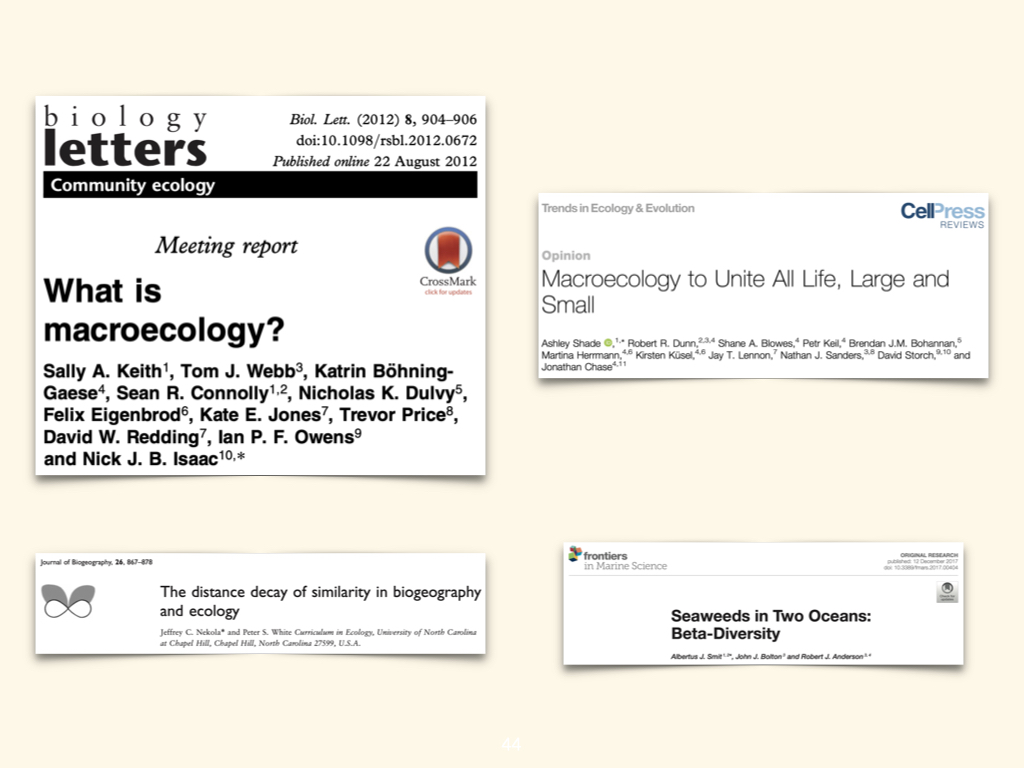
\includegraphics[width=0.8\linewidth]{../images/BDC334/BDC334-044.jpeg}
\caption*{Slide 44}
\end{figure}

A reminder: I have given you two papers to read --- ``What is
Macroecology?'' and ``Macroecology to Unite All Life, Large and Small''
(Slide 43). You should have read and understood both, as last week was
allocated for that reading. The assumption is that you now understand
everything covered in those papers, otherwise you would have asked by
now. That opportunity has passed.

For this week, you have additional reading around ecological gradients:
(1) ``Distance, Decay of Similarity in Biogeography and Ecology'' by
Jeffrey Nicola, and (2) ``Seaweeds in Two Oceans: Beta Diversity'' by
myself. Please read these two papers this afternoon.

On Friday, or Thursday, you are welcome to make an appointment with me,
in groups of three or four or more, if you have any questions about
these two papers. Failing to ask me questions by Thursday will imply
that you understand everything, and I am then free to ask you anything
from these papers in future tests and exams.

\chapter{Multivariate Data}\label{sec-lect5}

\begin{tcolorbox}[enhanced jigsaw, colback=white, bottomrule=.15mm, opacitybacktitle=0.6, arc=.35mm, opacityback=0, left=2mm, coltitle=black, colframe=quarto-callout-note-color-frame, breakable, bottomtitle=1mm, toptitle=1mm, toprule=.15mm, titlerule=0mm, leftrule=.75mm, title=\textcolor{quarto-callout-note-color}{\faInfo}\hspace{0.5em}{BCB743}, colbacktitle=quarto-callout-note-color!10!white, rightrule=.15mm]

This material must be reviewed by BCB743 students in Week 1 of
Quantitative Ecology.

\end{tcolorbox}

\begin{tcolorbox}[enhanced jigsaw, colback=white, bottomrule=.15mm, opacitybacktitle=0.6, arc=.35mm, opacityback=0, left=2mm, coltitle=black, colframe=quarto-callout-note-color-frame, breakable, bottomtitle=1mm, toptitle=1mm, toprule=.15mm, titlerule=0mm, leftrule=.75mm, title=\textcolor{quarto-callout-note-color}{\faInfo}\hspace{0.5em}{Also see:}, colbacktitle=quarto-callout-note-color!10!white, rightrule=.15mm]

Accompany your reading of in this chapter with the material in
\href{Lab-01-introduction.html}{Lab 1}, \href{Lab-02b-env_dist.html}{Lab
2b}, and \href{Lab-03-biodiversity.html}{Lab 3}.

\end{tcolorbox}

\chapter*{Lecture 5a}\label{lecture-5a}
\addcontentsline{toc}{chapter}{Lecture 5a}

\section{Introduction}\label{introduction}

We're going to look at the multivariate nature of ecological data. Last
week, I spoke about how to go about collecting samples of species from a
particular landscape or habitat, using the UWC Nature Reserve as an
example.

\section{Types of Ecological Data}\label{types-of-ecological-data}

\begin{figure}[ht]
\centering
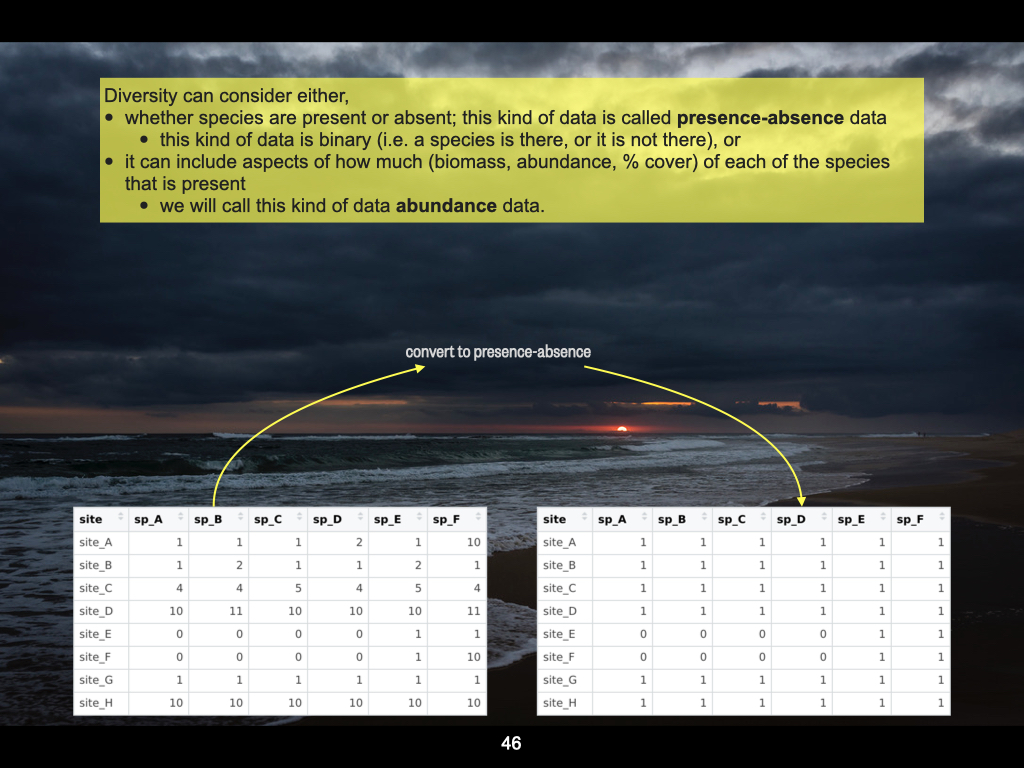
\includegraphics[width=0.8\linewidth]{../images/BDC334/BDC334-046.jpeg}
\caption*{Slide 46}
\end{figure}

The kinds of data we can obtain from a place like the UWC Nature Reserve
include a collection of quadrats, which I've labelled here as `site A'
to `site H' --- so there are eight of them (Slide 46). At each site, for
every one of the quadrats we place on the landscape, we count the number
of species present.

For instance, in this example, site A has six species present, while
site E has only two species present. The zeros indicate that none of
those particular species were present.

Now, these two sets of data tables --- the one on the left and the one
on the right --- are more or less identical in that they represent the
same samples. The difference is that the table on the left, in addition
to indicating whether a species is present (a `1') or absent (a `0'),
also shows, if a species is present at a particular site, how much of
the species is present --- for example, its abundance, biomass,
percentage cover, and so on. If it is not present, there will be a zero.
Wherever there is a `1' on this particular table, on the left, the ones
could be any number greater than zero, indicating how much of that
species is present.

The table on the right simply shows a `1' to indicate presence and a `0'
for absence. This is what we call presence-absence data.

So, the left-hand data type is called abundance data, and the right-hand
side is presence-absence data. On the right, we only know whether a
species is there or not. On the left, if a species is present, we also
know how much of it is present. This is a critical distinction you need
to keep in mind.

You'll encounter both of these data types as we progress through the
module.

\section{Determining Similarity Between
Sites}\label{determining-similarity-between-sites}

Today, the goal is to determine how similar various places are to each
other, especially regarding their species composition.

Let's refer back to the earlier slide. We can see that certain sites are
more similar to others but in different ways. In the first instance, two
sites could be similar because they share the same species. For example,
both site A and site B each have species A, B, C, D, E, and F. The
difference between site A and site B is primarily due to species F,
where site A has much more of species F compared to site B.

So, overall, there are two main reasons why locations can be similar or
different. The first is that they share the same species, and the second
is that, even if they share species, the abundance of each species is
unequal; one place may have more individuals of a species, while another
has fewer, and so on.

Another kind of difference comes when, say, comparing site D and site E:
site E may have only two species that are also present in site D,
whereas site D has four other species present not found in site E. Sites
might therefore share some species, differ in others, or have uneven
abundances of shared species.

So, as an ecologist, it's your job to determine why particular places
are different from one another in terms of community structure.

\section{Reasons for Differences in
Communities}\label{reasons-for-differences-in-communities}

Communities differ from place to place for at least three reasons:

\begin{enumerate}
\def\labelenumi{\arabic{enumi}.}
\item
  \textbf{Environmental differences:} The environment may be different
  at the two places. For example, one environment may be too warm,
  excluding species that prefer colder temperatures. Environmental
  differences may explain why community compositions vary.
\item
  \textbf{Unmeasured influences:} If it's not due to the environment (or
  not the part we measured), there might be other unaccounted or unknown
  influences. These are unmeasured factors for which we can pose
  hypotheses for further research and data collection.
\item
  \textbf{Random noise:} Alternatively, differences may simply be due to
  random noise, stochastic events, or measurement inaccuracies that
  obscure genuine patterns.
\end{enumerate}

So, understanding community differences involves asking whether
differences are due to measurable environmental factors, unknown
influences, or just random variation. Analysing the data helps narrow
down which of these is most likely.

\section{Data Representation: Distance, Similarity, and Dissimilarity
Matrices}\label{data-representation-distance-similarity-and-dissimilarity-matrices}

\begin{figure}[ht]
\centering
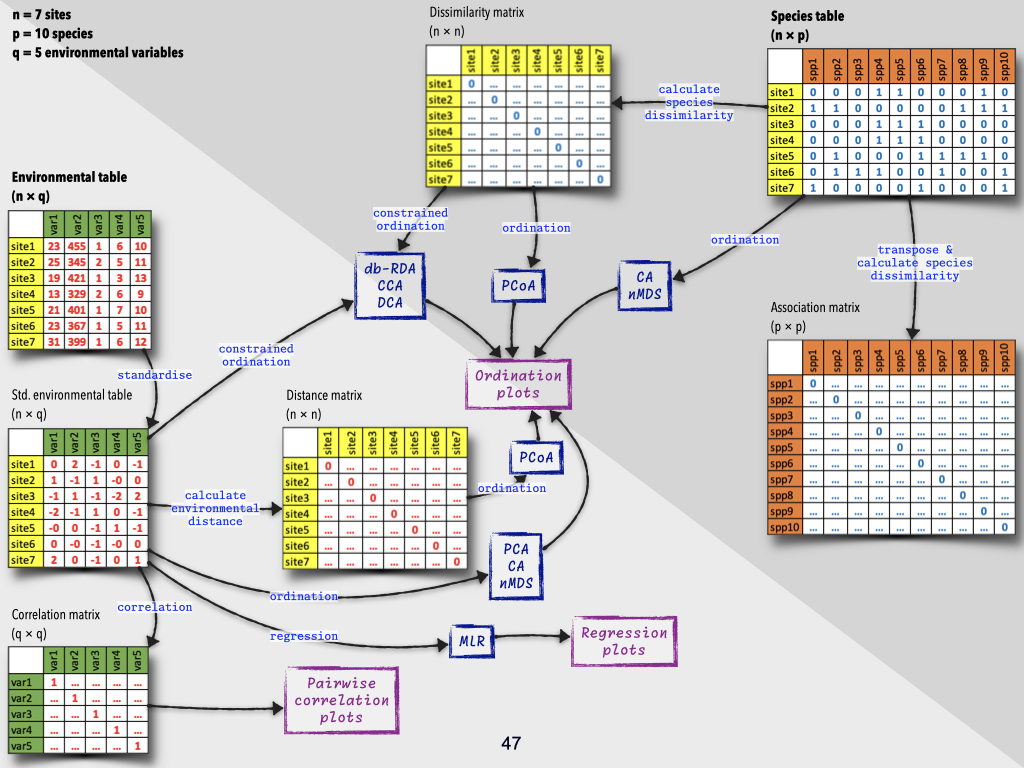
\includegraphics[width=0.8\linewidth]{../images/BDC334/BDC334-047.jpeg}
\caption*{Slide 47}
\end{figure}

\begin{figure}[ht]
\centering
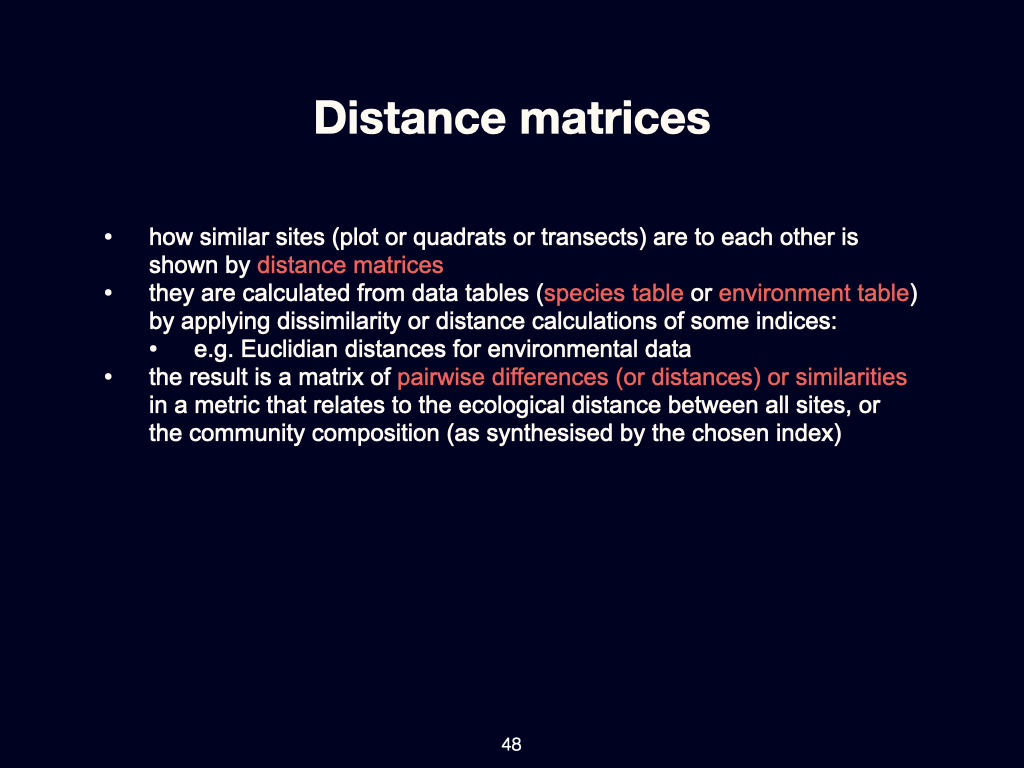
\includegraphics[width=0.8\linewidth]{../images/BDC334/BDC334-048.jpeg}
\caption*{Slide 48}
\end{figure}

\begin{figure}[ht]
\centering
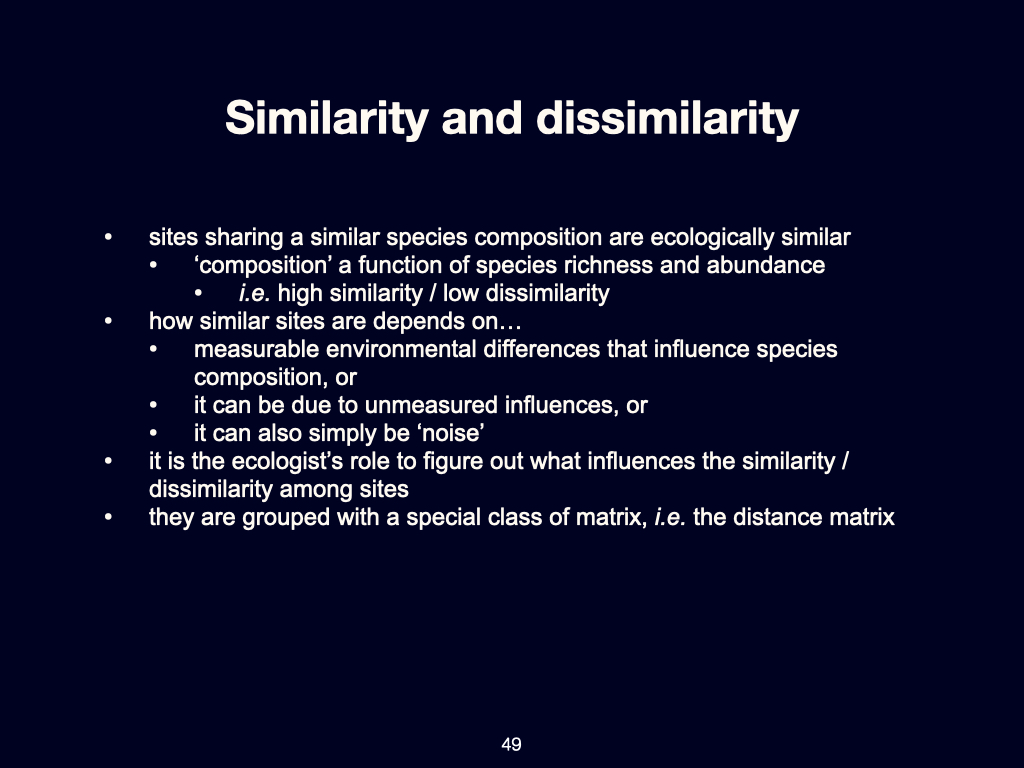
\includegraphics[width=0.8\linewidth]{../images/BDC334/BDC334-049.jpeg}
\caption*{Slide 49}
\end{figure}

\begin{figure}[ht]
\centering
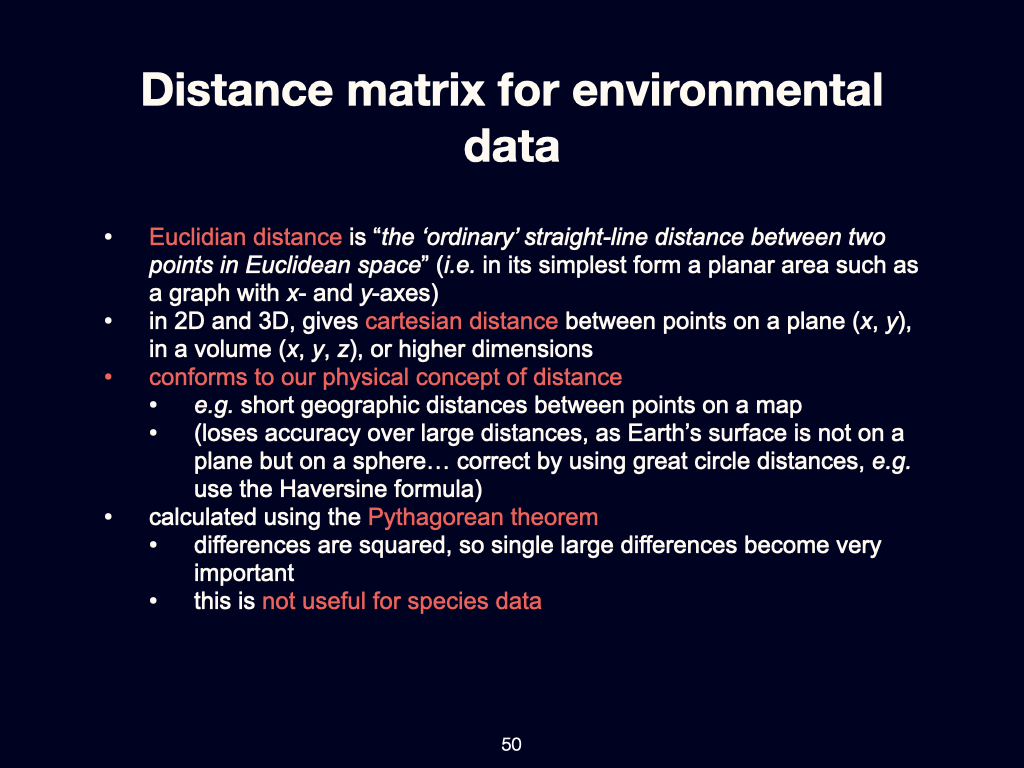
\includegraphics[width=0.8\linewidth]{../images/BDC334/BDC334-050.jpeg}
\caption*{Slide 50}
\end{figure}

\begin{figure}[ht]
\centering
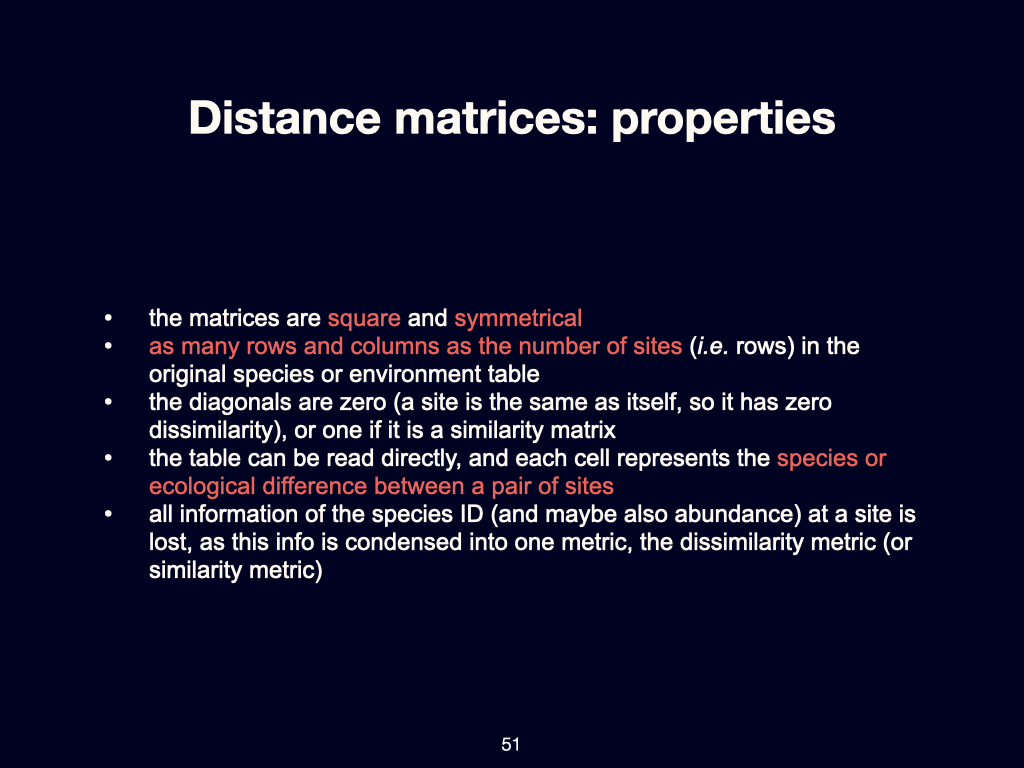
\includegraphics[width=0.8\linewidth]{../images/BDC334/BDC334-051.jpeg}
\caption*{Slide 51}
\end{figure}

The different kinds of data for comparing places --- be that
similarities in species presence or differences in environmental
variables --- can be represented as distance matrices, more
specifically, similarity or dissimilarity matrices (Slides 47-51).

When discussing environmental or species differences, we use distinct
types of matrices. Broadly, each matrix is a distance matrix, but the
way we calculate distance depends on the type of data.

\begin{itemize}
\tightlist
\item
  For \textbf{environmental data} (e.g., temperature, humidity, soil
  type), we use an \textbf{actual distance measure}, typically the
  \textbf{Euclidean distance}.
\item
  For \textbf{species composition data} (abundance or presence-absence),
  instead of Euclidean distance, we use similarity/dissimilarity indices
  such as \textbf{Bray-Curtis}, \textbf{Sørensen}, or \textbf{Jaccard
  indices}.
\end{itemize}

So, just to recap: environmental data includes things like temperature,
humidity, depth, light intensity, soil and nutrient composition, and so
on; all the things we measure about the environment which might explain
community differences. Species data is what species are present or
absent, and potentially, how much of each species is present.

From both, we can calculate distance matrices:

\begin{itemize}
\tightlist
\item
  Environmental data \(\rightarrow\) \textbf{Euclidean distance}
\item
  Species data \(\rightarrow\) \textbf{Bray-Curtis}, \textbf{Sørensen},
  \textbf{Jaccard}, etc.
\end{itemize}

These matrices represent the pairwise differences between each pair of
sites.

\section{Pairwise Comparisons}\label{pairwise-comparisons}

By `pairwise', I simply mean comparing every site to every other site.

So, for example, site A is compared to site B, site A is compared to
site C, site A is compared to site D, site E to site C, site G to site
F, and so forth. For each pair, we calculate how similar or dissimilar
they are, for both environmental and species data, using the appropriate
metric.

There are many dissimilarity indices you can use for species data, and
you'll see some examples in class. But the principle is always the same:
you calculate the similarity or difference for every possible
combination of pairs.

The result is a matrix where every entry shows the similarity or
difference between one site and another.

\section{Calculating Euclidean
Distance}\label{calculating-euclidean-distance}

\begin{figure}[ht]
\centering
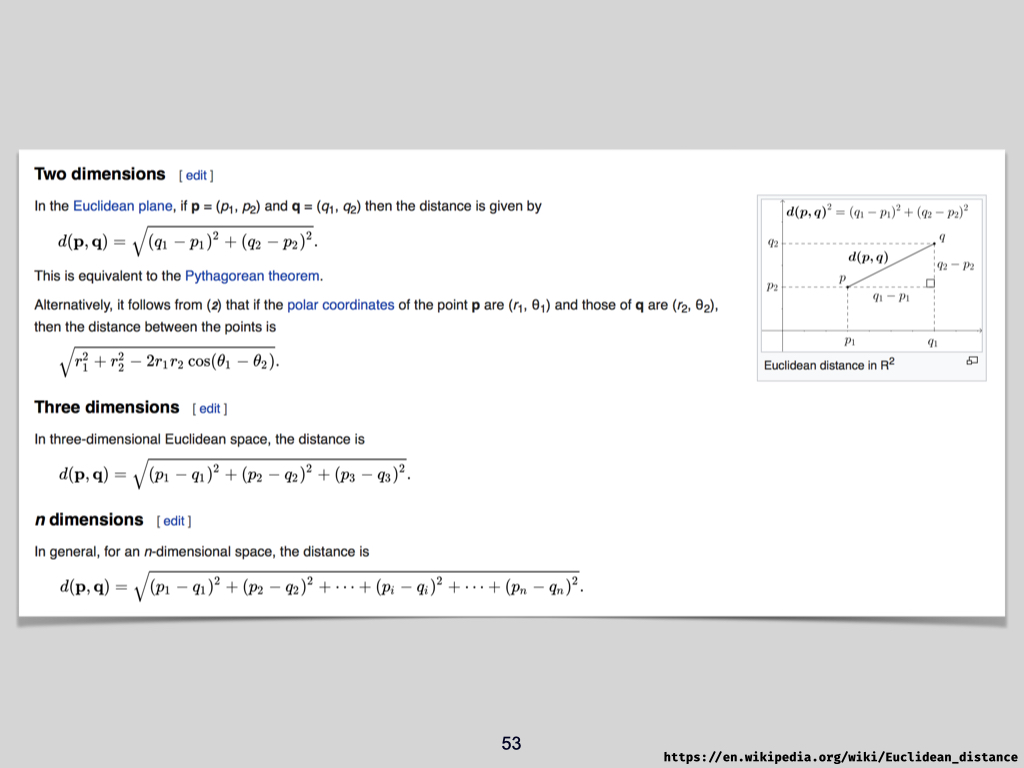
\includegraphics[width=0.8\linewidth]{../images/BDC334/BDC334-053.jpeg}
\caption*{Slide 53}
\end{figure}

So, how do we actually calculate Euclidean distance, which is the main
way we measure how different our environmental samples are from each
other (Slide 53)?

Euclidean distance is the direct, straight-line measure between two
points. Imagine plotting two points on a coordinate plane with x- and
y-axes; each point has an x-coordinate and a y-coordinate. The
straight-line, or shortest, distance between the two points is the
Euclidean distance. The unit of this distance is the same as the unit
used for the axes.

If both the x- and y-axes are measured in centimetres, then the diagonal
(shortest) distance between your two points will also be measured in
centimetres. This is sometimes called Cartesian distance.

You can extend this idea to three dimensions --- for example, x, y, and
z --- with the Euclidean distance representing the straight line between
two points in three-dimensional space.

But you are not limited to two or three dimensions. Ecological data is
often `multi-dimensional' because for each site we may have ten, twenty,
or even a hundred environmental variables (dimensions) measured. Humans
can't visualise more than three dimensions, but mathematically,
calculating the Euclidean distance between points with many dimensions
works just the same.

Euclidean distance aligns with our intuitive sense of ``distance'' when
we're talking about physical or geographic space, but in the context of
ecological data, it reflects how different or similar environmental
samples are, based on the variables we've measured.

\section{Applying the Pythagorean
Theorem}\label{applying-the-pythagorean-theorem}

To calculate Euclidean distance, we use the Pythagorean theorem, which
you should remember from secondary school mathematics.

Suppose you have a two-dimensional graph (your y-axis is vertical,
x-axis is horizontal) and two points, P and Q.

\begin{itemize}
\tightlist
\item
  Point P is at coordinates \((P_1, P_2)\).
\item
  Point Q is at coordinates \((Q_1, Q_2)\).
\end{itemize}

To calculate the straight-line (Euclidean) distance between P and Q:

\begin{enumerate}
\def\labelenumi{\arabic{enumi}.}
\tightlist
\item
  Find the difference in \(x\) between \(Q\) and \(P\): \(Q_1 - P_1\).
\item
  Find the difference in \(y\) between \(Q\) and \(P\): \(Q_2 - P_2\).
\item
  Square both differences: \((Q_1 - P_1)^2 + (Q_2 - P_2)^2\).
\item
  Take the square root: \(\sqrt{(Q_1 - P_1)^2 + (Q_2 - P_2)^2}\).
\end{enumerate}

That's your Euclidean distance.

If you have three dimensions, say \(x, y,\) and \(z\), you simply extend
the equation:

\[
\sqrt{(Q_1 - P_1)^2 + (Q_2 - P_2)^2 + (Q_3 - P_3)^2}
\]

And for \(n\) dimensions, you generalise:

\[
\sqrt{\sum_{i=1}^{n} (Q_i - P_i)^2}
\]

So, it's straightforward. For as many variables as you have, just extend
the formula, square the differences for each corresponding variable, sum
them, and take the root.

\section{Worked Example}\label{worked-example}

\begin{figure}[ht]
\centering
\includegraphics[width=0.8\linewidth]{../images/BDC334/BDC334-054.jpeg}
\caption*{Slide 54}
\end{figure}

Imagine our sites and their coordinates. Each site has an \(x\) and
\(y\) coordinate (Slide 54). For instance:

\begin{itemize}
\tightlist
\item
  Site A: \((2, 1)\)
\item
  Site B: \((3, 5)\)
\end{itemize}

The difference in the \(x\) dimension between A and B is \(3 - 2 = 1\),
and in the \(y\) dimension is \(5 - 1 = 4\).

So the Euclidean distance between A and B is:

\[
\sqrt{1^2 + 4^2} = \sqrt{1 + 16} = \sqrt{17} \approx 4.123
\]

You would repeat this process for every pair of sites, filling in the
matrix of pairwise distances.

\begin{figure}[ht]
\centering
\includegraphics[width=0.8\linewidth]{../images/BDC334/BDC334-055.jpeg}
\caption*{Slide 55}
\end{figure}

If you had more dimensions, you'd follow the same logic, adding more
squared differences and including them under the square root (Slide 55).

You can see that pairs of points which are close in (two-dimensional)
space have small values in the distance matrix, while those farther
apart have larger values.

\section{Multidimensional Ecological
Distance}\label{multidimensional-ecological-distance}

\begin{figure}[ht]
\centering
\includegraphics[width=0.8\linewidth]{../images/BDC334/BDC334-056.jpeg}
\caption*{Slide 56}
\end{figure}

\begin{figure}[ht]
\centering
\includegraphics[width=0.8\linewidth]{../images/BDC334/BDC334-057.jpeg}
\caption*{Slide 57}
\end{figure}

How does this apply to ecological data, which might not be spatial at
all? Well, each environmental variable --- temperature, depth, light
intensity, pH, CO\(_2\) content, soil condition, whatever you're
measuring --- can be treated as one dimension (Slides 56-57).

So each site becomes a point in this multi-dimensional space, and the
environmental distance between two sites is simply calculated using the
Euclidean formula: for example, with environmental variables
temperature, depth, and light, the ecological distance between site A
and site B would be:

\[
\sqrt{(T_A - T_B)^2 + (D_A - D_B)^2 + (L_A - L_B)^2}
\]

Where \(T\) is temperature, \(D\) is depth, \(L\) is light.

If you add more variables, simply keep extending the formula.

\section{Take-Home Message}\label{take-home-message}

This is why we say ecological data has a multivariate or
multidimensional nature. Whether we're using environmental variables or
species abundances or presences, we're working in a space with as many
dimensions as we have types of data measured.

For environmental data, we use \textbf{Euclidean distance} to build
these matrices.

Remember: \textbf{Euclidean distance is appropriate for environmental
(quantitative) data. Do not apply it to species data --- you shouldn't.}
For species data (particularly presence/absence or abundance), use
\textbf{Bray-Curtis, Sørensen, Jaccard}, or other appropriate indices.

So, in summary, the multivariate nature of ecological data comes from
the multiple dimensions contained in our data --- each dimension being
an environmental characteristic or a species measure. We express the
similarity or difference between sites through pairwise comparison,
using the appropriate formula to build our distance (or
similarity/dissimilarity) matrices. These matrices are the foundation
for further analyses you'll be doing throughout this module.

\chapter*{Lecture 5b}\label{lecture-5b}
\addcontentsline{toc}{chapter}{Lecture 5b}

\section{Applying Euclidean Distances to Environmental
Variables}\label{applying-euclidean-distances-to-environmental-variables}

Right, so you understand now how to use Euclidean distances to calculate
for us how different places are in terms of ecological conditions, or
more specifically, the environmental conditions present there. We apply
the theorem of Pythagoras to environmental data, where each one of the
environmental variables becomes a dimension in our analysis. In this
instance, think of temperature, depth, and light. Temperature would be
dimension one, depth would be dimension two, and light would be
dimension three. So, we have three dimensions in our equation.

It does not matter what order they are arranged in; it is completely
arbitrary. But because all of these feature together, simultaneously, in
some kind of combined measurement of how different the environment is
from place to place, the specific units actually fall away. In this
calculation, the values in environmental units become meaningless --- it
becomes just `ecological distance'. That is simply how it is.

\section{Standardising Environmental
Data}\label{standardising-environmental-data}

\begin{figure}[ht]
\centering
\includegraphics[width=0.8\linewidth]{../images/BDC334/BDC334-059.jpeg}
\caption*{Slide 59}
\end{figure}

Now, here is another example. It's a similar kind of example to what we
looked at before, but you will notice that there is a new table inside
here (Slide 59). The reason we have this new table is because we have
standardised the data. It is actually the same data, but the values are
now very different. For example, the values for pH are recognisable pH
numbers, more or less close to neutral. We have moderately aerated
water, fairly moderate temperatures as well, and a very shallow kind of
freshwater environment. All of these values look familiar because these
are things you have probably come across before, and intuitively, you
can understand them.

However, when you look at the standardised data, you'll see that these
numbers almost look --- well, not random, they're definitely not random
--- but to the untrained eye, if you do not know why the numbers look
the way they do, it might as well look random to you. What is important
here is that we have standardised the data. We have transformed the raw
data into standardised data.

\section{Why Standardise?}\label{why-standardise}

The reason why we standardise things is this: if we do not, then
variables like temperature are going to become far more important in
influencing the environmental distances. This is because the units and
the values of temperature are much larger than, say, the values for
depth.

So, in our previous example, where we had variables like \(x\) and
\(y\), because \(x\), \(y\), and \(z\) were all measured in, say,
centimetres, there was no need to transform the data, since the values
are comparable in magnitude. But here, the magnitude of values is very
different between the variables. Temperature is measured in degrees
Celsius, depth is measured in metres. The units cannot be compared to
each other because they are entirely different measures.

Therefore, in order to rescale them --- so that temperature does not
become more important in the calculation than depth or any other
variable --- we standardise them.

\section{How Standardisation Works}\label{how-standardisation-works}

\begin{figure}[ht]
\centering
\includegraphics[width=0.8\linewidth]{../images/BDC334/BDC334-060.jpeg}
\caption*{Slide 60}
\end{figure}

\begin{figure}[ht]
\centering
\includegraphics[width=0.8\linewidth]{../images/BDC334/BDC334-061.jpeg}
\caption*{Slide 61}
\end{figure}

Standardising the data essentially scales the mean and the standard
deviation. If you transform your raw data into standardised data, the
property of this data is such that:

\begin{itemize}
\tightlist
\item
  The mean of the standardised data is \(0\).
\item
  The standard deviation is \(1\).
\end{itemize}

So, you rescale the data from the raw measurement units into this
standardised format. This means that, in your standardised data, the
average value of temperature or depth, for example, will be exactly
\(0\), and all variables are now comparable in magnitude. Temperature
will no longer have values with an average of about \(12\), and depth
will no longer have an average of around \(1.6\) or \(1.7\), but all
means will be \(0\) (Slides 60-61).

As a result, temperature does not become the overriding factor in our
Euclidean distance calculation. When we calculate the Euclidean distance
between sites, all the environmental variables have exactly the same
weight in the calculation.

\section{Calculating Euclidean Distances after
Standardisation}\label{calculating-euclidean-distances-after-standardisation}

So, we always standardise raw environmental data so that the units of
measurement become comparable, and one variable does not become far more
influential in the calculation compared to another. Once standardised,
we can then apply the Euclidean distance calculation properly.

I'll show you the calculation or the equation you will use to
standardise your data. It is not very tricky at all; it's
straightforward to do in Excel, or even just with a calculator ---
nothing complicated there.

\section{Species Data: A Different Kind of
Distance}\label{species-data-a-different-kind-of-distance}

\begin{figure}[ht]
\centering
\includegraphics[width=0.8\linewidth]{../images/BDC334/BDC334-062.jpeg}
\caption*{Slide 62}
\end{figure}

So far, we have spoken about environmental data. But we can also know
what the difference is in species composition from place to place. To do
that, we no longer use environmental data but data on whether species
are present or not, so-called presence--absence data, or abundance data
if available (Slide 62).

In this case, we do not use the Euclidean distance calculation. The
Euclidean distance relies on the Pythagorean theorem. However, when
calculating the distance between sites in terms of which species are
present, or their abundance, we must use a different measure.

Here, we use indices such as the Bray--Curtis, Jaccard, or Sørensen
index. These are used instead of Euclidean distance to calculate how
different the species assemblages are from one another.

\section{Applying the Indices to Species
Data}\label{applying-the-indices-to-species-data}

Here you would have species data. So, suppose we have sites, let's say
sites \(1\) to \(10\). These are the same sites as before. As I said in
an earlier lecture, the rows always tell you which places you have
sampled (Slides 63-66). So, for example, ten replicates within the UWC
Nature Reserve, each one identified by an integer --- quadrat \(1\),
\(2\), \(3\), and so on, up to \(10\).

\begin{figure}[ht]
\centering
\includegraphics[width=0.8\linewidth]{../images/BDC334/BDC334-063.jpeg}
\caption*{Slide 63}
\end{figure}

\begin{figure}[ht]
\centering
\includegraphics[width=0.8\linewidth]{../images/BDC334/BDC334-064.jpeg}
\caption*{Slide 64}
\end{figure}

\begin{figure}[ht]
\centering
\includegraphics[width=0.8\linewidth]{../images/BDC334/BDC334-065.jpeg}
\caption*{Slide 65}
\end{figure}

\begin{figure}[ht]
\centering
\includegraphics[width=0.8\linewidth]{../images/BDC334/BDC334-066.jpeg}
\caption*{Slide 66}
\end{figure}

Within that first quadrat, you would measure all the different
environmental conditions, and, in the same place, you would also record
which species are present and, if they are present, how many of them
there are.

You would use environmental data, after standardising (for example, to
bring water hardness to a comparable range with altitude), to calculate
the Euclidean distance between every pair of sites. In this table, there
are \(11\) dimensions --- that is, \(11\) environmental variables.

For every one of the sites, you would compare every possible pair of
sites within the collection. For the species data, you then apply the
Bray--Curtis, Jaccard, or Sørensen index. I have uploaded onto iKamva a
paper which you should read. That will explain how to calculate pairwise
differences, and what the relevant index is that you should use to
compare (for example) site \(1\) to site \(2\), or site \(1\) to site
\(3\), and so on. You will need to figure that out by reading the paper.

It is a very simple procedure, which you can do by hand with a
calculator if you wish, or in Excel. That is your task.

\section{Preview: Properties of Your
Data}\label{preview-properties-of-your-data}

So, I will show you what some of the data you produce will look like.
First, let's look at some of the properties of the data that are
generated.

\chapter*{Lecture 5c}\label{lecture-5c}
\addcontentsline{toc}{chapter}{Lecture 5c}

\section{Introduction}\label{introduction-1}

This is a proper set of data taken from South Africa. This relates to
that paper you read by me, which I wrote in 2017 or so. These are the
temperature and various other data collected at different places along
our shoreline --- specifically, at \(58\) locations.

\section{Constructing Distance
Matrices}\label{constructing-distance-matrices}

So, if you consider that there are \(58\) sites, you can imagine just
how many different pairs of sites there would be if you paired every one
with every other one. If you apply that Euclidean distance calculation
to this, you end up with a big thing that looks like that. Let me put it
up in full screen and make it a bit bigger for you. This is what it is
going to look like. If you apply the calculation to the environmental
data from the \(58\) places --- applying Euclidean distance to every
possible pair --- this is the outcome: a large, dense matrix, which is,
obviously, not something you can do by hand. It would take you weeks.

An important aspect to note is that, when you do this for a species or
environment table --- a table with all the sites along the rows, and all
the environmental variables along the columns --- when you calculate the
Euclidean distance for every site, what you create is a square distance
matrix.

\section{Understanding the Distance
Matrix}\label{understanding-the-distance-matrix}

\begin{figure}[ht]
\centering
\includegraphics[width=0.8\linewidth]{../images/BDC334/BDC334-061.jpeg}
\caption*{Slide 61}
\end{figure}

This is a distance matrix, and it is square (Slide 61). Why do I say it
is square? There are \(58\) rows and \(58\) columns, running from \(1\)
up to \(58\). That is why it is a square matrix.

There is also another interesting feature --- a diagonal line running
from top left to bottom right, filled with zeros. The reason for this
is, if you compare site \(1\) with site \(1\), in terms of how different
they are, the ecological distance is zero --- because it's the same
site. Site \(1\) is site \(1\); thus, the difference in ecological space
between them is zero.

The bigger the number in the matrix entry, the more different those two
sites will be. So, if we compare site \(1\) on the \(1\)st column and
\(1\)st row, that is the diagonal. If you then compare, for instance,
the entry at column \(2\), row \(1\) --- that is the pair site \(1\) and
site \(2\). That value is the same as the value at column \(1\), row
\(2\). The matrix is symmetrical.

So, the upper right triangle (above the diagonal of zeros) will contain
exactly the same numbers as the lower left triangle (below the
diagonal). Typically, when we display these calculations, it is only
really interesting to display the lower left triangle.

\section{Key Properties of Distance
Matrices}\label{key-properties-of-distance-matrices}

There are three interesting things about a distance or dissimilarity
matrix, as used for species data:

\begin{enumerate}
\def\labelenumi{\arabic{enumi}.}
\tightlist
\item
  \textbf{It is square.} There are as many columns as rows --- \(58\) in
  this example.
\item
  \textbf{It is symmetrical.} The upper triangle is a mirror image of
  the lower triangle.
\item
  \textbf{There is a zero diagonal.} Each site compared to itself
  contains a zero, because there is no difference.
\end{enumerate}

Additionally, as you move further from site \(1\) along your
environmental gradient, these numbers increase, reflecting how different
the sites are. For example, site \(1\) compared to site \(2\) (adjacent
sites) will have a small ecological distance. Site \(1\) compared to
site \(4\) is a little bit bigger; site \(1\) compared to site \(18\) is
even bigger, and so forth, until you reach site \(1\) compared to site
\(58\), which would be at the opposite end of the gradient and will
provide the largest difference.

All these numbers tell you, for every possible pair of sites, how
different they are in ecological space.

\begin{figure}[ht]
\centering
\includegraphics[width=0.8\linewidth]{../images/BDC334/BDC334-067.jpeg}
\caption*{Slide 67}
\end{figure}

Your assignment is to calculate these matrices for yourselves (Slide
67).

\chapter{Unified Ecology}\label{unified-ecology}

\begin{tcolorbox}[enhanced jigsaw, colback=white, bottomrule=.15mm, opacitybacktitle=0.6, arc=.35mm, opacityback=0, left=2mm, coltitle=black, colframe=quarto-callout-note-color-frame, breakable, bottomtitle=1mm, toptitle=1mm, toprule=.15mm, titlerule=0mm, leftrule=.75mm, title=\textcolor{quarto-callout-note-color}{\faInfo}\hspace{0.5em}{Also see:}, colbacktitle=quarto-callout-note-color!10!white, rightrule=.15mm]

Accompany your reading of this chapter with the material presented in
\href{Lab-04-biodiversity}{Lab 4}.

\end{tcolorbox}

\chapter*{Lecture 6a}\label{lecture-6a}
\addcontentsline{toc}{chapter}{Lecture 6a}

\section{Introduction}\label{introduction-2}

Today we are just going to quickly review those few papers that I handed
out to you over the previous weeks, particularly with the aim of
arriving at a unified accounting of what macroecology truly is. The
drive to achieve such a unified view arises because, in recent years ---
especially since the 2000s --- technologies have come on stream that
allow us to apply ecological thinking to microbial communities. Lessons
that had, for decades, been learned through studying large, visible
multicellular organisms are now actively being adapted and tested on
microbes.

Moreover, it is now possible to pose the question: do the same
ecological patterns and explanations that have been identified in
multicellular organisms, also hold true for microbial life?
Historically, microbes and multicellular organisms have been
investigated by largely separate groups of people, with their respective
fields developing quite independently. Macroecology, however, seeks to
bridge these divides and, as that notable study by Shade et al.~(2018)
puts it, to examine life across all scales --- from mammoths and mules
to marmots and microbes.

\section{The Scope and Aim of Unified
Macroecology}\label{the-scope-and-aim-of-unified-macroecology}

\begin{figure}[ht]
\centering
\includegraphics[width=0.8\linewidth]{../images/BDC334/BDC334-069.jpeg}
\caption*{Slide 69}
\end{figure}

Let us situate our discussion with the opening of Shade et al.~(2018),
which frames the intention to unify our understanding of ecological
patterns that exist across the full spectrum of living organisms, big
and small (Slide 69). As I have stressed in earlier lectures, the most
direct way to describe community patterns is by examining which species
are present (their identity), whether they are present or absent, and
the relative abundance of each. These metrics, quite naturally,
fluctuate both spatially and temporally.

\begin{figure}[ht]
\centering
\includegraphics[width=0.8\linewidth]{../images/BDC334/BDC334-070.jpeg}
\caption*{Slide 70}
\end{figure}

Many of you will already have encountered examples of such spatial
patterns in the work by Nicola and White, and also in my own paper that
dealt with seaweed distribution along the South African coastline. If
you recall, as environmental gradients shift, so does community
composition --- altering which species are present and in what
abundance. Our current task is to review how these ideas scale ---
whether similar patterns unite community structure for all life forms,
from microbes right through to the largest multicellular animals (Slide
70).

\section{New Technologies and Sampling in Microbial
Communities}\label{new-technologies-and-sampling-in-microbial-communities}

\begin{figure}[ht]
\centering
\includegraphics[width=0.8\linewidth]{../images/BDC334/BDC334-071.jpeg}
\caption*{Slide 71}
\end{figure}

This inquiry into unifying macroecology is possible, particularly for
microbes, because of advances in genetic tools. Before the 2000s, most
microbial studies focused only on individual species using traditional
methods. Now, however, with the development of high-throughput
sequencing, one can take a single soil sample or a drop of water,
sequence all the genetic material therein, and generate a list of all
the taxonomic units (species, or operational taxonomic units) present.
Effectively, you can treat each sample as analogous to a quadrat or
transect used in large-scale ecological studies of plants and animals,
allowing similar methodologies to be applied across kingdoms (Slide 71).

Additionally, increases in computing power have made it feasible to
analyse the vast datasets produced by these sequencing methods. As a
result, we are now able to compare the structure and dynamics of
microbial communities directly to those of macroorganisms.

\section{Metabolic Scaling Across
Organisms}\label{metabolic-scaling-across-organisms}

\begin{figure}[ht]
\centering
\includegraphics[width=0.8\linewidth]{../images/BDC334/BDC334-072.jpeg}
\caption*{Slide 72}
\end{figure}

One of the first major insights gained by comparing across these scales
is in the realm of metabolic scaling (Slide 72). A classic graph, which
some of you may have seen, plots the logarithm of metabolic rate against
the logarithm of body mass for different groups of organisms: bacteria,
protists, and multicellular forms (the latter shown in blue in the
referenced figure).

For multicellular organisms, the relationship follows what is known as
the three-quarters power law: for every four-fold (\(4\)-unit) increase
in body mass, metabolic rate increases by three-fold (\(3\) units; this
is often shown as \(R \propto M^{3/4}\)). This scaling relationship
appears to hold across the diversity of multicellular life.

When we examine protists, the relationship shifts: for every unit
increase in body mass, there is a proportional (\(1:1\)) increase in
metabolic rate, or \(R \propto M^1\). For bacteria and archaea, the
scaling becomes even steeper, with a one-unit increase in body mass
corresponding to a doubling of metabolic rate --- indicating a different
underlying relationship.

The underlying reasons for these disparate scaling laws are rooted in
physiology. For bacteria, metabolic rate predominantly scales as a
function of the genes and proteins present. Protists' metabolic rates
are influenced primarily by the number of mitochondria per cell. For
multicellular organisms, scaling emerges from the surface area to volume
ratio --- a topic familiar from Prof Maritz's lectures and our own
discussions last year in BDC 223. The efficiency of metabolic processes
in large organisms depends fundamentally on their ability to supply
nutrients and gases to their tissues, which relates directly to surface
area and volume relationships.

This difference in scaling points to significant physiological
divergence across life forms, and strongly suggests that, at the
ecosystem level, both differences and possible similarities might
persist as we scale from bacteria to elephants and blue whales.

\section{Key Concepts in Shade et
al.~(2018)}\label{key-concepts-in-shade-et-al.-2018}

When you read the Shade et al.~(2018) paper, there are critical sections
and concepts that I would like you to focus on. First, under the heading
`Unified Currency, Individuals and Species,' you'll find discussion
about the challenges in defining what exactly constitutes an
`individual' or a `species,' particularly in microbes. Unlike animals
and many plants, where individuals are generally discrete entities,
microbial individuals and even many plants (such as grasses or fungi)
pose considerable identification challenges. For instance, in a patch of
lawn, each visible tuft of grass may appear physically separate above
ground, but may, in fact, be interconnected below the surface via
rhizomes, making it very difficult to delineate individual organisms.

There is also an extended glossary within the paper --- please ensure
you understand these terms, as they are foundational for your
comprehension of the subject.

\section{Unified Accounting: Patterns and
Relationships}\label{unified-accounting-patterns-and-relationships}

In the latter sections of Shade et al., attention turns to the notion of
unified accounting --- how we might quantitatively relate the number of
species (richness), or their abundance, to space, sample size, and
similar factors. These relationships are central to macroecology and
form the theoretical backbone of the field.

We will discuss a selection of these relationships, as described in the
paper, in detail during the remainder of today's session and in future
lectures. For now, I want you to note how new technological and
analytical advances are truly allowing us, for the first time, to weigh
microbial and macroorganismal communities on the same theoretical and
empirical scales.

\chapter*{Lecture 6b}\label{lecture-6b}
\addcontentsline{toc}{chapter}{Lecture 6b}

\section{Recap: The Basis of Species by Site
Matrices}\label{recap-the-basis-of-species-by-site-matrices}

In last week's lectures, we delved into the concept of species by site
matrices. Most of you spent time working with these matrices throughout
the week, and I noticed there was a particularly lively discussion ---
mainly driven by two or three individuals --- over the weekend regarding
certain calculations. That engagement was valuable, and I trust those
who did not participate still gained insight from following the
discussions. The reason I have emphasised these matrices is that they
form the foundation for understanding relationships between community
structure and space. We begin with these samples.

\begin{figure}[ht]
\centering
\includegraphics[width=0.8\linewidth]{../images/BDC334/BDC334-073.jpeg}
\caption*{Slide 73}
\end{figure}

As an example, if you look at the data set from Shade et al.~(2018) ---
as shown on slide A at the top --- you will see exactly the same table
repeated below, except that I have transposed it (Slide 73). Species 1
through 6 run along the columns, while sites are arranged in rows. There
are six species and six sites. This is how I recommend you work with the
data, and it mirrors the requirements of some quantitative ecology
software you may use next year, if you choose to take that course. I
find it much more intuitive to work with a species-by-environment or
species-by-site table where species occupy columns, and sites fill the
rows.

So, what I have done here is merely transpose the data set --- swapping
rows for columns. The underlying data remains unchanged. This is
precisely the type of data structure you worked with in the Doubs River
data exercise last week. From this structure, you can then calculate
either presences and absences or work with abundance data directly.

If you wish to convert abundance data to a presence--absence matrix for
site A, for example, you simply recode the abundances as presences
(\(1\)) or absences (\(0\)). So for site A, it would read \(011100\);
for site B, \(011110\) --- and so on. This generates a new matrix next
to your abundance data.

\begin{figure}[ht]
\centering
\includegraphics[width=0.8\linewidth]{../images/BDC334/BDC334-074.jpeg}
\caption*{Slide 74}
\end{figure}

It is important to understand that whether you are using
presence--absence data or abundance data, these are the starting points
from which we calculate a range of diversity indices --- whether alpha,
gamma, or beta diversity. Often, these lead to measures known as
dissimilarity matrices. From there, we can begin to unravel the
relationship between community composition and spatial patterns (Slide
74).

\section{Species Abundance Distributions and the Rank Abundance
Curve}\label{species-abundance-distributions-and-the-rank-abundance-curve}

\begin{figure}[ht]
\centering
\includegraphics[width=0.8\linewidth]{../images/BDC334/BDC334-075.jpeg}
\caption*{Slide 75}
\end{figure}

The first key concept is the species abundance distribution, often
visualised with a rank abundance curve (Slide 75). The basic idea is
this: when you plot the logarithm of the number of species against the
rank order of their abundance, you see an interesting pattern. Whether
with microbes or macro-organisms, most species tend to have only a few
individuals, with just a handful of species being extremely abundant.

A simple example comes from the UWC Nature Reserve. If you look around,
you will notice that the vast majority of the vegetation is comprised of
perhaps one or two highly abundant species. There may also be only a
single individual of a rare species, or a predator present, but the
dominant species will each be represented by many individuals.

This fundamental pattern exists regardless of whether we discuss
microbes or mammals. There tend to be many rare species, each with few
individuals, and a very small number of dominant species containing many
individuals. Thus, your rank abundance curve will always reflect this
structure: least abundant species on the left, most abundant species on
the right.

So, for a particular example --- say with moths --- the least abundant
species is plotted furthest left; as abundance increases, we move to the
right along the x-axis. The paper we read explains this process clearly,
so please review that section as needed.

\section{Occupancy and Abundance
Distributions}\label{occupancy-and-abundance-distributions}

\begin{figure}[ht]
\centering
\includegraphics[width=0.8\linewidth]{../images/BDC334/BDC334-076.jpeg}
\caption*{Slide 76}
\end{figure}

Next, there is the occupancy--abundance relationship (Slide 76).
Occupancy is defined as the number or proportion of sites at which a
species is present. Generally, if a species is very abundant, it will
likely be found at most, if not all, sampled sites. To visualise this:
on a graph with abundance on the x-axis and occupancy (number of
quadrats or sites occupied) on the y-axis, species with high abundance
tend to have high occupancy.

Conversely, rare species --- those found as just a single individual in
just one quadrat --- will have a much lower occupancy. Thus, a positive
relationship exists between abundance and occupancy across sites.

\section{The Species--Area Curve}\label{the-speciesarea-curve}

\begin{figure}[ht]
\centering
\includegraphics[width=0.8\linewidth]{../images/BDC334/BDC334-077.jpeg}
\caption*{Slide 77}
\end{figure}

The species--area curve is straightforward and highly practical (Slide
77). It underlies the logic of sampling effort. If you place down a
single quadrat and count the number of species (species richness, or
alpha diversity), you might find \(10\) species present. With a second
quadrat, you may record \(15\) species in total (cumulatively). With
each additional quadrat, the cumulative tally of species discovered will
rise --- up to a certain point. Eventually, with the addition of further
quadrats --- say \(20\) or \(30\) --- the number of new species detected
plateaus.

In real-life fieldwork, for example in the UWC Nature Reserve, you might
tally the species in one quadrat, then a second, and so forth.
Initially, you will add new species with each quadrat, but at some
point, adding further quadrats introduces no new species --- the curve
plateaus. When you reach this point, your sample size is likely
sufficient; further sampling does not increase the observed richness.

This approach is commonly used to validate that sampling intensity
within a habitat is adequate to capture essentially all the species
there. In homogeneous landscapes, this plateau appears quickly; in
heterogeneous areas or along environmental gradients, additional
sampling continually reveals new species, and the curve flattens more
slowly.

\section{Distance Decay
Relationships}\label{distance-decay-relationships}

\begin{figure}[ht]
\centering
\includegraphics[width=0.8\linewidth]{../images/BDC334/BDC334-078.jpeg}
\caption*{Slide 78}
\end{figure}

Turning to distance decay relationships --- these concepts appeared in
the Doubs River data exercise (Slide 78). Here, you calculated the
Jaccard similarity (or dissimilarity) between pairs of sites, sometimes
confusing the two, but I believe this was clarified over the weekend.
These measures capture how similar or different two sites are in terms
of species composition.

In a homogeneous landscape, this similarity remains high and quite
stable regardless of the spatial distance between sampling points. Beta
diversity (the measure of how much communities change from one site to
the next) is therefore low. This pattern applies whether examining
microbes or larger organisms.

\begin{figure}[ht]
\centering
\includegraphics[width=0.8\linewidth]{../images/BDC334/BDC334-079.jpeg}
\caption*{Slide 79}
\end{figure}

However, in heterogeneous landscapes --- such as across the South
African coastline --- if you compare sites with large spatial separation
(e.g., from Cape Vidal to Port Shepstone, a distance approaching
\(770\)--\(800\;\mathrm{km}\)), you would expect low similarity and high
beta diversity (Slide 79). This distance-decay relationship arises
because sites that are further apart tend to experience larger
differences in environmental conditions, such as temperature, especially
when a physical gradient (like the difference in sea temperature along
the coast) exists.

Therefore, in landscapes with pronounced environmental gradients,
greater spatial separation results in greater community turnover (beta
diversity), while in homogeneous regions, this pattern is far weaker.

\section{Environmental Gradients}\label{environmental-gradients-2}

\begin{figure}[ht]
\centering
\includegraphics[width=0.8\linewidth]{../images/BDC334/BDC334-080.jpeg}
\caption*{Slide 80}
\end{figure}

\begin{figure}[ht]
\centering
\includegraphics[width=0.8\linewidth]{../images/BDC334/BDC334-081.jpeg}
\caption*{Slide 81}
\end{figure}

\begin{figure}[ht]
\centering
\includegraphics[width=0.8\linewidth]{../images/BDC334/BDC334-082.jpeg}
\caption*{Slide 82}
\end{figure}

\begin{figure}[ht]
\centering
\includegraphics[width=0.8\linewidth]{../images/BDC334/BDC334-083.jpeg}
\caption*{Slide 83}
\end{figure}

\begin{figure}[ht]
\centering
\includegraphics[width=0.8\linewidth]{../images/BDC334/BDC334-084.jpeg}
\caption*{Slide 84}
\end{figure}

Closely related are diversity gradients associated with environmental
distances rather than merely spatial ones (Slides 80-84). Environmental
distance, which some of you calculated using Euclidean distances,
quantifies how different two sites are in terms of their physical
environment. The greater this distance, the more dissimilar the species
composition typically is.

A classic example can be found when looking at elevation gradients.
Ascending a mountain, one observes substantial shifts in vegetation and
community structure. For instance, ant or microbial diversity decreases
as elevation increases. In such cases, plotting alpha diversity (species
richness) against elevation produces a declining trend. Alternatively,
one might plot species dissimilarity, Shannon diversity, or any other
diversity metric.

The data you produced calculating pairwise dissimilarities and
environmental distances can be used to generate these plots:
environmental distance along the x-axis, species dissimilarity on the
y-axis. Where a strong environmental gradient is present, this yields an
inclined (increasing) line. Without an environmental gradient, the
relationship is flat.

It is useful to practice producing and interpreting these kinds of
plots, as they readily test your comprehension of ecological
relationships.

\section{Application and Broader
Patterns}\label{application-and-broader-patterns}

This kind of thinking should not be limited just to the examples
discussed in class, or within South Africa. These diversity patterns are
present --- whether in deep oceans, soils, among microbes, or elephants
--- across a wide range of environments. The Shade et al.~(2018) paper
and other references, such as Nekula and White, discuss these processes
in further detail. Do review those papers for expanded explanations,
particularly around concepts like distance decay.

\section{Key Concepts Review}\label{key-concepts-review}

\begin{figure}[ht]
\centering
\includegraphics[width=0.8\linewidth]{../images/BDC334/BDC334-085.jpeg}
\caption*{Slide 85}
\end{figure}

\begin{figure}[ht]
\centering
\includegraphics[width=0.8\linewidth]{../images/BDC334/BDC334-086.jpeg}
\caption*{Slide 86}
\end{figure}

\begin{figure}[ht]
\centering
\includegraphics[width=0.8\linewidth]{../images/BDC334/BDC334-087.jpeg}
\caption*{Slide 87}
\end{figure}

There are some concepts to review (Slides 85-87):

\begin{itemize}
\tightlist
\item
  Alpha, beta, and gamma diversity: You must clearly understand these.
\item
  Beta diversity can be decomposed into turnover and nestedness
  components, as discussed in the seaweed paper.
\item
  The relationship between beta diversity and environmental gradients
  should be understood.
\item
  Neutral processes (see the seaweed paper) and dispersal limitation
  often explain observed beta diversity patterns. While these are not
  synonymous, dispersal limitation is frequently invoked to explain
  neutral processes.
\item
  Scale dependence, as discussed by Nekula and White, is linked to
  species--area relationships, occupancy--abundance distributions, and
  underpins many ecological patterns.
\end{itemize}

\section{Summary}\label{summary}

To consolidate: all the knowledge you have built up this week and last
--- on how to derive and interpret diversity metrics from species by
site or environment by site tables, how to read species--area
relationships, occupancy--abundance distributions, distance decay, and
environmental gradients --- are essential tools in the ecologist's
analytical toolkit.

These concepts allow you to interrogate and explain the vast array of
biodiversity patterns seen across the world. Explore and understand the
readings, and ensure you master the analytical approaches to diversity
that we have discussed, as they underpin all further professional work
in ecology and biogeography.

\chapter{Threats to Biodiversity}\label{threats-to-biodiversity}

\chapter*{Lecture 7}\label{lecture-7}
\addcontentsline{toc}{chapter}{Lecture 7}

\section{Threats to Biodiversity (Paper by David
Tilman)}\label{threats-to-biodiversity-paper-by-david-tilman}

This paper, which you should have read last week, discusses the variety
of global threats to biodiversity. It reviews differences between
countries and the driving factors behind declining biodiversity. The
paper is accessible, and if you engage carefully with the entire text,
you should have no difficulty comprehending its arguments. There is
nothing in this reading that requires supplementary technical detail
beyond what is provided.

\chapter{Nature's Contribution to
People}\label{natures-contribution-to-people}

\chapter*{Lecture 8}\label{lecture-8}
\addcontentsline{toc}{chapter}{Lecture 8}

\section{Theme of This Week: The Value and Valuation of
Ecosystems}\label{theme-of-this-week-the-value-and-valuation-of-ecosystems}

Today's lecture---and associated readings---centres on what humans
derive from biodiversity, focusing on the ecosystem services concept and
the valuation of these services.

\section{Consequences of Biodiversity
Loss}\label{consequences-of-biodiversity-loss}

You are now to read work concerning the consequences of declining
biodiversity. The key question is: What happens, both to people and to
ecosystems, when biodiversity diminishes over time? One of your readings
today addresses the ensuing changes and articulates precisely how
biodiversity is useful to people---what services it provides, and how we
conceptualise this utility.

\subsection{The Costanza et al.~(1997) Paper: Monetary Valuation of
Ecosystem
Services}\label{the-costanza-et-al.-1997-paper-monetary-valuation-of-ecosystem-services}

The classic 1997 paper by Bob Costanza is foundational. It quantifies
the value of the world's major ecosystem services. The central idea here
is `value', most commonly communicated in terms of financial or monetary
value---how much a hectare of natural habitat is worth in rands,
dollars, pounds, and so on.

The paper discusses both market and non-market frameworks for valuation:

\begin{itemize}
\tightlist
\item
  \textbf{Market Valuation}: This converts ecosystem services directly
  into monetary units. For example, how much it would cost to replace
  the gas regulation function of the ocean if we had to engineer it
  ourselves.
\item
  \textbf{Non-market \& Intrinsic Value}: The value derived here is not
  directly monetary---it often depends on culture, personal attachment,
  or aesthetic appreciation. This can vary dramatically from place to
  place, or person to person. For example, some value the ocean
  primarily for surfing, others for fisheries.
\end{itemize}

The paper, however, focuses on market-based approaches, such as how much
it would cost to engineer breakwaters to replace kelp forests, which
naturally protect shorelines from erosion and wave damage. To value such
services, one method is to estimate the cost of constructing a
substitute infrastructure---for example, if removing kelp would demand
construction projects with a price tag of
\(\text{R}\,84\,\text{million}\) or more. The essential idea is:
ecosystems provide free services, and it is only when we lose them that
their economic value becomes undeniable.

Similarly, for recreational value, you might ask users directly---how
much would they pay to guarantee continued access? This contingent
valuation approach translates their willingness to pay into monetary
value.

Market-based methods work for many ecosystem services, but intrinsic,
spiritual, and cultural values remain difficult to quantify. These will
come up again in wiki assignments, but are not a main focus in this
module.

The upshot of this paper is a comprehensive estimate of what ecosystem
services are worth globally: Table 2 quotes a total value of \(\$33\)
trillion \emph{US dollars} for global ecosystem services (in 1997), a
staggering sum.

\subsection{Updated Valuation: Costanza et
al.~(2014)}\label{updated-valuation-costanza-et-al.-2014}

A subsequent paper, authored roughly \(15\) years after the original
study, updates these figures. It evidences the decline in ecosystem
value as biodiversity is lost or natural land is converted to
agriculture or built environments.

Between the initial study and the later one, estimated global ecosystem
service value has fallen by between \(\$4\) trillion and \(\$20\)
trillion per year. This is a direct consequence of resource extraction,
habitat loss, and other threats. The loss is not abstract; it has clear,
quantifiable costs.

An important figure in the 2014 paper illustrates the relationships
among various forms of capital:

\begin{itemize}
\tightlist
\item
  \textbf{Human capital} (people and communities)
\item
  \textbf{Built capital} (infrastructure and human-made environments)
\item
  \textbf{Social capital} (institutions, cultural systems)
\item
  \textbf{Natural capital} (ecosystem services and natural resources)
\end{itemize}

Human, built, and social capital all ultimately depend on natural
capital. If the latter is eroded too severely, the rest lose their
foundation and value.

These readings compel you to consider deeply: Why are ecosystem services
valuable? What sorts of value are there, and which are measurable in
monetary terms and which are not?

Pay attention to how all these values---market and nonmarket---play out
in real life. For instance, when you see litter accumulating in public
spaces or natural landscapes, consider how it devalues these
environments, both psychologically and economically.

\section{This Week's Assigned Reading and
Assessment}\label{this-weeks-assigned-reading-and-assessment}

To summarise the required reading for this week, you are to focus on
three specific papers---labelled as numbers \(7\), \(8\), and \(9\) in
your list.

Their content will be directly relevant to both your wiki assessment and
your overall personal knowledge. Mastery of these readings will be
assessed for the first time in the upcoming Monday test, and then again
in the final exam.

Continue to integrate, synthesise, and critically evaluate what you
read. Do not confine yourself to rote memorisation of facts; rather,
strive for an understanding of how broad themes relate and interconnect.
This will best prepare you for your current and future coursework, and
also for real-world scientific reasoning.

\begin{center}\rule{0.5\linewidth}{0.5pt}\end{center}

\emph{Slide references would be integrated here if available; please
match discussion points to specific slides in your notes as we proceed
in class.}

\chapter*{References}\label{references}
\addcontentsline{toc}{chapter}{References}

\phantomsection\label{refs}
\begin{CSLReferences}{1}{1}
\bibitem[\citeproctext]{ref-borcard1994environmental}
Borcard D, Legendre P (1994) Environmental control and spatial structure
in ecological communities: An example using oribatid mites (acari,
oribatei). Environmental and Ecological statistics 1:37--61.

\bibitem[\citeproctext]{ref-borcard1992partialling}
Borcard D, Legendre P, Drapeau P (1992) Partialling out the spatial
component of ecological variation. Ecology 73:1045--1055.

\bibitem[\citeproctext]{ref-borcard2011numerical}
Borcard D, Gillet F, Legendre P, others (2011) Numerical ecology with
{R}. Springer

\bibitem[\citeproctext]{ref-brown1989macroecology}
Brown JH, Maurer BA (1989) Macroecology: The division of food and space
among species on continents. Science 243:1145--1150.

\bibitem[\citeproctext]{ref-burger2012macroecology}
Burger JR, Allen CD, Brown JH, Burnside WR, Davidson AD, Fristoe TS,
Hamilton MJ, Mercado-Silva N, Nekola JC, Okie JG, others (2012) The
macroecology of sustainability. PLoS biology 10:e1001345.

\bibitem[\citeproctext]{ref-chapin2000consequences}
Chapin III FS, Zavaleta ES, Eviner VT, Naylor RL, Vitousek PM, Reynolds
HL, Hooper DU, Lavorel S, Sala OE, Hobbie SE, others (2000) Consequences
of changing biodiversity. Nature 405:234--242.

\bibitem[\citeproctext]{ref-condit2002beta}
Condit R, Pitman N, Leigh Jr EG, Chave J, Terborgh J, Foster RB, Núnez
P, Aguilar S, Valencia R, Villa G, others (2002) Beta-diversity in
tropical forest trees. Science 295:666--669.

\bibitem[\citeproctext]{ref-costanza1997value}
Costanza R, d'Arge R, De Groot R, Farber S, Grasso M, Hannon B, Limburg
K, Naeem S, O'neill RV, Paruelo J, others (1997) The value of the
world's ecosystem services and natural capital. nature 387:253--260.

\bibitem[\citeproctext]{ref-costanza2014changes}
Costanza R, De Groot R, Sutton P, Van der Ploeg S, Anderson SJ,
Kubiszewski I, Farber S, Turner RK (2014) Changes in the global value of
ecosystem services. Global environmental change 26:152--158.

\bibitem[\citeproctext]{ref-gotelli2013measuring}
Gotelli NJ, Chao A (2013) Measuring and estimating species richness,
species diversity, and biotic similarity from sampling data.
Encyclopedia of biodiversity 195--211.

\bibitem[\citeproctext]{ref-keith2012macroecology}
Keith SA, Webb TJ, Böhning-Gaese K, Connolly SR, Dulvy NK, Eigenbrod F,
Jones KE, Price T, Redding DW, Owens IP, others (2012) What is
macroecology?

\bibitem[\citeproctext]{ref-maxwell2016biodiversity}
Maxwell SL, Fuller RA, Brooks TM, Watson JE (2016) Biodiversity: The
ravages of guns, nets and bulldozers. Nature 536:143--145.

\bibitem[\citeproctext]{ref-mcgill2019and}
McGill BJ (2019) The what, how and why of doing macroecology. Global
Ecology and Biogeography 28:6--17.

\bibitem[\citeproctext]{ref-nekola1999distance}
Nekola JC, White PS (1999) The distance decay of similarity in
biogeography and ecology. {Journal of Biogeography} 26:867--878.

\bibitem[\citeproctext]{ref-shade2018macroecology}
Shade A, Dunn RR, Blowes SA, Keil P, Bohannan BJ, Herrmann M, Küsel K,
Lennon JT, Sanders NJ, Storch D, others (2018) Macroecology to unite all
life, large and small. Trends in ecology \& evolution 33:731--744.

\bibitem[\citeproctext]{ref-smit2017seaweeds}
Smit AJ, Bolton JJ, Anderson RJ (2017) Seaweeds in two oceans:
Beta-diversity. {Frontiers in Marine Science} 4:404.

\bibitem[\citeproctext]{ref-tilman2017future}
Tilman D, Clark M, Williams DR, Kimmel K, Polasky S, Packer C (2017)
Future threats to biodiversity and pathways to their prevention. Nature
546:73--81.

\bibitem[\citeproctext]{ref-tittensor2010global}
Tittensor DP, Mora C, Jetz W, Lotze HK, Ricard D, Berghe EV, Worm B
(2010) Global patterns and predictors of marine biodiversity across
taxa. Nature 466:1098--1101.

\bibitem[\citeproctext]{ref-verneaux1973cours}
Verneaux J (1973) Cours d'eau de {F}ranche-{C}omt{é} ({M}assif du
{J}ura). Recherches {é}cologiques sur le r{é}seau hydrographique du
{D}oubs.

\end{CSLReferences}


\backmatter


\end{document}
